\documentclass[letterpaper,12pt]{report}

% == Packages ==========================================================

% Unused packages from Mackenzie's thesis
% \usepackage{amsmath}
% \usepackage{amssymb}
% \usepackage{amsfonts}
% \usepackage{lipsum}
% \usepackage{multicol}
% \usepackage{accents}
% \usepackage{wrapfig}
% \usepackage{euscript}
% \usepackage[linesnumbered,lined,boxruled,commentsnumbered]{algorithm2e}

% All inherited from Mackenzie
\usepackage{float}
\usepackage{tabularx}
\usepackage{latexsym}
\usepackage{color}
\usepackage{xcolor}
\usepackage{graphicx}
\usepackage{float}
\usepackage{subcaption}
\usepackage{epsfig}
\usepackage{hyperref}
\usepackage{setspace}
\usepackage{fancyhdr}
\usepackage{hyperref}
\usepackage[left = 1.5in, right = 1in, top = 1in, bottom = 1.25in, head = 0.5in]{geometry}
\usepackage{textcomp}
\usepackage{pdfpages}
\usepackage[acronym]{glossaries}
\usepackage{attachfile}

\graphicspath{{assets/}}

% https://tex.stackexchange.com/questions/55096/anti-aliasing-from-latex-to-pd
% Fixes some weird anti-aliasing issues when compiling locally with pdflatex
% that doesn't occur on Overleaf
\usepackage[utf8]{inputenc}
\usepackage[english]{babel}
\usepackage{lmodern}
\usepackage[T1]{fontenc}
\usepackage[babel=true]{microtype}

% Table support (using what Pandoc spits out).
\usepackage{booktabs}

% Pandoc uses tightlist for bullet lists, you can just do nothing
\def\tightlist{}

% Pandoc generates `passthrough' commands for inline code as described in 
% https://github.com/jgm/pandoc/issues/5696, we can just effectively ignore it
\newcommand{\passthrough}[1]{#1}

% Code listings. We use inconsolata for the font.
\usepackage{listings}
\usepackage{inconsolata}
\definecolor{codegreen}{rgb}{0,0.6,0}
\definecolor{codegray}{rgb}{0.5,0.5,0.5}
\definecolor{codepurple}{rgb}{0.58,0,0.82}
\definecolor{backcolour}{rgb}{0.95,0.95,0.92}

\lstset{
    backgroundcolor=\color{backcolour},   
    commentstyle=\color{codegreen},
    keywordstyle=\color{magenta},
    numberstyle=\ttfamily\tiny\color{codegray},
    stringstyle=\color{codepurple},
    basicstyle=\ttfamily\footnotesize\setstretch{1}, 
    breakatwhitespace=false,         
    breaklines=true,                 
    captionpos=b,                    
    keepspaces=true,                 
    numbers=left,                    
    numbersep=5pt,                  
    showspaces=false,                
    showstringspaces=false,
    showtabs=false,                  
    tabsize=2,
    aboveskip=10pt, % Adjust spacing above listings
    belowskip=0pt, % Adjust spacing below listings
}

% Less spacing in between items in \begin{itemize} environments.
\usepackage{enumitem}
\setitemize{noitemsep}

% Better citation support. biblatex's IEEE style spits out way more fields than
% using \bibliographystyle{IEEEtran}, but that's fine
% 
% If you *really* need to get this to compile on Overleaf, comment these two lines
% and uncomment the \bibliographystyle{IEEEtran} line below. Also uncomment
% the \bibliography{thesis_bib} line below and comment \printbibliography. Compile
% twice on Overleaf if needed.
\usepackage[backend=biber,style=ieee]{biblatex}
\addbibresource{thesis_bib.bib} 
% \bibliographystyle{IEEEtran}

% == End packages

% \makeglossaries
% \loadglsentries{thesis_glossary.tex}

% == Customizations ====================================================
\allowdisplaybreaks

% == Page Style ========================================================
\pagestyle{fancyplain}
\renewcommand{\headrulewidth}{0.0pt}				% gets rid of lines on header
\fancyhead{}								      	% clears all header and footer fields
\fancyfoot{}
\fancyhead[R]{\thepage}						      	% inserts page number in top right

\begin{document}

% == Use fake numbering until abstract =================================
\pagenumbering{Alph}

% == Title Page +=======================================================
\newpage
\thispagestyle{empty}
\singlespacing

\begin{center}

\null

\vspace{1.5in}

University of Nevada, Reno \\

\vspace{1.5in}

\textbf{AKF: A modern synthesis framework for building datasets in digital forensics}

\vspace{1.5in}

A thesis submitted in partial fulfillment of the\\
requirements for the degree of Master of Science in\\
Computer Science and Engineering\\

\vspace{1in}

by

\vspace{0.25in}
Lloyd Gonzales
\vspace{0.5in}

Ms. Nancy LaTourrette, Advisor \\
May 2025\\

\end{center}

% == Committee Approval =================================================

% == Set page numbering style ============================================
\pagenumbering{roman}
\setcounter{page}{0}

% == Abstract ===========================================================
\newpage
\onehalfspace

\begin{abstract}

\thispagestyle{fancyplain}
\doublespacing
As our world becomes increasingly dependent on technology, the
advancement of digital forensics has become a key focus in the fight
against cybercrime. The forensic community depends on the availability
of disk images, network captures, and other forensic artifacts for
education, tool validation, and research. However, real-world datasets
often contain sensitive information that may be difficult to remove,
making them challenging to distribute publicly. As a result, researchers
and educators can encounter gaps in available datasets, typically leading to
the manual development of new datasets. While viable, this approach is
time-consuming and rarely produces datasets that accurately reflect
real-world scenarios suitable for comprehensive training and education.
In turn, there is ongoing research into forensic synthesizers, which
automate the process of creating unique, synthetically created datasets
that can be publicly distributed without legal and other logistical
concerns.

This thesis introduces the \emph{\emph{automated kinetic framework}}, or
AKF, a modular synthesizer for creating and interacting with virtualized
environments to simulate human activity. AKF significantly improves upon
the designs and implementations of prior synthesizers while largely
maintaining feature parity and usability. Additionally, AKF leverages
the CASE standard to provide human- and machine-readable reporting,
exposing low-level dataset features in a searchable format. Finally, AKF
describes options for leveraging generative AI to develop high-level
scenarios as well as individual artifacts. These contributions are
intended to improve the speed at which synthetic datasets can be created
and ensure the long-term usefulness of AKF-generated datasets and the
framework as a whole.
\end{abstract}

% == Set page number ====================================================
\setcounter{page}{2}
\doublespacing


% == Dedication ==========================================================

% \begin{center}

\section*{Dedication}

To those in the osu! tournament community, without whom I would have
never embarked on this journey;

To my numerous teachers and professors, especially Keith Lightfoot,
Rodney Rogers, Marc Miller, and Gabbi Bachand, whom I have limitless
appreciation and admiration for;

To those on the United States Cyber Team and the broader CTF
community, for igniting my interest in digital forensics and supporting
me even when I flailed like a fish out of water;

And, of course, to my friends, family, and bed, who provided support and motivation.

% \end{center}

% == Acknowledgments ====================================================
\newpage

\section*{Acknowledgments}

I want to express my immense gratitude to Nancy LaTourrette for her
support, guidance, and mentorship throughout the development of this
thesis. This thesis would be nowhere without her ideas and experience,
and I am truly grateful and honored to have been able to work with her
throughout this thesis.

I would also like to thank Bill Doherty for his review of a prior paper 
from which some of this content is derived.


% == Table of contents ===================================================
\newpage
\renewcommand*\contentsname{Table of Contents}
\tableofcontents

\newpage
\listoftables

\newpage
\listoffigures

\newpage
\renewcommand{\lstlistlistingname}{List of Code Listings}
\lstlistoflistings

% == Set new page number style ===========================================
\newpage
\pagenumbering{arabic}
\setcounter{page}{1}
\linespread{2}

% == Begin thesis content
\chapter{Introduction}\label{chapter-one}

\section{History of digital
forensics}\label{history-of-digital-forensics}

Digital forensics is a relatively new field originating from the growing
need to address computer crimes. Over the last 30 years, computers have
become critical in virtually every modern industry. In turn, they have
become the target -- and weapon -- of many attacks. Much like
conventional crimes, cybercrimes leave behind traces of digital evidence
that can be analyzed to determine the nature of the incident, the scope
and extent of the crime, and more. Today, digital forensics is also
applicable to a variety of other contexts, such as incident response and
corporate investigations, further highlighting the need for quality
educational material and hands-on training for new forensic analysts.

The origins of digital forensics can be traced to the 1980s, when
computers began to be accessible to the general public. Prior to this,
computers were restricted mainly to industry, academia, and governments
with dedicated infrastructure and staff to support computers
\cite{pollittHistoryDigitalForensics2010}. However, with the
introduction of PCs that were more compact and accessible to the typical
consumer, such as the Commodore 64 and the IBM PC, computer usage within
the public grew. This came with a corresponding growth in cybercrime, as
people discovered they could hack telephone networks to illegally obtain
software and ``free'' telephone services
\cite{jonesInsightDigitalForensics2022}. In 1983, Canada would be
the first government to amend its criminal code to cover cybercrime; the
United States, the United Kingdom, and Australia would follow suit over
the next decade.

During this time, investigations were typically ad hoc and simple in
nature. Teams often built their own software to analyze devices, though
some hobbyists and software vendors began to develop dedicated forensic
tools. However, computers had yet to truly enter the mainstream; most
individual computer owners were (relatively wealthy) hobbyists rather
than the general public. In 1984, the U.S. Census Bureau determined that
only about 8.2\% of U.S. households owned a computer
\cite{robertkominskiComputerUseUnited1988}, nearly doubling to 15\%
in 1989 \cite{robertkominskiComputerUseUnited1991}.

As technology continued to advance throughout the 1990s, digital
forensics -- and computing as a whole -- began to grow in scope and
importance. The rise of mobile devices and the internet drastically
changed the role of computing in the eyes of the public; with it came
the rise of cybercrime and a recognition of the importance of computer
investigations. These early investigations continued to be performed by
investigators who happened to be experienced with computers rather than
those with formal digital forensics training
\cite{hargreavesDigitalForensicsEducation2017}. Such investigations
lacked a standardized structure (unlike the formal approaches in
``traditional'' forensic disciplines), contributing to debates about the
reliability of digital forensics \cite{montasariRoadMapDigital2019}.

By the turn of the century, digital forensics had grown beyond law
enforcement and niche cases to becoming a focus of broader research and
education. The first use of the phrase ``computer forensics'' in ACM
literature appeared in 1999
\cite{cooperStandardsDigitalForensics2010}, with the first Digital
Forensic Research Workshop (DFRWS) held in 2001 to identify priorities
in the growing field of digital forensics
\cite{palmerRoadMapDigital2001}. A particularly notable case was
that of the September 11, 2001 attacks, in which computers containing
significant evidence related to the organization and planning of the
attack were discovered. Intelligence communities and law enforcement
agencies worldwide began establishing digital forensics teams,
demonstrating a shift in which investigations previously only conducted
by individuals and small teams were now also performed by governments
and professional organizations.

It was during this time that tools such as EnCase and Forensic Toolkit
(better known as FTK) evolved to become dedicated products that remain a
mainstay of the digital forensics field today
\cite{pollittHistoryDigitalForensics2010}. At the same time,
anti-forensics began to grow in popularity; numerous tools and resources
were developed with the express goal of exploiting and hindering the
digital forensics process, generally with the stated motivation of
guarding users' privacy and protecting users from punishment for
undesirable computer activity
\cite{geigerEvaluatingCommercialCounterForensic2005,harrisArrivingAntiforensicsConsensus2006}.

By this time, it had become abundantly clear that there needed to be
dedicated training to develop specialists in digital forensics.
Undergraduate and graduate curricula dedicated to the study of digital
forensics were developed
\cite{andersonComparativeStudyTeaching2006,srinivasanDigitalForensicsCurriculum2013}
along with numerous efforts to standardize and improve digital forensics
education
\cite{cooperStandardsDigitalForensics2010,nanceDigitalForensicsDefining2009,nanceDigitalForensicsDefining2010,dafoulasOverviewDigitalForensics2019,lucianoDigitalForensicsNext2018}.
The development of formal curricula was significant due to the growing
importance of digital forensics from a legal perspective; analysts were
expected to follow a strict procedure to ensure the admissibility of
digital evidence into a court of law
\cite{conklinComputerForensics2022}. Simultaneously, analysts needed
sufficient experience to provide an unbiased, accurate opinion of this
digital evidence in court as an expert witness.

Digital forensics continues to be an important focus in industry. The
Bureau of Labor Statistics projects that information security employment
will grow 32\% over the next decade from 2022 to 2032, adding over
50,000 new jobs
\cite{bureauoflaborstatisticsu.s.departmentoflaborInformationSecurityAnalysts2023}.
The diversity and depth of digital forensics will continue to grow with
developments in modern computing -- a fact that extends beyond industry
and into research and education.

With the growing importance and complexity of digital forensics, there
is a clear need for high-quality, realistic data for researchers and
instructors alike. However, there continue to be significant gaps in the
quantity and variety of material suitable for digital forensics
training; in particular, privacy and legal concerns prevent the use and
distribution of real-world data
\cite{garfinkelForensicCorporaChallenge2007}. From a research
perspective, the result is that many researchers develop their own
datasets, often with a very narrow scope and limited reproducibility
\cite{garfinkelBringingScienceDigital2009,grajedaAvailabilityDatasetsDigital2017}.
From an education perspective, the result is that most training material
is either manually created by instructors or reused from existing
sources. That is, researchers and instructors alike often create their
own datasets because publicly available corpora are insufficient;
however, this is a time-consuming process that responds slowly to
changes in technology and software.

There have been various efforts to automate and streamline the process
of creating new forensic datasets from high-level descriptions and
predefined forensic artifacts. These forensic synthesis frameworks, also
known as ``synthesizers,'' include functionality geared toward rapidly
developing datasets for research and education. These features include
mass dataset generation for large classrooms, metadata generation useful
in tool validation, and the ability to generate and export a variety of
forensic artifacts from the synthesizer. In particular, synthesizers
significantly reduce the difficulty of both generating and documenting
application-specific artifacts as part of a dataset.

However, there is still much work to be done towards increasing the
accessibility and flexibility of these frameworks. Before exploring
synthesizers in greater detail, it is necessary to first understand the
purpose and characteristics of forensic datasets in a variety of
contexts. Doing so will not only outline \emph{why} the development of
synthesizers is necessary but also \emph{what} features these
synthesizers must provide. Once we have established this foundation, we
can begin exploring \emph{how} a synthesizer should be architected --
the focus of the remainder of this thesis.

\section{Purpose of forensic
datasets}\label{purpose-of-forensic-datasets}

\subsection{In industry}\label{in-industry}

Before considering the use of forensic datasets in research and
education, we begin by exploring how these datasets are acquired and
used in the ``real world'' -- that is, in the context of investigations
conducted by professionals in industry and law enforcement.

In practice, forensic datasets -- and digital forensics as a whole --
are used for a variety of purposes. In particular, Conklin et
al.~identify three primary cases in which digital forensics may be
performed \cite{conklinComputerForensics2022}:

\begin{itemize}
\tightlist
\item
  \textbf{To investigate computer systems related to a violation of
  law}: This includes cases regarding the distribution and storage of
  illegal content, the use of a computer to launch denial of service
  attacks against an individual or organization, and the proliferation
  of harmful malware within an organization.
\item
  \textbf{To investigate computer systems for compliance (or a violation
  of) an organization's policies}: This primarily covers internal
  investigations in which a user may not have broken local legislation
  but may have violated a company policy. For example, many companies
  restrict access to computing systems based on the time of day as a
  security measure. Although a user may typically have authorization to
  access the organization's network, unexpected weekend activity may
  require forensic analysis to determine if any actions were done with
  malicious intent.
\item
  \textbf{Responding to a legal (or internal) request for digital
  evidence}: This process is known as e-discovery, in which an
  organization preserves and produces digital information typically as
  part of the discovery process in lawsuits. With court approval,
  organizations can be compelled to turn over relevant information to a
  particular lawsuit, including digital documents and digital artifacts
  such as file metadata. (The Federal Rules of Civil Procedure were
  amended in December 2006 to include ``electronically stored
  information'' as part of civil discovery
  \cite{withersj.ElectronicallyStoredInformation2006}.)
\end{itemize}

Additionally, it is important to note that the analysis of forensic
evidence is only one part of the overall digital forensics process. For
example, analysts must consider the order in which to acquire evidence
while adhering to chain of custody procedures. Conklin et al.~identify
several steps throughout the lifespan of a digital forensic
investigation that are summarized here
\cite{conklinComputerForensics2022}:

\begin{itemize}
\tightlist
\item
  \textbf{Identification}: While rarely covered by educational datasets,
  it is important to determine the scope of the devices that must be
  analyzed for an incident. It is impossible to investigate an incident
  until an organization can ascertain that one has occurred (which
  requires implementing detection and protection practices, such as
  those described in the NIST Cybersecurity Framework
  \cite{nationalinstituteofstandardsandtechnologyNISTCybersecurityFramework2024}).
  Similarly, if the scope of an incident is poorly defined, the
  subsequent forensic investigation may fail to find relevant evidence.
  Scoping not only impacts the investigation's success but also the
  organization's response as a whole.
\item
  \textbf{Preservation}: After identifying the relevant machines,
  analysts must secure and preserve the physical device itself. With
  guidance from the organization and an analyst's judgment, this often
  involves prioritizing the devices that must be imaged first; for
  example, a critical server may be more likely to cycle out important
  logs first, or an employee's device may only hold important
  information in volatile memory. Such devices should be prioritized
  over those that are unlikely to lose relevant information if not
  imaged immediately.
\item
  \textbf{Collection}: At this point, an analyst must now duplicate the
  digital evidence and any relevant physical evidence. Collection must
  be performed in a manner that passes legal scrutiny; that is to say,
  it must meet requirements for accuracy, reliability, and relevance
  \cite{conklinComputerForensics2022,garfinkelBringingScienceDigital2009}
  (in the United States). In the case of disk imaging, this is typically
  done with a write blocker and cryptographic hashing algorithms to
  ensure a faithful copy of nonvolatile memory has been created.
\item
  \textbf{Analysis}: Here, an analyst uses tools and their own knowledge
  to identify significant pieces of information within collected images,
  reconstructing data fragments and drawing conclusions to form a
  coherent timeline and scenario. In many cases, this is done using
  tools such as Sleuth Kit, Autopsy, EnCase, and other domain-specific
  software \cite{jonesInsightDigitalForensics2022}, which often
  parse and automatically identify data of interest on a reconstructed
  file system.
\item
  \textbf{Reporting}: After an analyst (or a team of analysts) has
  completed their analysis of the collected data, they must summarize
  and provide a non-technical overview of the conclusions drawn from the
  investigation.
\end{itemize}

Throughout this process, analysts must adhere to well-established norms
to ensure the admissibility of any digital evidence in court. For
example, chain of custody must be maintained, detailing access and
movement of any evidence. This applies to ``conventional'' and digital
forensics alike, as this documentation asserts that the evidence has not
been tampered with as it is handled between analysts and locations.
Without proper documentation, such as a chain of custody, critical
evidence may not meet the legal requirements for admissibility, changing
the outcome of a trial.

A forensic investigation is often only part of a larger incident
response effort. For example, if a data breach occurs, a digital
forensic investigation may be used to determine the scope and
methodology of the breach itself. However, other teams within the
organization may be responsible for patching the devices responsible for
the breach, determining legal consequences, and engaging in other
recovery-related activities. Additionally, a forensic analyst may have
non-analytic responsibilities; for example, in addition to developing a
written report, they may be called as an expert witness to testify and
defend conclusions drawn from the investigation
\cite{andersonComparativeStudyTeaching2006,conklinComputerForensics2022,cooperStandardsDigitalForensics2010}.

In the context of research and education, most hands-on or practical
training focuses on the analysis and reporting steps rather than the
complete investigation process. Although the theory provided in training
covers this entire process in detail, it is relatively rare for students
to secure data from an organization, use a write blocker and other
hardware needed to image devices, and then present the conclusions as an
expert witness \cite{cooperStandardsDigitalForensics2010}. While
experience here is important, it is often impractical; not every
university will have a large forensics lab or a courtroom regularly
available. Additionally, the techniques of analysis and reporting are
arguably the most important; while the other steps can be learned ``on
the job'' relatively quickly, all students must be familiar with modern
software and tooling as well as recent advancements in forensic and
anti-forensic techniques. As a more concrete example, deep technical
knowledge of operating systems is not required to acquire disk images,
but it is undoubtedly required for effective analysis and reporting.

It is for this reason that the vast majority of education and research
focuses primarily on the analysis step. Improvements to the distribution
and creation of training material -- such as the use of online labs and
synthesizers -- are primarily driven by the fact that physical labs are
not necessary. This allows institutions to instead focus on providing
the software and skills needed for students to analyze images and draw
conclusions effectively
\cite{bruecknerAutomatedComputerForensics2008,lawrenceFrameworkDesignWebbased2009}.

\subsection{In research}\label{in-research}

In many cases, the focus of research in digital forensics is on
improving specific processes in the analytic step of a forensic
investigation. This includes the development of analysis techniques for
niche platforms, direct improvements to existing techniques, or novel
methodologies for performing forensic investigations for a particular
platform. For example, recent publications from the Digital Forensic
Research Workshop detail a new hashing technique for detecting
similarities in arbitrary files \cite{changFbHashNewSimilarity2019},
an analysis of the NAND memory of the Nintendo 3DS
\cite{pessolanoForensicAnalysisNintendo2019}, and the development of
a new tool for the automated analysis of Android mobile devices
\cite{linAutomatedForensicAnalysis2018}. Necessarily, the research
in each of these publications requires forensic datasets; in most cases,
these are obtained or developed manually by the authors, as opposed to
using an existing public or private dataset.

Besides novel contributions to the field, other research focuses on
upholding the quality of the investigation process as new technologies
and tools to analyze datasets are developed. For example, NIST maintains
the \emph{Computer Forensics Tool Testing} (CFTT) program, which
provides a standard methodology and test corpora for evaluating specific
forensic tool capabilities
\cite{nationalinstituteofstandardsandtechnologyComputerForensicsTool2017}.
Specific capabilities tested include the ability of a tool to perform
string searching, disk imaging, and the recovery of deleted files. The
project also includes catalogs for forensic algorithms, software, and
tools, as well as the \emph{Computer Forensic Reference Data Sets}
(CFReDS) project, which is a repository of forensic datasets contributed
by NIST and other organizations that is often used by both instructors
and researchers
\cite{nationalinstituteofstandardsandtechnologyCFReDSPortal}.

\subsection{In education}\label{in-education}

Finally, we address the generation of forensic datasets as it applies to
education. Datasets in an educational setting typically cover a range of
techniques and tools, allowing students to practice applying theoretical
concepts learned through lectures and recitations
\cite{adelsteinAutomaticallyCreatingRealistic2005}. Often, this is
done in the context of a specific scenario, such as a user stealing
files from a protected company server, using steganography to hide
information, or recovering a file from volatile memory. Besides the
specific technical skills covered by these scenarios, these datasets aim
to develop the analytical skills needed for students to adapt to
developments in tools and technology
\cite{cooperStandardsDigitalForensics2010}. In other words, students
should be familiar with common tools and patterns in digital forensics,
providing a foundation on which more niche techniques can be learned
\cite{lawrenceFrameworkDesignWebbased2009}.

Although the focus of individual forensic datasets is often to improve
the skills of students in the analysis phase, these images have a direct
impact on the reporting phase as well. Indeed, students must be able to
accurately summarize their conclusions, using their judgment to describe
a scenario and identify topics of interest in a manner consistent with
the law. Although important, digital forensics is not just the effective
use of tools and techniques; a student should also aim to be
well-rounded in the legal, social, and professional aspects of digital
forensics \cite{andersonComparativeStudyTeaching2006}.

The challenge, however, is providing hands-on labs that comprehensively
support the ideas learned in theoretical courses. Indeed, instructors
face numerous challenges when providing realistic lab material,
including limited access to the necessary software and hardware; the
extensive time needed to develop, distribute, and grade labs; and the
high variability between different forensics programs
\cite{adelsteinAutomaticallyCreatingRealistic2005,guptaDigitalForensicsLab2022,lawrenceFrameworkDesignWebbased2009}.
Much of this difficulty in providing high-quality images can be traced
to the issues associated with acquiring both ``real'' and ``synthetic''
datasets for educational purposes, as described in the following
section.

\section{Real and synthetic
datasets}\label{real-and-synthetic-datasets}

Now that we have identified the purpose of forensic datasets and why
they are needed, we now move to a discussion of how these datasets are
acquired, as well as various issues encountered when using these
datasets. This section focuses on the qualities of real and synthetic
datasets, including some examples. A more detailed survey of existing
datasets is presented in \autoref{existing-forensic-corpora}.

There are two types of forensic datasets described by Park
\cite{parkTREDEVMPOPCultivating2018} based on the original taxonomy
described by Garfinkel et al.
\cite{garfinkelBringingScienceDigital2009}. The first is ``real''
data, which is organically created by humans without the explicit intent
of being used in a forensic investigation. The other is ``synthetic''
data, which is generated for specific educational and research purposes.
Synthetic datasets are considerably more common than real datasets in
education for the reasons discussed in the following sections, even if
they require significantly more effort to develop.

It should also be noted that this section provides a general overview of
forensic datasets as they relate to education and research, providing
the necessary context for forensic synthesizers. However, Horsman and
Lyle have developed a more exhaustive description of dataset
construction and usage
\cite{horsmanDatasetConstructionChallenges2021}.

\subsection{Real datasets}\label{real-datasets}

Real data is inherently the most ``realistic'' form of forensic data,
containing extensive background noise as a result of typical long-term
device usage in addition to a variety of software, operating system
artifacts, and other files that might be of interest in a real forensic
investigation. Real datasets are most reflective of the scenarios that
industry professionals face, allowing students to train themselves in
separating relevant content from irrelevant content while identifying
and synthesizing details from both a technical and human perspective.

Real data can be sourced from far more than just the hard drives of
computers. Other potential and previously used data sources include:

\begin{itemize}
\tightlist
\item
  social media (which often contains a variety of artifacts with
  revealing metadata and open source information)
  \cite{baggiliDataSourcesAdvancing2015};
\item
  packet sniffers and dedicated forensic tools for IoT devices
  \cite{meffertForensicStateAcquisition2017};
\item
  video game consoles
  \cite{grajedaAvailabilityDatasetsDigital2017,pessolanoForensicAnalysisNintendo2019};
\item
  cloud web server logs \cite{rahmanNewWebForensic2020};
\item
  honeypots \cite{mochForensicImageGenerator2009};
\item
  and the Apache and Python mailing archives
  \cite{grajedaAvailabilityDatasetsDigital2017}.
\end{itemize}

Many more public forensic repositories are described by Grajeda et al.,
though just as many datasets used in research remain private
\cite{grajedaAvailabilityDatasetsDigital2017}. With the billions of
internet-connected devices today, there should be no shortage of sources
for real datasets. However, real datasets are the most challenging to
work with in education for a variety of reasons, particularly the legal
and privacy concerns surrounding the use and distribution of these
datasets, as well as their broad scope and lack of prior analysis.

From a scoping perspective, real datasets were not created to educate
students about a particular technique and may not adequately supplement
an instructor's material without significant effort. For example,
Garfinkel identifies several requirements for forensic datasets to be
suitable for various uses in research and industry
\cite{garfinkelForensicCorporaChallenge2007}. Garfinkel notes that
in addition to the overall lack of publicly available corpora, many real
datasets suffer from a lack of complexity, supplemental annotations, or
ongoing maintenance -- all of which are often needed in an educational
context and cannot easily be added to real datasets after the fact.

With respect to availability, some of these datasets are inherently
publicly available; in other cases, their access is restricted to within
an organization. However, just because the underlying data is public
does not necessarily mean that it exists in an aggregate form
immediately suitable for research while preserving individuals' privacy.
Even when aggregated, concerns arise from the use of public datasets for
unintended purposes, such as the use of social media as a source of
forensic data; these questions are already the focus of debate in
generative AI, which uses publicly available data to train models for
both commercial and research use
\cite{avrahamiOwnershipCreativityGenerative2021,eshraghianHumanOwnershipArtificial2020,rooseAIgeneratedPictureWon2022}.

That said, the primary barriers to the use of real forensic datasets are
privacy and legal issues. For example, between 1998 and 2006, Garfinkel
acquired over 1,000 hard drives through secondary markets, allowing
researchers to perform a range of studies on a large set of real-world
data \cite{garfinkelForensicCorporaChallenge2007}. Although legal
for use by private institutions, the same dataset was barred from use at
the Naval Postgraduate School due to concerns with federal privacy
legislation. Similarly, Grajeda et al.~noted that nearly half of all
digital forensic literature reviewed using a novel dataset did not
publish the dataset due to legal restrictions or NDAs. This was often
because the datasets were obtained from government agencies,
corporations, and law enforcement agencies and could not be publicly
released \cite{grajedaAvailabilityDatasetsDigital2017}. Another
reason is that the dataset may contain objectionable or illicit
material, such as licensed software or pornography, preventing public
distribution.

Some organizations and researchers have made efforts to make real
datasets accessible to the public through various means. For example,
the emails seized during the Federal Energy Regulatory Commission's
investigation of Enron were purchased by the Massachusetts Institute of
Technology, which anonymized emails and attachments before distributing
the dataset to the public
\cite{yannikosDataCorporaDigital2014,garfinkelForensicCorporaChallenge2007}.
In other cases, institutions have aimed to ensure the data can be made
publicly available ahead of time, such as by requesting that individuals
sign an agreement before any data is collected.

Indeed, some educational institutions use real-world datasets in
forensic labs. Besides the sources mentioned above, students may also
opt to image their own devices or the device of a friend with
permission; these approaches are mentioned in older works
\cite{andersonComparativeStudyTeaching2006,mochForensicImageGenerator2009},
prior to the advent of online platforms such as CFReDS that provided
easier access to education-focused datasets. Naturally, this method of
acquiring real-world images suffers from other issues as well; students
know exactly what they will find on their own computer, and although
individuals may consent to the use of their images for educational
purposes, there remains the risk of highly personal data being leaked as
a result of the exercise \cite{garfinkelBringingScienceDigital2009}.
Simultaneously, they often lack the ground truth or annotations needed
to assert that a student has found everything of interest.

\subsection{Overview of synthetic
datasets}\label{overview-of-synthetic-datasets}

Because of the various issues associated with real-world data, many
instructors use synthetic data (or ``manually created data'') instead,
in which the scenario and data are artificially generated based on some
predetermined procedure. That is to say, the data exists with the
explicit intent of being used in research or education. More precisely,
synthetic datasets are created to accurately reflect the challenges
faced by industry professionals while avoiding the privacy and legal
restrictions of using genuine, real-world scenarios.

As described by Park and Garfinkel et al., synthetic data can be
categorized into two distinct groups
\cite{garfinkelBringingScienceDigital2009,parkTREDEVMPOPCultivating2018}:

\begin{itemize}
\tightlist
\item
  \textbf{Synthetic test data}, which refers to forensic corpora that
  have been developed to test specific features in a group of tools.
  These are well-annotated datasets with extensive reference information
  and ground truth data, typically used to assert that a tool is able to
  analyze and identify data of interest. One example discussed so far is
  the Computer Forensics Tool Testing program administered by NIST
  \cite{nationalinstituteofstandardsandtechnologyComputerForensicsTool2017}.
\item
  \textbf{Synthetic realistic data}, which is designed to mimic a
  situation that a forensic examiner might encounter in a real-world
  investigation. These are typically more applicable to an educational
  context than test data, though test data can be used as educational
  material for learning new tools or particular techniques.
\end{itemize}

Synthetic realistic data varies greatly in scope. Simple datasets might
form a realistic emulation of how a real-world user might use a
particular piece of software or anti-forensic technique, which creates
forensic artifacts directly associated with these actions. More complex
datasets can form a complete simulation of a scenario, whether based on
actual events (such as the one developed by Moch and Freiling based on
the Arno Funke blackmail case in Germany
\cite{mochForensicImageGenerator2009}) or on common industry themes,
such as the NIST CFReDS Data Leakage Case
\cite{nationalinstituteofstandardsandtechnologyCFReDSDataLeakage}.

\subsection{Motivation for synthetic
datasets}\label{motivation-for-synthetic-datasets}

Besides the issues mentioned in \autoref{real-datasets}, one primary motivation for the development of synthetic
datasets is the need to fill various gaps in publicly available corpora.
The survey done by Grajeda et al.~found that some researchers created
new datasets simply because there was no available dataset for their
needs -- not because of legal or privacy concerns
\cite{grajedaAvailabilityDatasetsDigital2017}. The researchers
interviewed in the survey also recognized the value of publishing their
datasets but were often hindered by a lack of available resources to
maintain or distribute the datasets. Other researchers were prevented
from doing so due to a non-disclosure agreement. The survey concluded
that there was no preference for building new datasets from scratch in
research, though there was clear agreement that private datasets made it
more difficult for researchers to reproduce results; in general,
publishing datasets contributed to the advancement of the field.

Similar sentiment also exists in an educational context, though the
motivation for creating new images from scratch differs from that of
research. For example, the direct reuse of existing datasets is
sometimes undesirable, as it is often the case that answer keys and
walkthroughs have already been published online
\cite{woodsCreatingRealisticCorpora2011}; additionally, students in
the same class can simply replicate the methodology of other classmates
to come to the same conclusions without needing to perform meaningful
analysis. Even in labs where students' actions can be monitored to
provide insight into their methodology and possible mistakes, such as in
the \emph{CYDEST} platform developed by ATC-NY
\cite{bruecknerAutomatedComputerForensics2008}, it is still possible
to copy the methodology of another student if the labs themselves do not
differ.

Additionally, some datasets that reflect real-world scenarios are
unsuitable for academic purposes. For example, the forensic challenges
of the Honeynet Project, DFRWS, and DC3 are suitable training material
for experienced forensic analysts but are often too difficult for
students to solve \cite{woodsCreatingRealisticCorpora2011}. As
mentioned before, many real-world datasets lack ``ground truth'' or
annotated information that is suitable for determining the contents of a
dataset, preventing the development of an answer key and qualitative
grading of students' work based on what they find and report. The same
is true of these synthetic datasets, which may have been developed
without a focus on detailed documentation.

Clearly, there is a need for datasets that allow students to explore the
techniques and tools used by forensic analysts in industry in a
realistic setting. These datasets should be built such that they
challenge students to explore the same techniques but have
distinguishable differences to dissuade cheating. For example, data may
be written to a different disk sector, relevant metadata may be changed,
and files not relevant to a scenario may be modified. Simultaneously,
instructors need to know what is contained in these datasets (including
the presence of variations) to judge the accuracy of students' findings
and determine which images are suitable hands-on material to complement
lecture material.

As a result, many instructors ultimately turn to manually developing
realistic forensic scenarios that students can analyze, much like
researchers. Some of these efforts have led to publicly available
datasets that encompass realistic scenarios, such as the datasets and
scenarios published by Woods et al.~as a direct response to the issues
noted above \cite{woodsCreatingRealisticCorpora2011}.

\subsection{Challenges in developing synthetic
datasets}\label{challenges-in-developing-synthetic-datasets}

However, fulfilling all of the ideal characteristics of a forensic
dataset is difficult, especially if an instructor wants to create
multiple variations of the same forensic scenario, further multiplied by
the number of scenarios presented throughout a course. There are three
distinct issues associated with the manual development of forensic
datasets: the significant amount of time involved in their creation, the
inherent non-determinism of human creation, and the lack of realistic
background usage.

The primary issue associated with manual development is the extensive
amount of work and time that must be put into not only planning and
developing the scenario but also executing it. The time-consuming
process involved in the manual development of disk images suitable for
education is widely recognized
\cite{adelsteinAutomaticallyCreatingRealistic2005,gobelForTraceHolisticForensic2022,guptaDigitalForensicsLab2022,mochForensicImageGenerator2009,russellForensicImageDescription2012,scanlonEviPlantEfficientDigital2017,woodsCreatingRealisticCorpora2011},
motivating research into possible solutions to streamlining their
development.

One such solution is to ``falsify'' metadata as a means of speeding
development up. In particular, it is possible to directly change the
time in virtualization software (the approach often used by synthesizers
\cite{gobelForTraceHolisticForensic2022,mochForensicImageGenerator2009})
to allow time to pass without leaving any artifacts that suggest that
the system time has been tampered with. However, it is often challenging
to produce the artifacts associated with a scenario over a shorter
period of time than is suggested by the metadata attached to the
artifacts. For example, modifying metadata to be consistent with online
services can be challenging since artifacts such as emails or cached
external websites might be based on ``real'' time; additional work might
be needed to synchronize online content typically outside of the control
of the instructor. While there are workarounds that could be considered
-- such as saving the contents of various external websites and then
``replaying'' them at the time of scenario development -- these are not
trivial.

The net result is that a scenario implied to take place over several
days will also require several days of effort to create manually. This
extended development period also comes with the challenge of addressing
mistakes. If an unintended action is performed while constructing a
dataset, developers have several options. Documenting the deviation may
be sufficient; in other cases, these must be corrected by directly
editing the virtual hard drive. This was the approach taken by Woods et
al.~in which at least one researcher logged into their personal email
account while developing a fictional scenario; the resulting disk images
were later scanned for personal identifiers and stripped as needed
\cite{woodsCreatingRealisticCorpora2011}. However, consider a
scenario in which it is essential that specific files are deleted and
written in a particular order, perhaps to ensure the operating system
behaves in an expected manner. In this case -- and possibly many others
-- the only option may be to restart the process of developing the
dataset.

Furthermore, the non-determinism associated with human creation is a
double-edged sword. Given the same general scenario, this allows
multiple images to differ very slightly in nature (a desirable feature
as described earlier in this section). For example, in the scenario
developed by Woods et al., the scenario developers performed actions
according to a predefined timeline. However, these developers did not
carry out these actions at the same time or in the same manner
\cite{woodsCreatingRealisticCorpora2011}. This provides the
variability needed to prevent students from directly copying answers
while allowing students to explore the same techniques at a high level.

However, this also adds uncertainty to the images. The existence of
certain artifacts within the datasets may vary due to confounding
factors in the procedure used to create them. For example, suppose that
two researchers follow the same procedure to delete and overwrite
several files, creating a disk image suitable for testing file carving
techniques from slack space. Due to variations in operating systems,
drivers, and other related software, the recoverable contents in slack
space may differ significantly between the two researchers. Similarly,
consider a case in which two researchers follow the same procedure to
develop volatile memory captures on a Linux machine. It might be the
case that the paging daemon evicts relevant data for one image but not
the other, causing significant differences. Without careful preparation
to create a consistent environment for development and testing, these
differences might arise without a clear reason. Where possible, sources
of uncertainty should be minimized or at least known to the scenario
developer.

Finally, an inherent limitation of the long development time needed to
produce these images is the difficulty in creating realistic background
noise, in which a user performs normal activities on the computer that
are entirely unrelated to the meaningful elements of the scenario.
Background noise must be generated in a way that is realistic to the
scenario while avoiding any activity that could personally identify the
researcher or instructor. Although some background noise can be
automated -- such as browsing predefined websites or sending predefined
emails -- the fact remains that many realistic ``background'' activities
on GUI-based operating systems are not easy to perform without a human.
Furthermore, background noise may comprise a significant portion of each
day within a scenario, such as if these activities comprise a user's day
job. Naturally, it is not the case that instructors or researchers often
have the time to spend several hours each day generating this
information, much less over multiple variations of multiple scenarios.

\section{Research objectives}\label{research-objectives}

At this point, we have clearly established a need for a more
streamlined, reproducible method of developing scenarios for research
and education. Simultaneously, this methodology should provide the
variability and content needed for datasets to be interesting and useful
in training students. These scenarios must also provide ground truth
data to document the artifacts contained in each dataset, allowing users
to determine its usefulness. In a classroom setting, this same
information could be used to identify what should be contained in
students' reports of the dataset.

Some research has been done into developing forensic synthesizers, which
aim to automate part or all of dataset development, as described in
\autoref{chapter-two}. This thesis aims to directly improve
upon the foundations provided by past research, with the explicit goal
of incorporating nearly all features from prior synthesizers. In
particular, this thesis will describe the components and architecture
necessary to build an effective forensic synthesizer for research and
education with the following elements:

\begin{itemize}
\tightlist
\item
  The ability to create and export disk images, network captures, and
  volatile memory captures through arbitrary means;
\item
  the ability to generate forensic artifacts in a modular manner, both
  with and without operating system virtualization;
\item
  the ability to log every action in a standardized format, the
  Cyber-investigation Analysis Standard Expression (CASE)
  \cite{caseyAdvancingCoordinatedCyberinvestigations2017}, to
  address existing dataset standardization concerns
  \cite{horsmanDatasetConstructionChallenges2021};
\item
  and the use of modern Python libraries, standards, and practices,
  promoting future development by reducing the overall complexity of the
  framework and abstracting specific concepts where possible.
\end{itemize}

This thesis also explores opportunities to leverage generative AI in
streamlining the development of individual artifacts to be added to a
larger forensic dataset, as well as the development of forensic
scenarios as a whole.

\section{Contribution}\label{contribution}

This thesis contributes the \textbf{automated kinetic framework}, or
AKF, a modern synthesizer framework that aims to provide the foundation
of a larger forensic dataset ecosystem. This framework can be used to
not only vastly reduce the time spent developing new datasets for
research and education but also improve the discoverability of both
AKF-generated and non-AKF-generated datasets. Additionally, by focusing
on the long-term viability of AKF through its modular architecture,
educators and researchers will be able to rapidly develop relevant
datasets, even as new developments and advancements in technology occur.

In many ways, this thesis is intended to be the culmination of over 15
years of development in the field of synthesizers (beginning with
Forensig2 \cite{mochForensicImageGenerator2009}) by adding to the
unique contributions of previous synthesizers through modern techniques
and technologies.

\chapter{Literature review}\label{chapter-two}

We begin with a literature review of two topics: publicly available
forensic datasets and the contributions of prior synthesizers. More
precisely, we explore the datasets that currently exist for digital
forensics in greater detail, as well as gaps identified in these
datasets by various authors. This will provide context for both the need
for synthesizers and the gaps that these synthesizers have gradually
filled.

\section{Existing forensic
corpora}\label{existing-forensic-corpora}

Forensic datasets have been available for public use (sometimes by
request) since the early days of the digital forensics field, though
their sourcing and qualities have changed significantly over time. This
topic was explored in far greater detail by Grajeda et al., who
performed a survey of over 700 research articles to identify the various
datasets used throughout the field
\cite{grajedaAvailabilityDatasetsDigital2017}. However, it is still
important to highlight specific datasets relevant to the development of
synthesizers.

Early datasets were primarily derived from real sources, whether made
available to the public or otherwise. The earliest collections of real
datasets include the used hard drives collected by Garfinkel from 1998
to 2006 and the Enron email corpus obtained during the federal
investigation of Enron \cite{garfinkelForensicCorporaChallenge2007}.
Other early real datasets identified by Grajeda et al.~include the
public Apache mailing archive, the Reuters news corpora, and various
facial recognition collections such as the MORPH corpus
\cite{ricanekMORPHLongitudinalImage2006}, all of which were made in
the early to mid-2000s
\cite{yannikosDataCorporaDigital2014,grajedaAvailabilityDatasetsDigital2017}.

A variety of synthetic datasets were also constructed during this early
period. These datasets include the network captures obtained from
simulated attacks conducted by the MIT Lincoln Laboratory from 1998 to
2000 \cite{garfinkelForensicCorporaChallenge2007}, as well as
standalone datasets used for tool validation as part of the early CFTT
program developed by NIST. Other synthetic datasets during this period
were generated as part of challenges, such as those produced for DFRWS
conferences \cite{woodsCreatingRealisticCorpora2011}.

The variety of forensic datasets increased considerably towards the late
2000s, which can be credited to both the overall growth of the field
(including the broader field of incident response) and computing as a
whole. Various notable datasets described by Grajeda et al.~include
malware samples discovered ``in the wild,'' natural language collections
from multiple languages, and file-specific datasets such as collections
of Microsoft Office files. It was also during this time that non-disk
datasets, such as volatile memory dumps and network captures, became
more prevalent. Although not explored by this thesis in detail, mobile
datasets -- such as smartphone disk images, mobile malware and
applications, and SIM card images -- also grew more prevalent.

Many of these datasets were not maintained as part of a larger
collection with the explicit intent of providing them for digital
forensics research. This began to change towards the late 2000s; for
example, Garfinkel's collection of disk images eventually evolved into
the Real Data Corpus, growing to 30 terabytes by 2013
\cite{garfinkelBringingScienceDigital2009,yannikosDataCorporaDigital2014}.
The collection included disk images, flash drive images, and a variety
of optical discs sourced from real-world usage, requiring institutional
review board approval to use. This collection would eventually be part
of the Digital Corpora platform, which includes a set of purely
synthetic datasets. Separately, NIST began developing the CFTT and
CFReDS projects, both of which provide forensic datasets for various
purposes. In 2021, Xu et al.~compiled and published a repository of
educational datasets that explicitly focuses on ease of use, realism,
and breadth \cite{xuDesigningSharedDigital2022}. All corpora
mentioned in this paragraph are currently actively maintained.

There are other datasets that are relatively unique and are often
maintained as part of a larger niche collection. Collections of malware
samples have grown significantly, in part because of the modern threat
intelligence ecosystem supported by platforms such as VirusTotal. There
exist datasets focusing on the dark web, including datasets for services
operating on the Tor network and ``black market'' sites on which illegal
goods are bought and sold. Finally, there are also network captures from
various novel sources, such as iterations of the Collegiate Cyber
Defense Competition and the networking infrastructures of university IT
departments \cite{grajedaAvailabilityDatasetsDigital2017}.

These datasets span a wide range of technologies -- including different
versions of the same technology -- that require distinct methodologies
to analyze effectively. However, the field faces the challenge of making
datasets available that reflect current advancements in technology, such
as new operating system versions or new applications. For example,
instant messaging applications have changed considerably over the
history of the field, ranging from MSN Messenger in the early 2000s to
Skype, Discord, Telegram, Signal, Slack, and more. Artifacts from these
applications must be handled differently, even if the value of the
underlying service is essentially the same. Similarly, the strategies
for analyzing Windows artifacts have changed significantly from version
to version, as new registry keys become relevant in analyzing
applications while others become unused.

This gradual ``aging'' of datasets, in which their relevance degrades
over time, contributes to the continuous need for new datasets. Indeed,
the need for new, novel datasets is one of the reasons identified by
Grajeda et al.~for the manual development of new datasets by research
authors; it was often the case that a modern dataset simply did not
exist for their needs. The other motivation is that the dataset used was
never made public, either due to the author not having the resources to
distribute the dataset themselves or because of legal and privacy
concerns.

How are these datasets relevant to the development of synthesizers? The
datasets throughout this section have demonstrated that many datasets
have proved to be relevant in digital forensics research, even if not
immediately evident. In turn, any effort to streamline the development
of forensic datasets should be able to cover as many use cases as
possible. Synthesizers must fulfill two requirements to achieve this:

\begin{itemize}
\tightlist
\item
  A synthesizer should be able to generate artifacts present in existing
  datasets, provided that the underlying technologies are still
  available.
\item
  A synthesizer should be able to account for developments in operating
  systems, applications, or other technologies without requiring
  significant changes to the underlying architecture.
\end{itemize}

Indeed, the synthesizers described in the following section have
explicitly addressed these two concerns. For example, many of these
synthesizers have focused on implementing features that reflect the
qualities of real-world datasets. These features include the ability to
execute malware samples in a virtualized environment, send emails to
arbitrary email servers, and insert data on removable drives -- all of
which generate forensic artifacts present in previously used datasets.
Similarly, modern synthesizers are capable of generating disk images,
network captures, and volatile memory dumps, in addition to extracting
specific artifacts such as application-specific files. The gradual
progression in the ability of synthesizers to generate specific
artifacts is described in \autoref{analysis-of-existing-synthesizers}, which explores specific
contributions made by each synthesizer.

Of note is the generation of datasets that are derived from human
interactions, such as public email distribution lists, photographs of
human faces, and transcripts of conversations. While prior synthesizers
have not explored this in depth, it is briefly addressed as part of the
generative AI work done as part of AKF in \autoref{chapter-six}.

The second issue, in which synthesizers must be extensible in such a way
that they can support new applications, has been approached in several
ways. This is described in greater detail in \autoref{chapter-three} and has been a significant design consideration in the
development of most synthesizers.

\section{Analysis of existing
synthesizers}\label{analysis-of-existing-synthesizers}

Numerous frameworks have been built over the last two decades that aim
to significantly reduce the effort involved in creating synthetic images
from scratch by automating various application- and OS-specific actions
according to provided instructions. (This is a subset of broader
automation efforts throughout digital forensics, as described by
Michelet et al. \cite{micheletAutomationDigitalForensics2023}.) The
functionality and availability of the frameworks described throughout
the literature have varied considerably over time. However, the goal of
these frameworks has largely remained consistent: they all aim to
provide a rapid method for instructors to develop forensic labs for
students. Before analyzing and adapting the low-level implementations of
prior synthesizers, it is best to first contextualize their broader
contributions. (Note that low-level implementation details are described
in later, more relevant sections throughout this thesis for clarity
rather than providing detailed analyses as part of this chapter.)

The first identified effort to streamline the creation of forensic labs
through a high-level language was published by Adelstein et al.~in 2005
through the development of \textbf{FALCON}, the Framework of Laboratory
Exercises Conducted Over Networks
\cite{adelsteinAutomaticallyCreatingRealistic2005}. It proposed an
architecture for automatically creating lab exercises, deploying them to
a virtual lab, and evaluating students' actions in the lab compared to
the ground truth. Very few implementation details are provided in its
paper, though it does include some examples of its usage. Although not a
synthesizer, related concepts can be seen in the description of
\textbf{CYDEST}, the CYber DEfenSe Trainer
\cite{bruecknerAutomatedComputerForensics2008}, which similarly
provided complex virtualized lab environments to students via the
internet. Again, the authors provide limited implementation details, and
it is unclear if either FALCON or CYDEST are publicly available or
actively maintained.

\textbf{Forensig2}, described by Moch and Freiling in 2009 and revisited
in 2012, appears to be the first detailed description of an image
synthesizer
\cite{mochForensicImageGenerator2009,mochEvaluatingForensicImage2012}.
Users define scenarios through a Python 2 library that provides
abstractions around various virtual machine operations, such as
formatting disks, creating partitions, and copying files from the host
to the virtual machine. Actions are performed live through a Qemu-based
VM, eventually producing a ground truth report and (effectively) an
image to be analyzed by students. The source code for Forensig2 is not
currently maintained and appears to be unavailable.

The \textbf{Digital Forensic Evaluation Test (D-FET)} platform described
by William et al.~in 2011 provides a custom scripting language for users
to define system- and user-level actions
\cite{williamCloudbasedDigitalForensics2011}. Similar to FALCON and
CYDEST, it provided virtualized labs through VMware ESXi. Unlike most
other frameworks, it was primarily built to provide a platform to
efficiently evaluate digital forensic tools on a scalable infrastructure
rather than streamline the process of building and distributing labs for
instructors (though it is mentioned that the infrastructure was also
used to host student labs). It is unclear if a public implementation is
available.

Russell et al.~define an XML specification, the \textbf{Summarized
Forensic XML (SFX)} language, to describe scenarios as a sequence of
various actions on various partitions of a disk
\cite{russellForensicImageDescription2012}. This can be passed into
an interpreter to produce a disk image that can be analyzed by students.
Besides high-level operations such as disk partitioning and file
copying, it also provides Windows- and Linux-specific routines for
minimizing partition sizes to reduce the size of files irrelevant to a
scenario, often those associated with the OS. It also briefly describes
approaches for updating web browsers and the Windows registry to reflect
certain actions. Limited implementation details are provided, and it is
unclear if a public implementation is available.

\textbf{Yannikos et al.} describe a framework for defining scenarios as
a series of Markov chains. The framework allows users to visually define
scenarios through a graph where individual nodes represent distinct
actions to be taken by the synthesizer, with probabilistic transitions
deciding which node to execute next
\cite{yannikosDataCorporaDigital2014}. Its focus on non-determinism
makes it well-suited for quickly developing variations of the same
scenario, though it is unclear what application- or OS-specific routines
are provided.

The remaining frameworks are broadly similar in that they are all
implemented with Python, providing users with a Python library to define
and generate scenarios. Various functions in the library provide
abstractions to complex actions, such as Facebook browser activity or
sending emails on the Thunderbird application. Additionally, each
framework produces some form of detailed output that can be used as
answer keys or ground truth in an instructional setting. A brief summary
of the notable aspects of each of these frameworks relative to each
other is provided below:

\begin{itemize}
\tightlist
\item
  \textbf{ForGeOSI} \cite{maxfraggMaxfraggForGeOSI2023} introduced
  the use of the VirtualBox SDK to automate various operations, forming
  the basis for much of the work done as part of VMPOP.
\item
  \textbf{ForGe} \cite{vistiAutomaticCreationComputer2015} is
  specifically designed to generate NTFS and FAT32 images, focusing on
  placing data directly onto disk images without a virtual machine by
  maintaining and serializing custom data structures for supported
  filesystems.
\item
  \textbf{EviPlant} \cite{scanlonEviPlantEfficientDigital2017}
  encompasses a novel method for efficiently distributing generated disk
  images, which is achieved by generating and distributing differential
  ``evidence packages'' to apply to a base image file. An OS-specific
  injection tool creates relevant artifacts according to the evidence
  package. Since the base image must only be downloaded once, each
  reconstructed disk image is significantly smaller than if distributed
  as standalone images.
\item
  \textbf{VMPOP} \cite{parkTREDEVMPOPCultivating2018} provides an
  architecture for elaborate VirtualBox control (such as attaching USB
  devices and starting video captures) in addition to various
  OS-specific commands. Provided routines for Windows include creating
  restore points, installing programs, mapping network drives, setting
  registry values, and more. Although the architecture as a whole is
  platform-independent, the provided implementations operate with
  VirtualBox and Windows. \textbf{TraceGen}
  \cite{duTraceGenUserActivity2021} is similar in that it makes use
  of the VirtualBox API for various operations but is more like hystck
  in its use of a Python-based agent to carry out application-specific
  actions.
\item
  \textbf{hystck} \cite{gobelNovelApproachGenerating2020} provides
  routines for automating OS- and application-specific commands through
  both YAML configuration files (passed through an intermediate
  interpreter script) and/or Python scripts (executed normally). The
  framework produces network captures and disk images; similar to
  EviPlant, it supports ``differential'' images that can be distributed
  and applied to ``template'' images.
\item
  \textbf{ForTrace} \cite{gobelForTraceHolisticForensic2022} is the
  most recently developed synthesizer, which directly builds upon hystck
  by providing volatile memory captures (alongside disk and network
  captures) in addition to various other new features (such as the
  ability to execute PowerShell scripts to create Windows artifacts),
  with a focus on a modular architecture. A variant focusing on Android
  artifact generation was developed in 2024
  \cite{demmelDataSynthesisGoing2024}.
\end{itemize}

Clearly, significant work has been done to streamline the process of
developing images, although the availability and functionality of each
framework vary greatly. Notably, with the exception of ForTrace and
VMPOP, none of these synthesizers are direct extensions of prior works,
implying that the framework authors' needs could only be met by
developing new frameworks from scratch. This is not directly stated in
any of these works, with the exception of hystck
\cite{gobelNovelApproachGenerating2020}. However, it can be
reasonably concluded that the limited maturity, availability, and
maintenance of prior works contributed to the independent development of
most frameworks. These issues -- and potential solutions -- will be
addressed in greater detail in \autoref{chapter-three}.

\chapter{Architecture and design}\label{chapter-three}

\section{Motivation}\label{motivation}

As described previously in \autoref{analysis-of-existing-synthesizers}, with the notable exceptions of VMPOP
\cite{parkTREDEVMPOPCultivating2018} and ForTrace
\cite{gobelForTraceHolisticForensic2022}, no synthesizer has been an
extension of another synthesizer. This raises the question -- why
reinvent the wheel by developing yet another distinct architecture for
this thesis? This section briefly explores the deficiencies in existing
synthesizers and explains why these are issues that warrant building a
new architecture from scratch rather than extending an existing
synthesizer.

The motivations for developing entirely new codebases instead of
extending existing synthesizers have varied considerably. One reason is
that several synthesizers are not open source and thus cannot easily be
extended, as is the case with Forensig2
\cite{mochForensicImageGenerator2009} and TraceGen
\cite{duTraceGenUserActivity2021}. Another reason is that the focus
of certain synthesizers results in an architecture that is simply
incompatible with the goals of newer works. For example, ForGe's
architecture \cite{vistiAutomaticCreationComputer2015} focuses
largely on direct filesystem manipulation to generate forensic artifacts
and is unsuitable for a synthesizer requiring virtualization. Similarly,
synthesizers that exclusively leverage agentless artifact generation as
described in \autoref{agentless-artifact-generation}, such as VMPOP \cite{parkTREDEVMPOPCultivating2018},
require significant architectural changes to support agent-based
artifact generation.

However, perhaps the largest motivation for constructing new
synthesizers is the lack of ongoing support for virtually all
synthesizers. It appears that no synthesizer has gained significant
traction within the broader forensic community, possibly with the
exception of ForTrace; for the synthesizers that \emph{are} open source,
none are under active development and maintenance. Additionally, the
forensic datasets generated by these synthesizers have not seen
significant adoption in either education or research; many instructors
continue to use the human-generated datasets available on public
platforms.

The inflexibility of prior synthesizers, combined with the overall lack
of support and success of synthesizer-based datasets, contributes to the
lack of shared codebases. However, this is not to say that the
individual contributions of each prior synthesizer cannot be merged into
a single project that resolves many of the architectural barriers that
have limited the adoption and extension of existing synthesizers.

In turn, the \emph{automated kinetic framework} (AKF) is built on the
following four pillars to help promote its long-term usage. In
particular, these design principles allow it to generate datasets that
address several of the considerations raised by Horsman and Lyle in the
construction of various datasets, such as the need for comprehensive
documentation, an awareness of the ``realism'' of the resulting dataset,
and transparency in the scenario development process
\cite{horsmanDatasetConstructionChallenges2021}.

First, AKF conforms to modern Python development practices. This
includes the use of modern project management practices (such as the use
of \passthrough{\lstinline!uv!} \cite{AstralshUv2025} and
\passthrough{\lstinline!pyproject.toml!}, rather than the use of
\passthrough{\lstinline!setup.py!} observed in older synthesizers),
static linters (\passthrough{\lstinline!flake8!}
\cite{PyCQAFlake82025}), and style enforcers
(\passthrough{\lstinline!black!}
\cite{langaBlackUncompromisingPython2025} and
\passthrough{\lstinline!isort!} \cite{PyCQAIsort2025}) to promote
adherence to the PEP8 standard. Additionally, AKF's libraries make heavy
use of Python 3.11+ features, including type hinting and special type
annotations, which allow for tools such as
\passthrough{\lstinline!mypy!} \cite{PythonMypy2025} to perform
static type checking. In addition to significantly improving the
development experience for new contributors, these practices also
increase the likelihood of discovering errors earlier in the development
process.

Second, AKF takes a modular, agent-based approach to implementing
application-specific functionality. This allows AKF to use existing
automation frameworks for web browsers and other applications, greatly
simplifying the codebase when compared to the implementation of the same
features in other synthesizers. This focus on flexibility makes it
significantly easier to install the agent, implement new
application-specific features, and more. This is a critical design
focus, given AKF's dependence on agents for most of its
application-specific functionality.

Third, AKF is architected to maintain feature parity with most prior
synthesizers. That is, although AKF deviates considerably from the
implementation details of prior synthesizers, this does not come at the
loss of prior advancements in the field. In particular, AKF supports all
three artifact generation techniques described in \autoref{chapter-four} using hypervisor-agnostic interfaces, reducing the tight
coupling that made certain features challenging to implement across
different synthesizers. This reduces the likelihood that a new feature
or technique will require a significant architectural change to support
it.

Finally, AKF is designed with the explicit intent of developing an
ecosystem of AKF-generated datasets, promoting long-term usage. This is
reflected in the design of AKF's logging and reporting mechanisms as
described in \autoref{chapter-five}; the use of an
RDF-based standard, CASE, allows for arbitrarily complex queries against
AKF datasets. These queries can be made in bulk, significantly improving
the ability of researchers to find and use datasets that may be relevant
to them.

These four pillars are reflected throughout the design of AKF's
architecture, which is described in the following section and the
following three chapters of this thesis.

\section{The AKF architecture}\label{the-akf-architecture}

At a minimum, every synthesizer must fulfill these high-level
requirements through some means, derived mainly from the criteria
developed by Horsman and Lyle
\cite{horsmanDatasetConstructionChallenges2021}:

\begin{itemize}
\tightlist
\item
  The synthesizer must accept commands on how it should operate. These
  commands should serve as a form of self-documentation, in which it is
  clear to another person \emph{what} the expected contents of the image
  are, as well as the \emph{intent} behind these commands.
\item
  The synthesizer must be able to accept external inputs, such as files
  and other binary data, to be used as part of artifact and dataset
  generation.
\item
  The synthesizer must implement the mechanisms and technologies
  necessary to carry out the commands it has been provided -- that is,
  it must be able to generate artifacts. Such mechanisms should be
  independently verifiable and leave as little extraneous information as
  possible.
\item
  The synthesizer must be able to generate a final output (such as a
  disk image), along with ground truth and reporting that describes the
  expected contents of that image. This should include a well-structured
  description of the dataset, a unique identifier, and explicit labels
  applied to data of ``evidential value'' where possible.
\end{itemize}

These four requirements are fulfilled by various mechanisms throughout
AKF. Detailed architectural diagrams can be seen in \autoref{appendix-a}, but a simplified diagram of AKF's top-level
``modules'' is shown in \autoref{fig:architecture-simple}.

\begin{figure}[h]
\centering
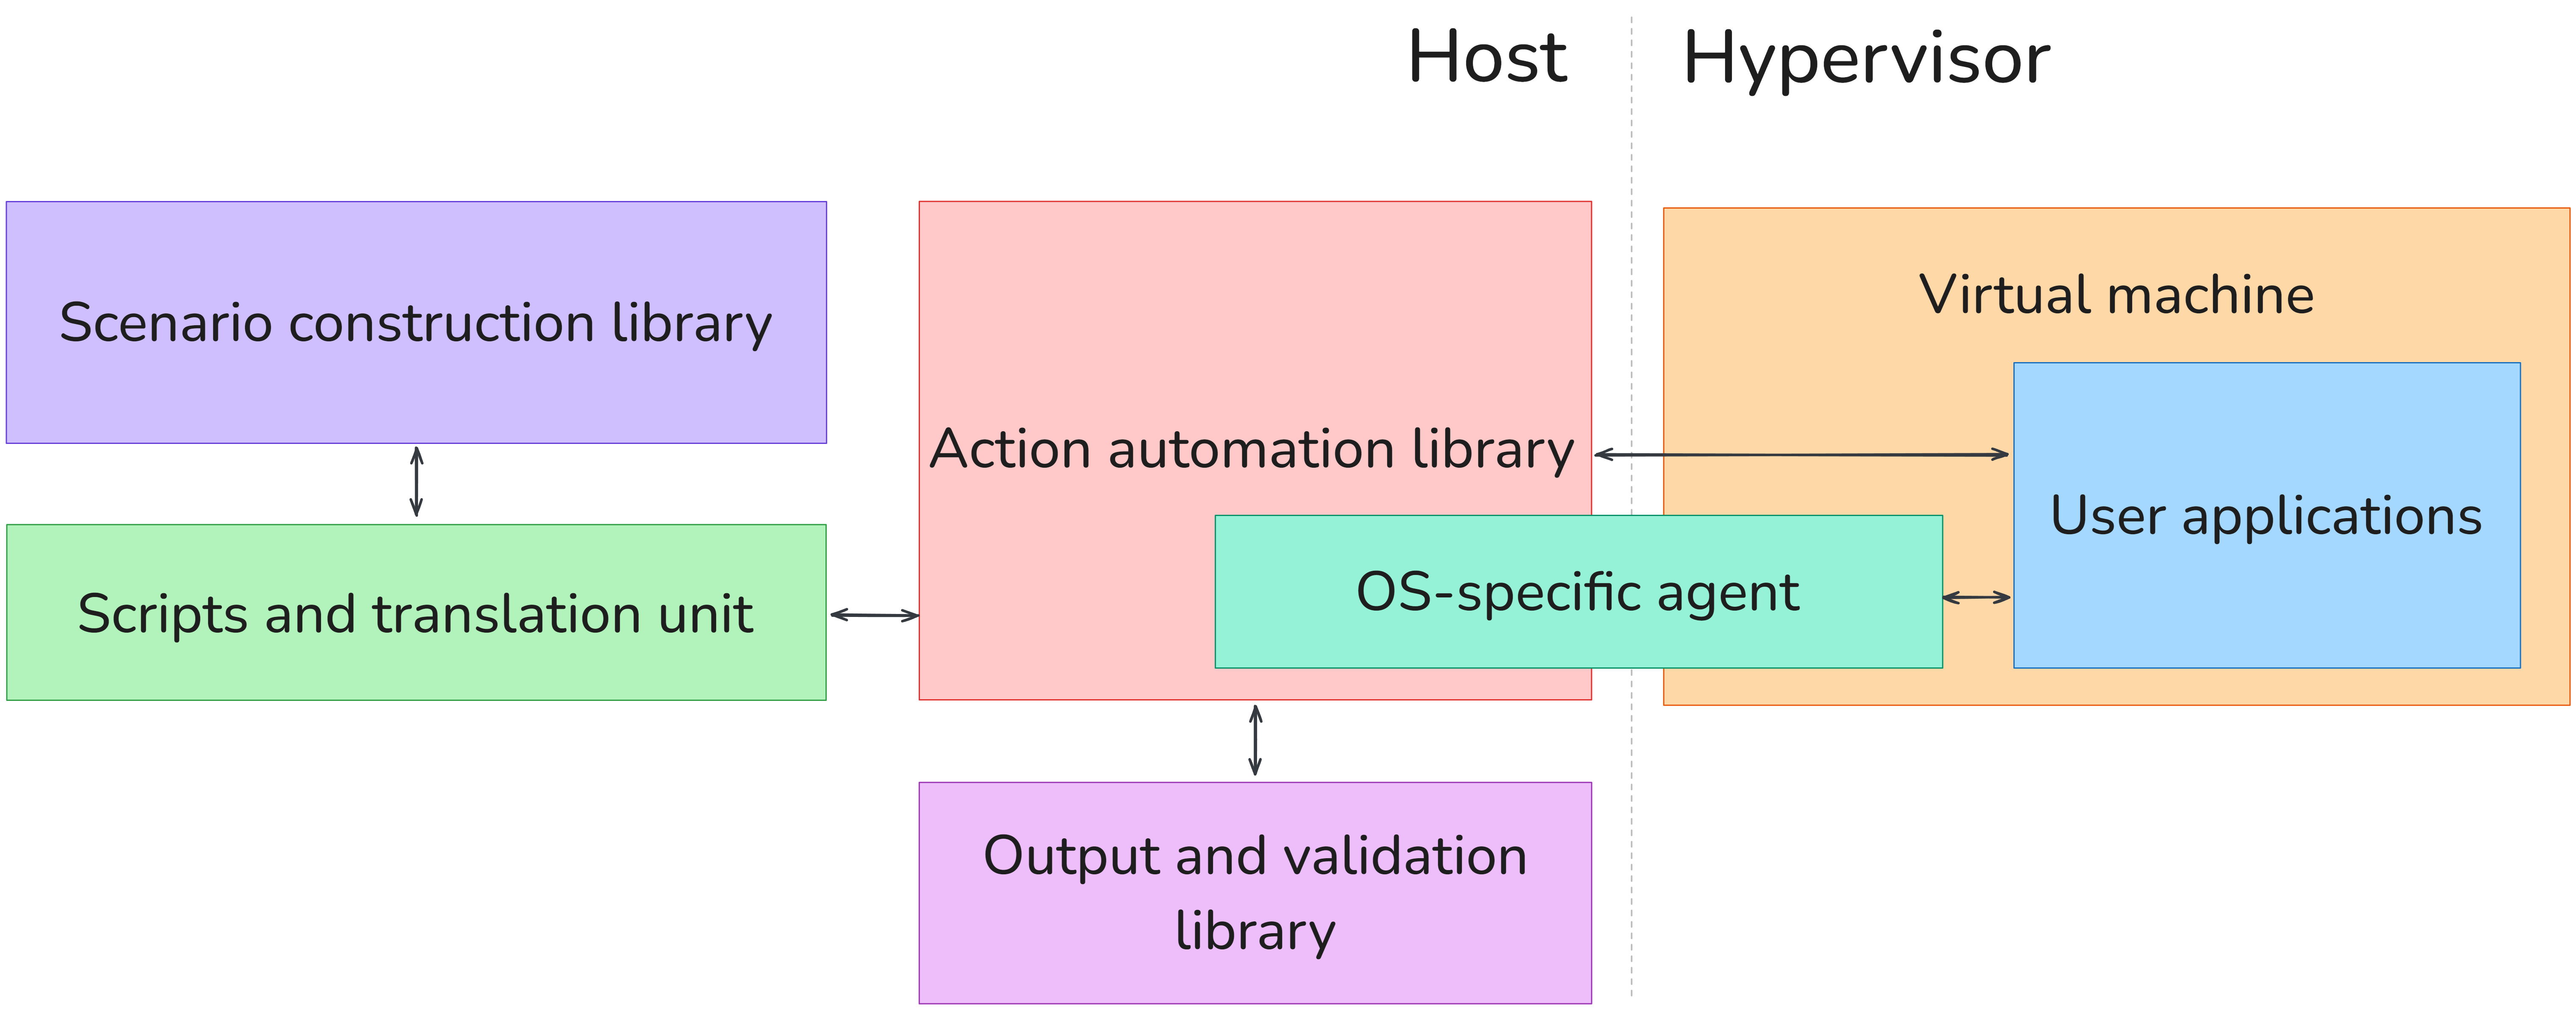
\includegraphics[width=1\linewidth]{architecture-simple.png}
\caption{Simplified AKF architecture
diagram}\label{fig:architecture-simple}
\end{figure}

AKF's seven top-level modules can be grouped into three distinct
concepts, each covering a specific chapter.

The first set of modules is responsible for artifact generation. This
encompasses three major systems - a hypervisor and its associated SDK,
an OS-specific agent, and \passthrough{\lstinline!akflib!}.
\passthrough{\lstinline!akflib!} is a Python library containing the
abstract interfaces and concrete implementations necessary to generate
artifacts and datasets. This includes routines for directly interacting
with hypervisors, issuing commands to virtual machines, and directly
modifying disk images. This library is also the foundation for
OS-specific agents, which carry out actions on the virtual machine on
behalf of the host. These modules are described in greater detail in
\autoref{chapter-four} and correspond to the \emph{action
automation library}, the \emph{OS-specific agent}, and the \emph{virtual
machine} (as well as the \emph{user applications} running on the
machine).

The second set of modules is responsible for logging and reporting. This
encompasses independent libraries for generating outputs and ground
truth, as well as the various logging-related mechanisms contained
throughout the artifact generation libraries. These modules are
responsible for exporting and documenting artifacts generated by AKF; in
particular, they make heavy use of CASE, a standardized ontology for
documenting the contents of forensic datasets
\cite{caseyAdvancingCoordinatedCyberinvestigations2017}. This is
covered in \autoref{chapter-five} and corresponds to the
\emph{output and validation library} and any associated components
within the \emph{action automation library}.

The final set of modules is responsible for invoking AKF itself and
supporting scenario development. AKF is an \emph{imperative}
synthesizer, which means that commands are written and executed using an
imperative language (Python 3) that dictates precisely \emph{how}
artifacts should be created. However, AKF also supports a
\emph{declarative} syntax, which allows users to specify \emph{what}
forensic artifacts should be generated without the need to understand
the AKF libraries and write actual Python code. These are discussed in
\autoref{chapter-six} and covers the \emph{scenario
construction library}, the \emph{translation unit}, and any scripts that
leverage AKF libraries. We also discuss the use of generative AI tools
for constructing individual artifacts and declarative scenarios.

The following three chapters will focus on these module groups. In
simpler terms, this thesis addresses the following questions in order:

\begin{itemize}
\tightlist
\item
  How do we automate or streamline the generation of artifacts?
\item
  How do we document and report on the artifacts and datasets that are
  generated?
\item
  Given the solutions that address these two questions, how do we
  actually use them to build scenarios?
\end{itemize}

\chapter{Action automation}\label{chapter-four}

At the core of every synthesizer is the ability to generate forensic
artifacts as part of a larger scenario; this chapter addresses the AKF
modules responsible for automating artifact generation, depicted in
\autoref{fig:actions-simple} below. The detailed diagrams for these
modules are part of \autoref{appendix-a}, depicted in
\autoref{fig:architecture-full-b} and \autoref{fig:architecture-full-d}.

\begin{figure}[h]
\centering
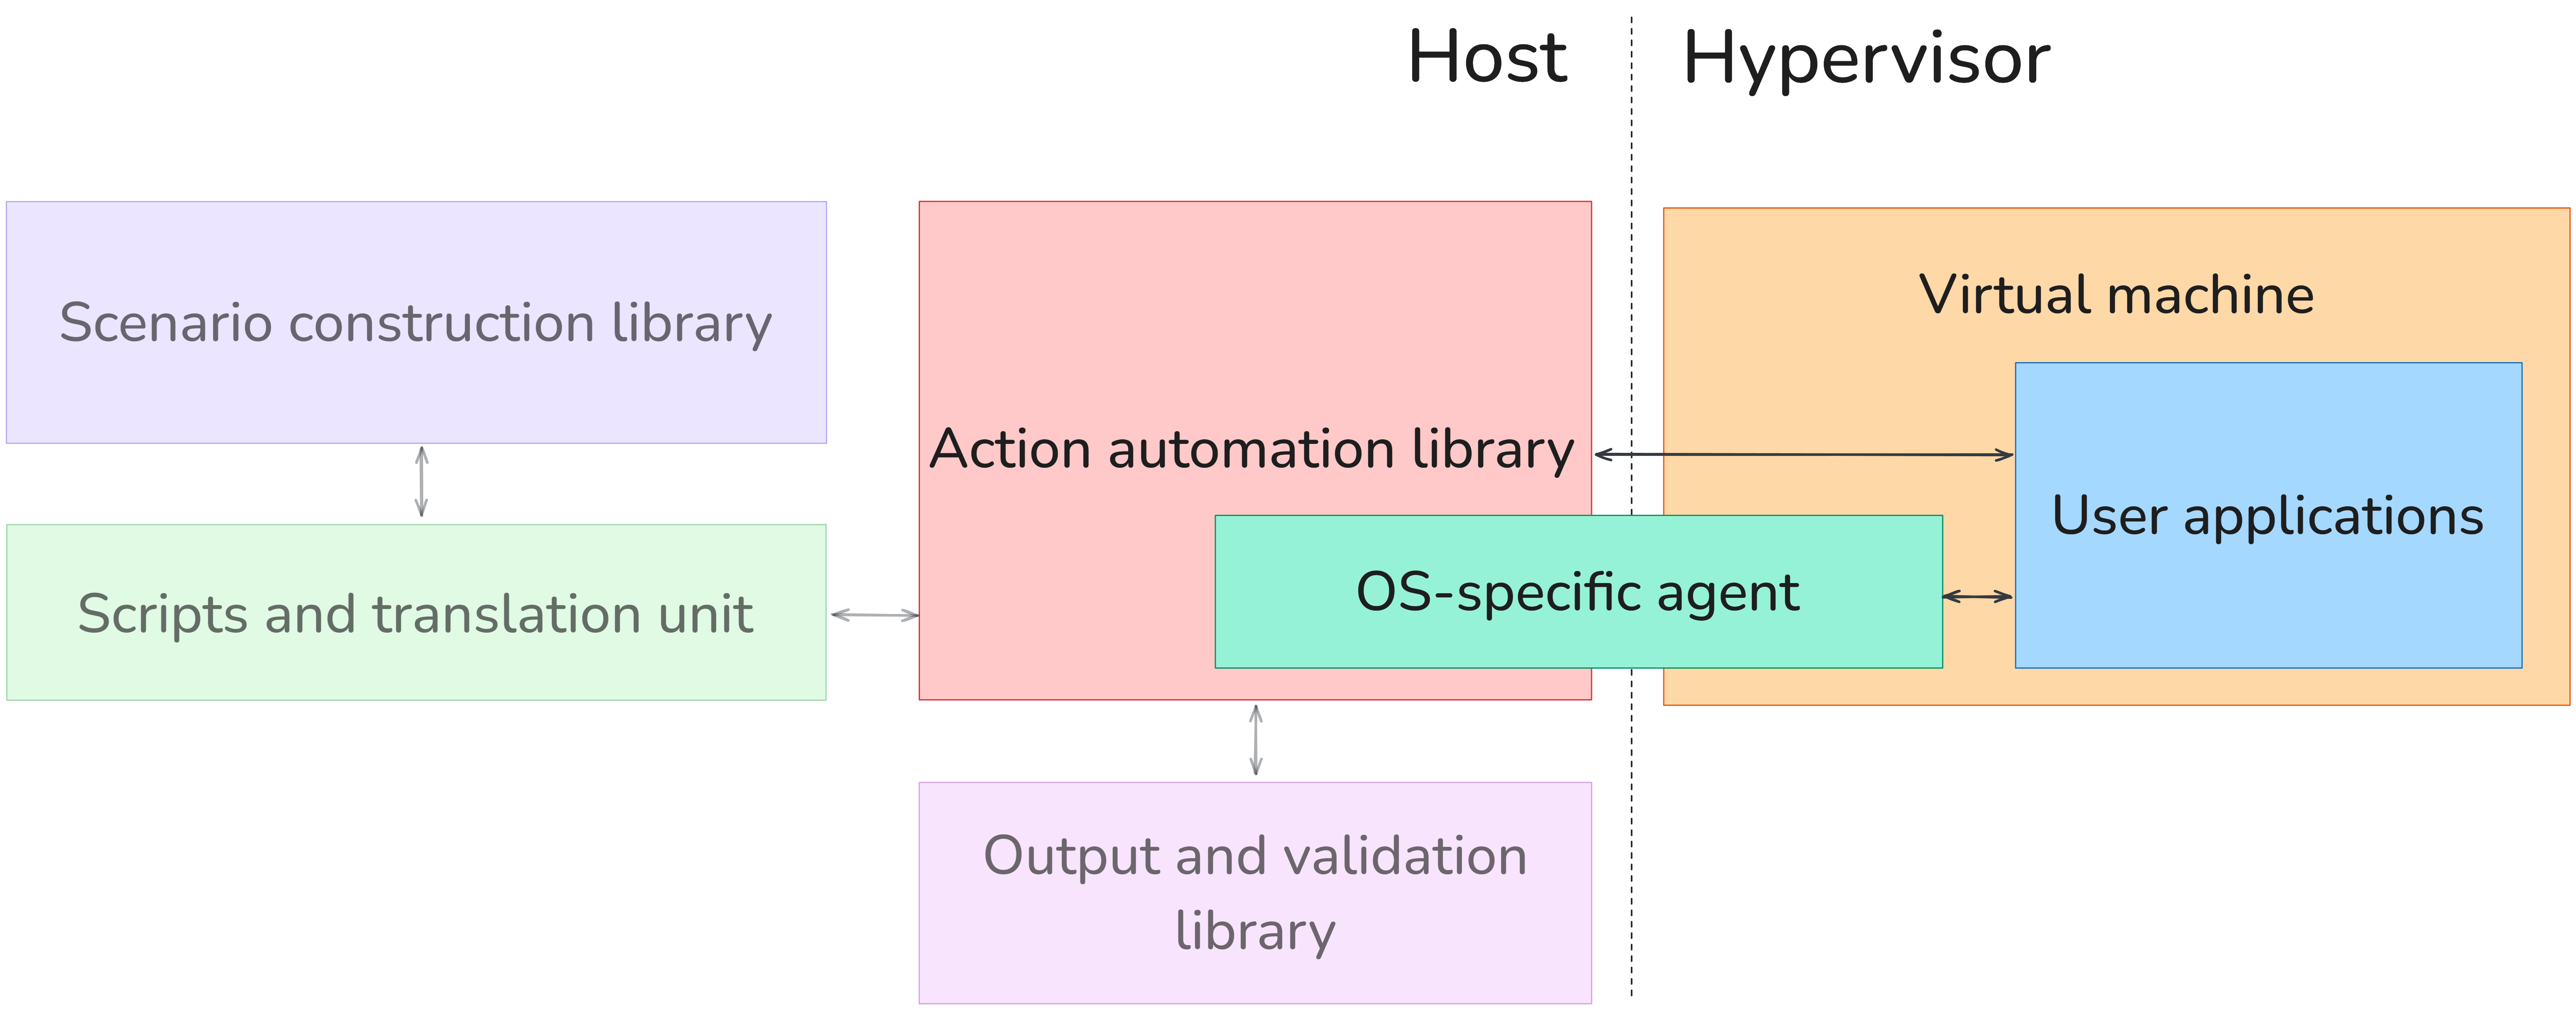
\includegraphics[width=1\linewidth]{actions-simple.png}
\caption{Simplified AKF architecture diagram for scenario construction
modules}\label{fig:actions-simple}
\end{figure}

Each of the synthesizers described in \autoref{analysis-of-existing-synthesizers} takes one of three
approaches to artifact generation, as partly described by Scanlon et al.
\cite{scanlonEviPlantEfficientDigital2017}:

\begin{itemize}
\tightlist
\item
  \textbf{Physical}: No virtualization of software or hardware ever
  occurs; data is written directly to the target medium, such as a disk
  image or virtual hard drive.
\item
  \textbf{Agentless logical}: The synthesizer interacts with a live VM
  to generate artifacts. Interaction is achieved without the need for
  custom software to be installed on the VM; instead, actions are
  achieved using the hypervisor itself or a remote management tool
  native to the virtualized operating system.
\item
  \textbf{Agent-based logical}: The synthesizer interacts with a
  dedicated client, or agent, on a live VM to carry out actions. The VM
  must have the agent installed before any interaction can occur.
\end{itemize}

These three approaches are not mutually exclusive within a single
synthesizer, though many prior synthesizers have used only one approach
to generate artifacts. \autoref{tbl:prior-techniques} below denotes the
approaches used by each of the synthesizers previously discussed. Where
source code is unavailable, a best effort was made to identify the
approach used by a particular synthesizer based on its published paper,
if one exists; otherwise, the entire row contains question marks.


{
\small % 10pt font
\setstretch{1} % Single spacing
\begin{longtable}[]{@{}
  >{\raggedright\arraybackslash}p{(\linewidth - 6\tabcolsep) * \real{0.2}}
  >{\raggedright\arraybackslash}p{(\linewidth - 6\tabcolsep) * \real{0.2666}}
  >{\raggedright\arraybackslash}p{(\linewidth - 6\tabcolsep) * \real{0.2666}}
  >{\raggedright\arraybackslash}p{(\linewidth - 6\tabcolsep) * \real{0.2666}}
@{}}
\caption{Summary of artifact generation techniques in prior synthesizers}\label{tbl:prior-techniques} \\
\toprule\noalign{}
\begin{minipage}[b]{\linewidth}\raggedright
Synthesizer
\end{minipage} & \begin{minipage}[b]{\linewidth}\raggedright
Physical
\end{minipage} & \begin{minipage}[b]{\linewidth}\raggedright
Agentless
\end{minipage} & \begin{minipage}[b]{\linewidth}\raggedright
Agent-based
\end{minipage} \\
\midrule\noalign{}
\endhead
\bottomrule\noalign{}
\endlastfoot
\textbf{FALCON} \cite{adelsteinAutomaticallyCreatingRealistic2005},
2005 & ? & ? & ? \\
\textbf{CYDEST} \cite{bruecknerAutomatedComputerForensics2008}, 2008
& ? & ? & ? \\
\textbf{Forensig2}
\cite{mochForensicImageGenerator2009,mochEvaluatingForensicImage2012},
2009 & Yes (filesystem mounting; filesystem-independent editing) & Yes
(over SSH only) & No \\
\textbf{D-FET} \cite{williamCloudbasedDigitalForensics2011}, 2011 &
Yes (filesystem mounting; filesystem-independent editing) & No & No \\
\textbf{SFX} \cite{russellForensicImageDescription2012}, 2012 & Yes
(filesystem mounting) & No & No \\
\textbf{Yannikos et al.} \cite{yannikosDataCorporaDigital2014}, 2014
& ? & ? & ? \\
\textbf{ForGeOSI} \cite{maxfraggMaxfraggForGeOSI2023}, 2014 & No &
Yes (hypervisor interfaces) & No \\
\textbf{ForGe} \cite{vistiAutomaticCreationComputer2015}, 2015 & Yes
(filesystem-aware editing) & No & No \\
\textbf{ForGen} \cite{jjk422Jjk422ForGen2019}, 2016 & No & No &
No \\
\textbf{EviPlant} \cite{scanlonEviPlantEfficientDigital2017}, 2017 &
Yes (filesystem-independent editing) & No & Yes (unknown mechanism) \\
\textbf{VMPOP} \cite{parkTREDEVMPOPCultivating2018}, 2018 & No & Yes
(hypervisor interfaces) & No \\
\textbf{hystck} \cite{gobelNovelApproachGenerating2020}, 2020 & No &
No & Yes (Python agent) \\
\textbf{TraceGen} \cite{duTraceGenUserActivity2021}, 2021 & No & No
& Yes (unknown mechanism) \\
\textbf{ForTrace} \cite{gobelForTraceHolisticForensic2022}, 2022 &
No & No & Yes (Python agent) \\
\end{longtable}
}


There are advantages and disadvantages to each approach, in addition to
requiring distinct implementation techniques for each. The remainder of
this chapter analyzes each of these three approaches in greater detail,
describing the implementation details of prior synthesizers and
comparing them to those of AKF's.

More specifically, this chapter addresses the functionality of the
action automation library (\passthrough{\lstinline!akflib!}) to generate
artifacts by either interacting with a live virtual machine or by
directly editing disk images stored on the host. We explore how logical
artifacts are generated at a lower level using hypervisor APIs and an
OS-specific agent running on the virtual machine. We conclude by
describing the generation of physical artifacts through direct
filesystem and disk image editing.

\section{Agentless artifact
generation}\label{agentless-artifact-generation}

\textbf{Agentless artifact creation} describes one of two general
techniques. The first is emulating ``normal'' human interaction by
leveraging virtualized human interfaces -- such as the monitor,
keyboard, and mouse -- to directly manipulate a GUI-based operating
system. The second is using (remote) management utilities included with
the operating system, typically an interactive shell.

AKF allows users to perform agentless artifact creation through a
hypervisor-agnostic interface; a concrete implementation of this
interface using VirtualBox is provided. This VirtualBox-specific
functionality is derived mainly from ForGeOSI
\cite{maxfraggMaxfraggForGeOSI2023}, which uses the VirtualBox SDK
and a Python implementation of the VirtualBox COM API
\cite{larsonSethmlarsonVirtualboxpython2025} to carry out the vast
majority of its tasks. This was adapted in VMPOP
\cite{parkTREDEVMPOPCultivating2018}, which also introduced the
notion of a generic hypervisor interface that allows for synthesizer
routines to use arbitrary hypervisors so long as required functionality
is implemented.

Note that the use of hypervisor-specific guest software, such as
VirtualBox Guest Additions and VMWare Tools, is treated as an agentless
approach for this thesis. Although this inherently requires installing
``unusual'' software on the virtual machine, it is very distinct from
typical user software. In many cases, artifacts generated by hypervisor
guest software can be identified, isolated, and ignored.

Relevant AKF submodules for agentless generation are depicted as opaque
elements in \autoref{fig:action-agentless}.

\begin{figure}[h]
\centering
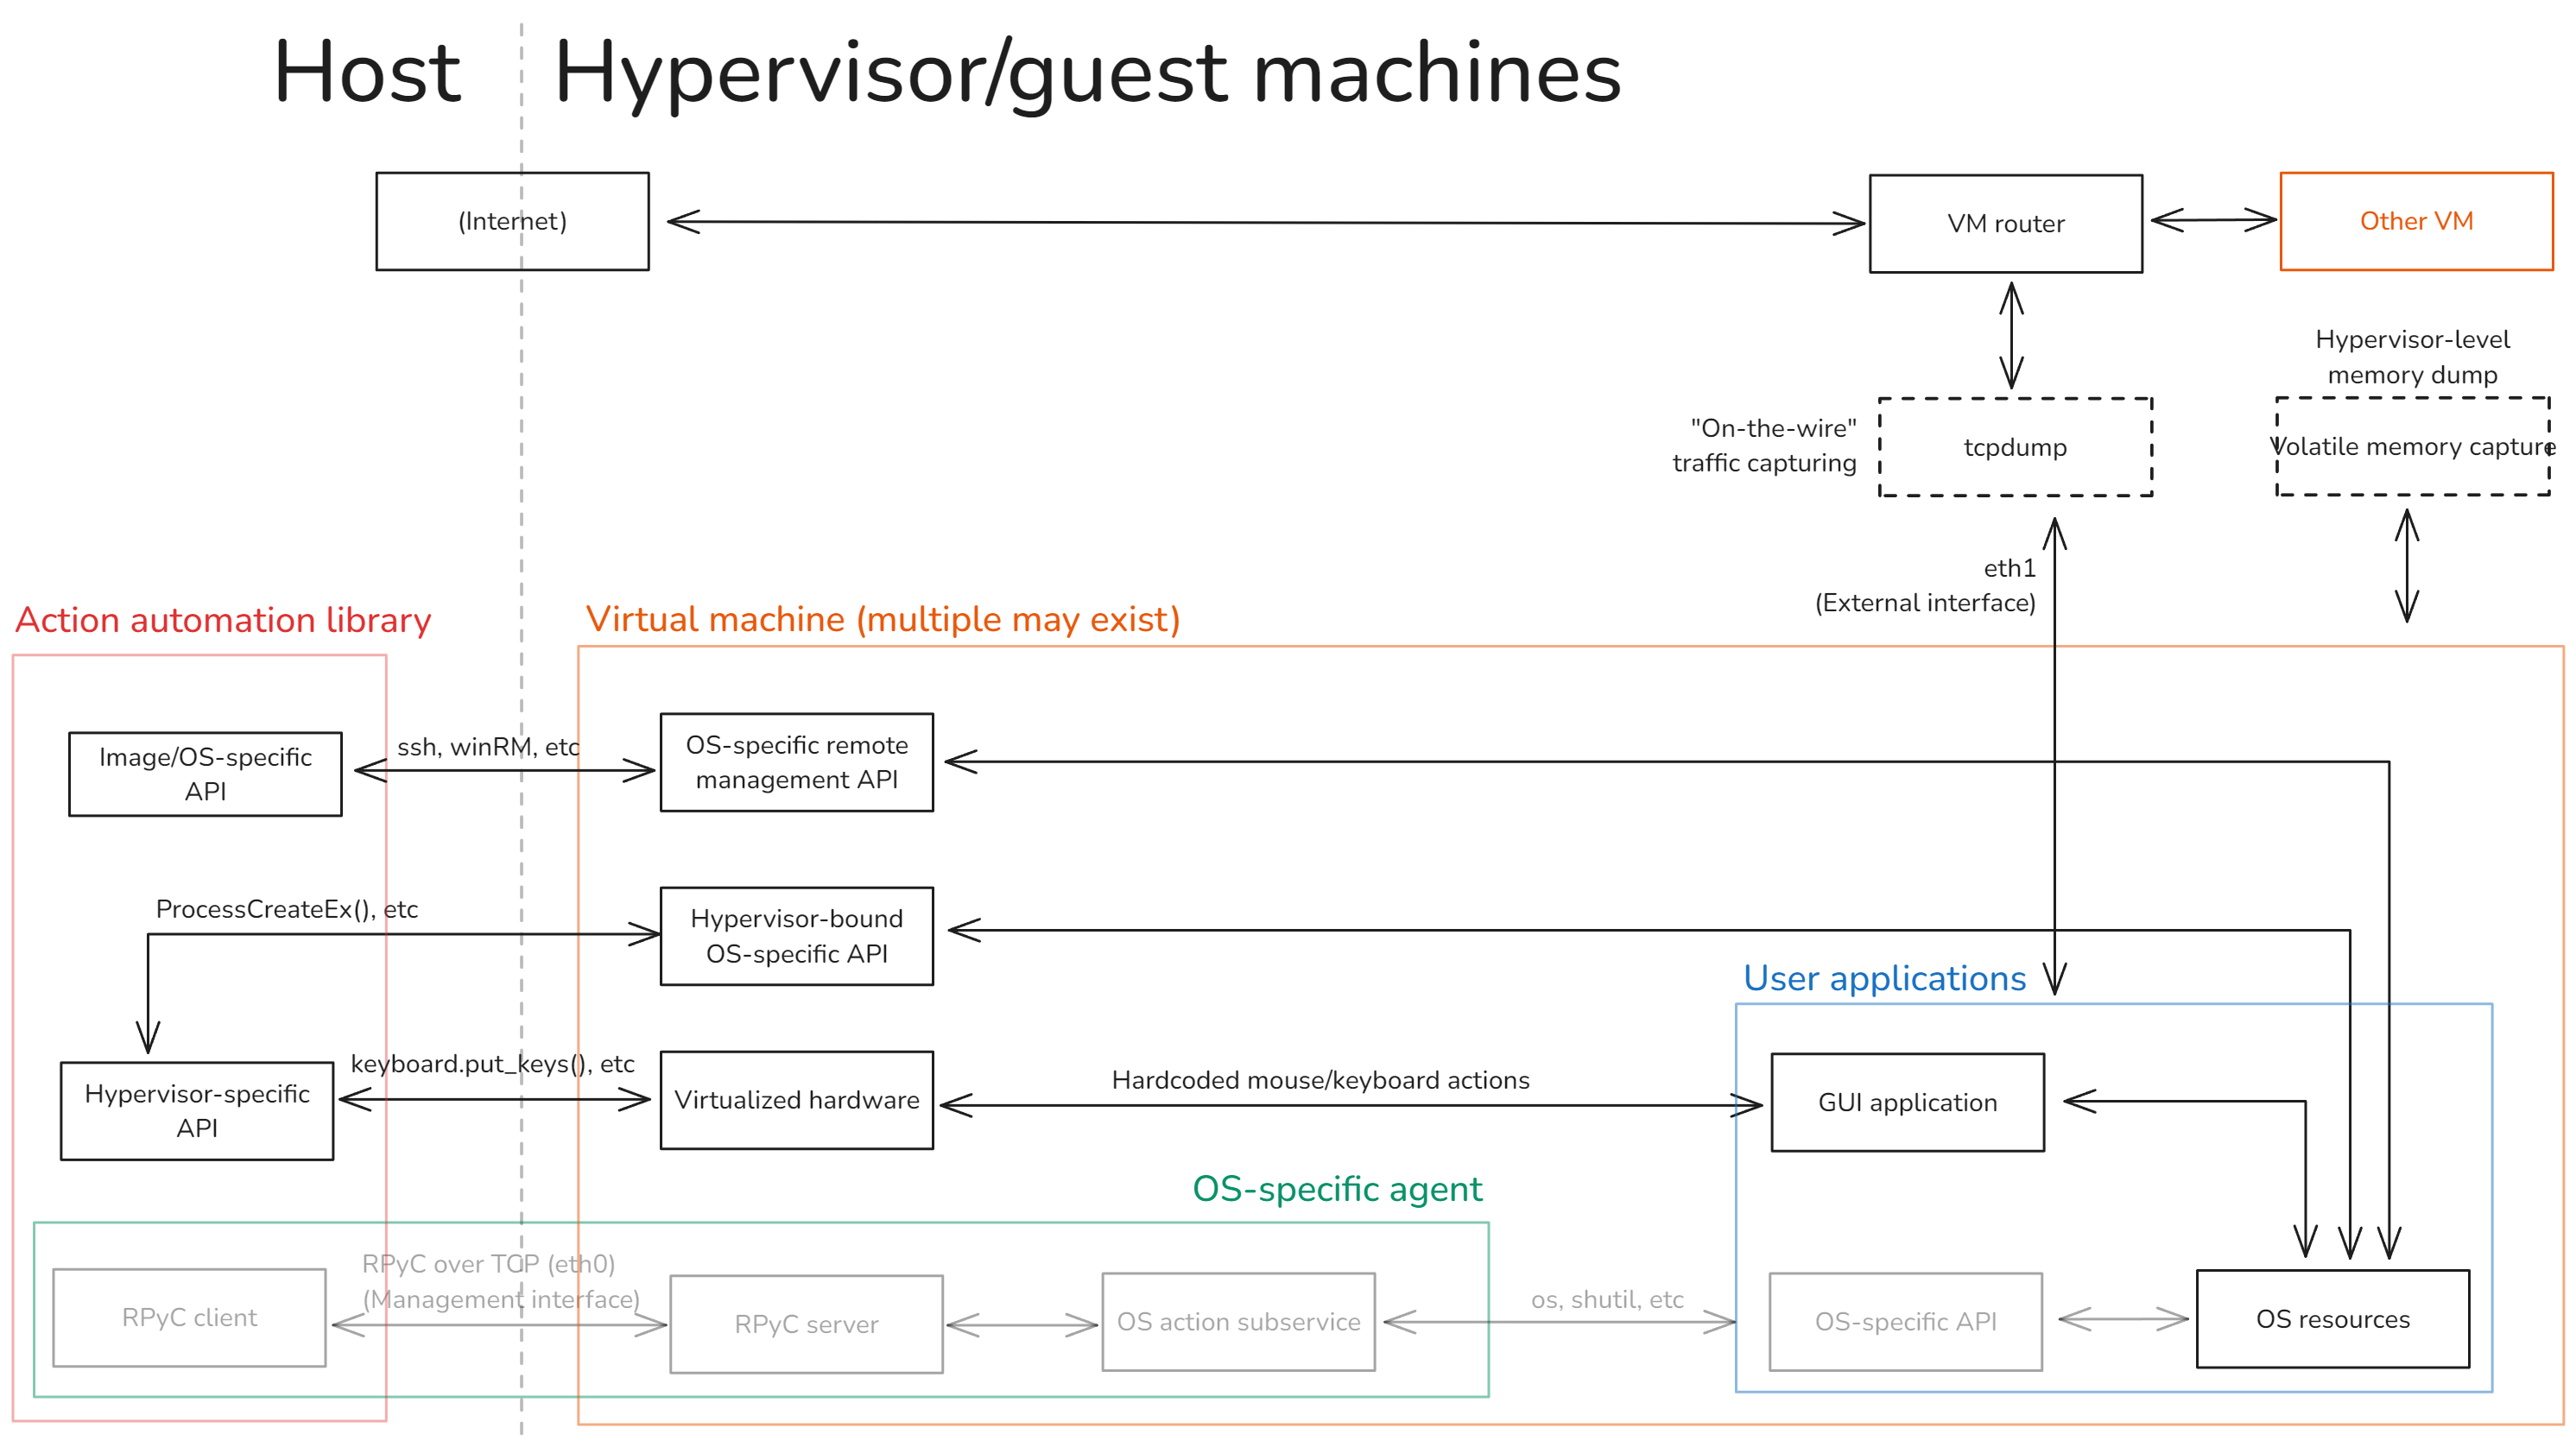
\includegraphics[width=1\linewidth]{action-agentless.png}
\caption{Abridged submodule diagram for agentless artifact
creation}\label{fig:action-agentless}
\end{figure}

\subsection{Human interfaces}\label{human-interfaces}

The use of human input devices -- the keyboard and mouse -- is the
primary approach taken by VMPOP \cite{parkTREDEVMPOPCultivating2018}
and ForGeOSI \cite{maxfraggMaxfraggForGeOSI2023} to generate
artifacts. For example, VMPOP uses a sequence of keyboard strokes to
focus and interact with UI elements, such as clearing User Account
Control dialogs on Windows or starting applications with Win+R. It
achieves this by making calls to the VirtualBox API, which issues
scancodes to the virtual machine.

This approach most accurately reflects how an actual human would
interact with a machine. As a result, this greatly reduces the
irrelevant data generated as a result of synthesizer operation. However,
this often leads to verbose scripts that are only capable of performing
very specific actions. The keyboard and mouse actions required to
fulfill a particular action can change significantly between versions of
the same application, versions of the same operating system, and varying
screen sizes. For example, VMPOP handles User Account Control (UAC)
prompts on machines prior to Windows 7 by sending an Alt+Tab keystroke
to the machine, clicking the mouse at the center of the screen to focus
the UAC prompt, and then sending Alt+C to accept the prompt. On machines
running Windows 7 or later, this is instead achieved by focusing the UAC
prompt with the mouse and then sending Alt+Y to accept the prompt.

Similarly, VMPOP interacts with browsers exclusively through the use of
keyboard shortcuts. VMPOP supports simple interactions with a small
number of websites, such as logging into Microsoft or Google accounts,
but is dependent on the form elements remaining the same over time. That
is, VMPOP does not inspect the contents of the current webpage to
perform actions; it cannot react to design changes. If the page has new
focusable elements, the same keystroke sequence may no longer achieve
the desired effects. This lack of runtime logic, which amounts to
operating a computer with the monitor off, leads to brittle scripts that
can be tedious to fix and update.

AKF's generic hypervisor interface provides functions for both mouse and
keyboard actions. While this is theoretically sufficient to emulate
nearly all actions that a human would normally perform with a mouse and
keyboard, the AKF agent (as described in \autoref{the-akf-agent}) also exposes a more flexible mouse
and keyboard automation API that is strongly preferred over the
VirtualBox interface. More generally, the AKF agent leverages automation
frameworks capable of runtime UI analysis, reducing the inflexibility of
application-specific scripts.

TraceGen \cite{duTraceGenUserActivity2021} notes that the ideal
future is to use computer vision and AI to automate user actions from
high-level prompts. Performing a Google search in a specific browser
would currently require a sequence of predefined keystrokes, assuming an
agentless approach is needed. Future advancements in LLMs may make it
possible to allow a machine to perform arbitrarily complex tasks on a
GUI-based operating system using natural language -- an approach that
can be integrated into AKF in the future, as addressed in \autoref{open-ended-automation-with-ai}.

\subsection{Management utilities}\label{management-utilities}

The alternative is to use existing management utilities which are native
to the virtualized operating system and are capable of carrying out
commands. This approach can also be divided into two categories: local
management utilities, such as Bash and PowerShell, and remote management
utilities, such as SSH servers and WinRM.

Local management utilities typically refer to scripting languages that
are available as part of the operating system and can be used to manage
most or all operating system resources. For example, PowerShell allows
users to modify registry keys, invoke applications, create users, and
more. Similarly, any standard Linux shell, such as Bash or Zsh, can be
used to install packages and run various command-line applications.
These shells can be invoked by either opening and focusing a terminal
window (for example, through the Win+R shortcut on Windows) or directly
executing scripts through hypervisor guest additions.

In particular, VMPOP \cite{parkTREDEVMPOPCultivating2018} makes
heavy use of local management utilities; it implements much of its
functionality through a collection of PowerShell and batch scripts. For
example, VMPOP allows users to focus a window by process ID, process
name, or window title. This is achieved by getting a PowerShell handle
to the process using \passthrough{\lstinline!Get-Process!}, using
\passthrough{\lstinline!Add-Type!} to add a local C\# function that is
capable of sending keyboard events through
\passthrough{\lstinline!user32.dll!}, and then holding the Alt key while
using \passthrough{\lstinline!AppActivate!} to focus the window and
bring it to the foreground. VMPOP leverages similar scripts for
launching and terminating processes by name, uninstalling programs,
creating a Windows restore point, and more.

Similarly, remote management utilities allow a remote device to invoke
local management utilities, typically over an SSH server or WinRM. In
most synthesizer architectures, remote management utilities require that
the host and guest machines can communicate with each other. This is
typically achieved through a NAT or host-only interface managed by the
hypervisor. This approach is taken by Forensig2
\cite{mochForensicImageGenerator2009}, which exclusively connects to
a running SSH server on a virtual machine to carry out user actions.

The use of remote management utilities to automate actions typically
undertaken by users is not uncommon, especially with the prevalence of
infrastructure as code solutions. For example, the open-source Ansible
framework simplifies the configuration of Windows and Linux devices to
simple, YAML-based files called ``playbooks.'' These playbooks contain a
sequence of tasks to perform, such as installing packages, managing
local user accounts, and running scripts, which are executed on multiple
remote machines in parallel. (Ansible's high-level scripting language is
the inspiration for AKF's declarative scripting language, described in
\autoref{declarative-usage}.)

It is worth noting that although this approach does not require
installing new software on the machine, most operating systems perform
some degree of logging when their management utilities are invoked. For
example, the \passthrough{\lstinline!sshd!} daemon logs connections
regardless of whether a NAT or host-only network interface is used. This
behavior may make it difficult to separate or remove logs unrelated to a
scenario. Similarly, the invocation of PowerShell scripts generates
event logs, which can be particularly noisy if Script Block Logging
(which logs the execution and content of all PowerShell scripts) is
enabled.

AKF inherits the capabilities of VMPOP, allowing users to leverage the
VirtualBox API and Guest Additions for various actions. For example,
users can mount shared directories and copy artifacts from the host to
the guest machine. However, AKF does not currently implement any
agentless OS- or application-specific functionality through this method;
many of the actions and artifacts previously generated through
OS-specific scripts in VMPOP \cite{parkTREDEVMPOPCultivating2018}
and other synthesizers can be implemented with greater flexibility
through the agent. How this flexibility is achieved, as well as why it
is the preferred method for implementing application-specific
functionality, is described in the following section.

\section{Agent-based artifact
generation}\label{agent-based-artifact-generation}

\textbf{Agent-based artifact creation} involves the use of a dedicated
executable on the VM that serves as an interface between the host
machine and the guest machine. This program runs commands natively on
the virtual machine on behalf of the host machine, accepting commands
over a dedicated network interface. This allows for greater flexibility
and more complex actions to be taken when compared to agentless
approaches. In particular, it allows application-specific functionality
to be implemented using existing automation frameworks such as Selenium
\cite{SeleniumHQSelenium2025}, Playwright
\cite{MicrosoftPlaywrightpython2025}, and PyAutoGUI
\cite{sweigartAsweigartPyautogui2025}.

It is worth noting that agent-based artifact creation often leads to the
generation of extraneous artifacts that would never be seen in a
real-world dataset. For example, agents often do not interact with
applications in the same way that a human would, possibly creating
additional artifacts that would not exist if a human had performed the
same actions. As a result, the synthesizer should document
synthesizer-related artifacts that can be ignored for educational and
testing purposes.

Relevant AKF submodules for agent-based generation are depicted as
opaque elements in \autoref{fig:action-agent}.

\begin{figure}[h]
\centering
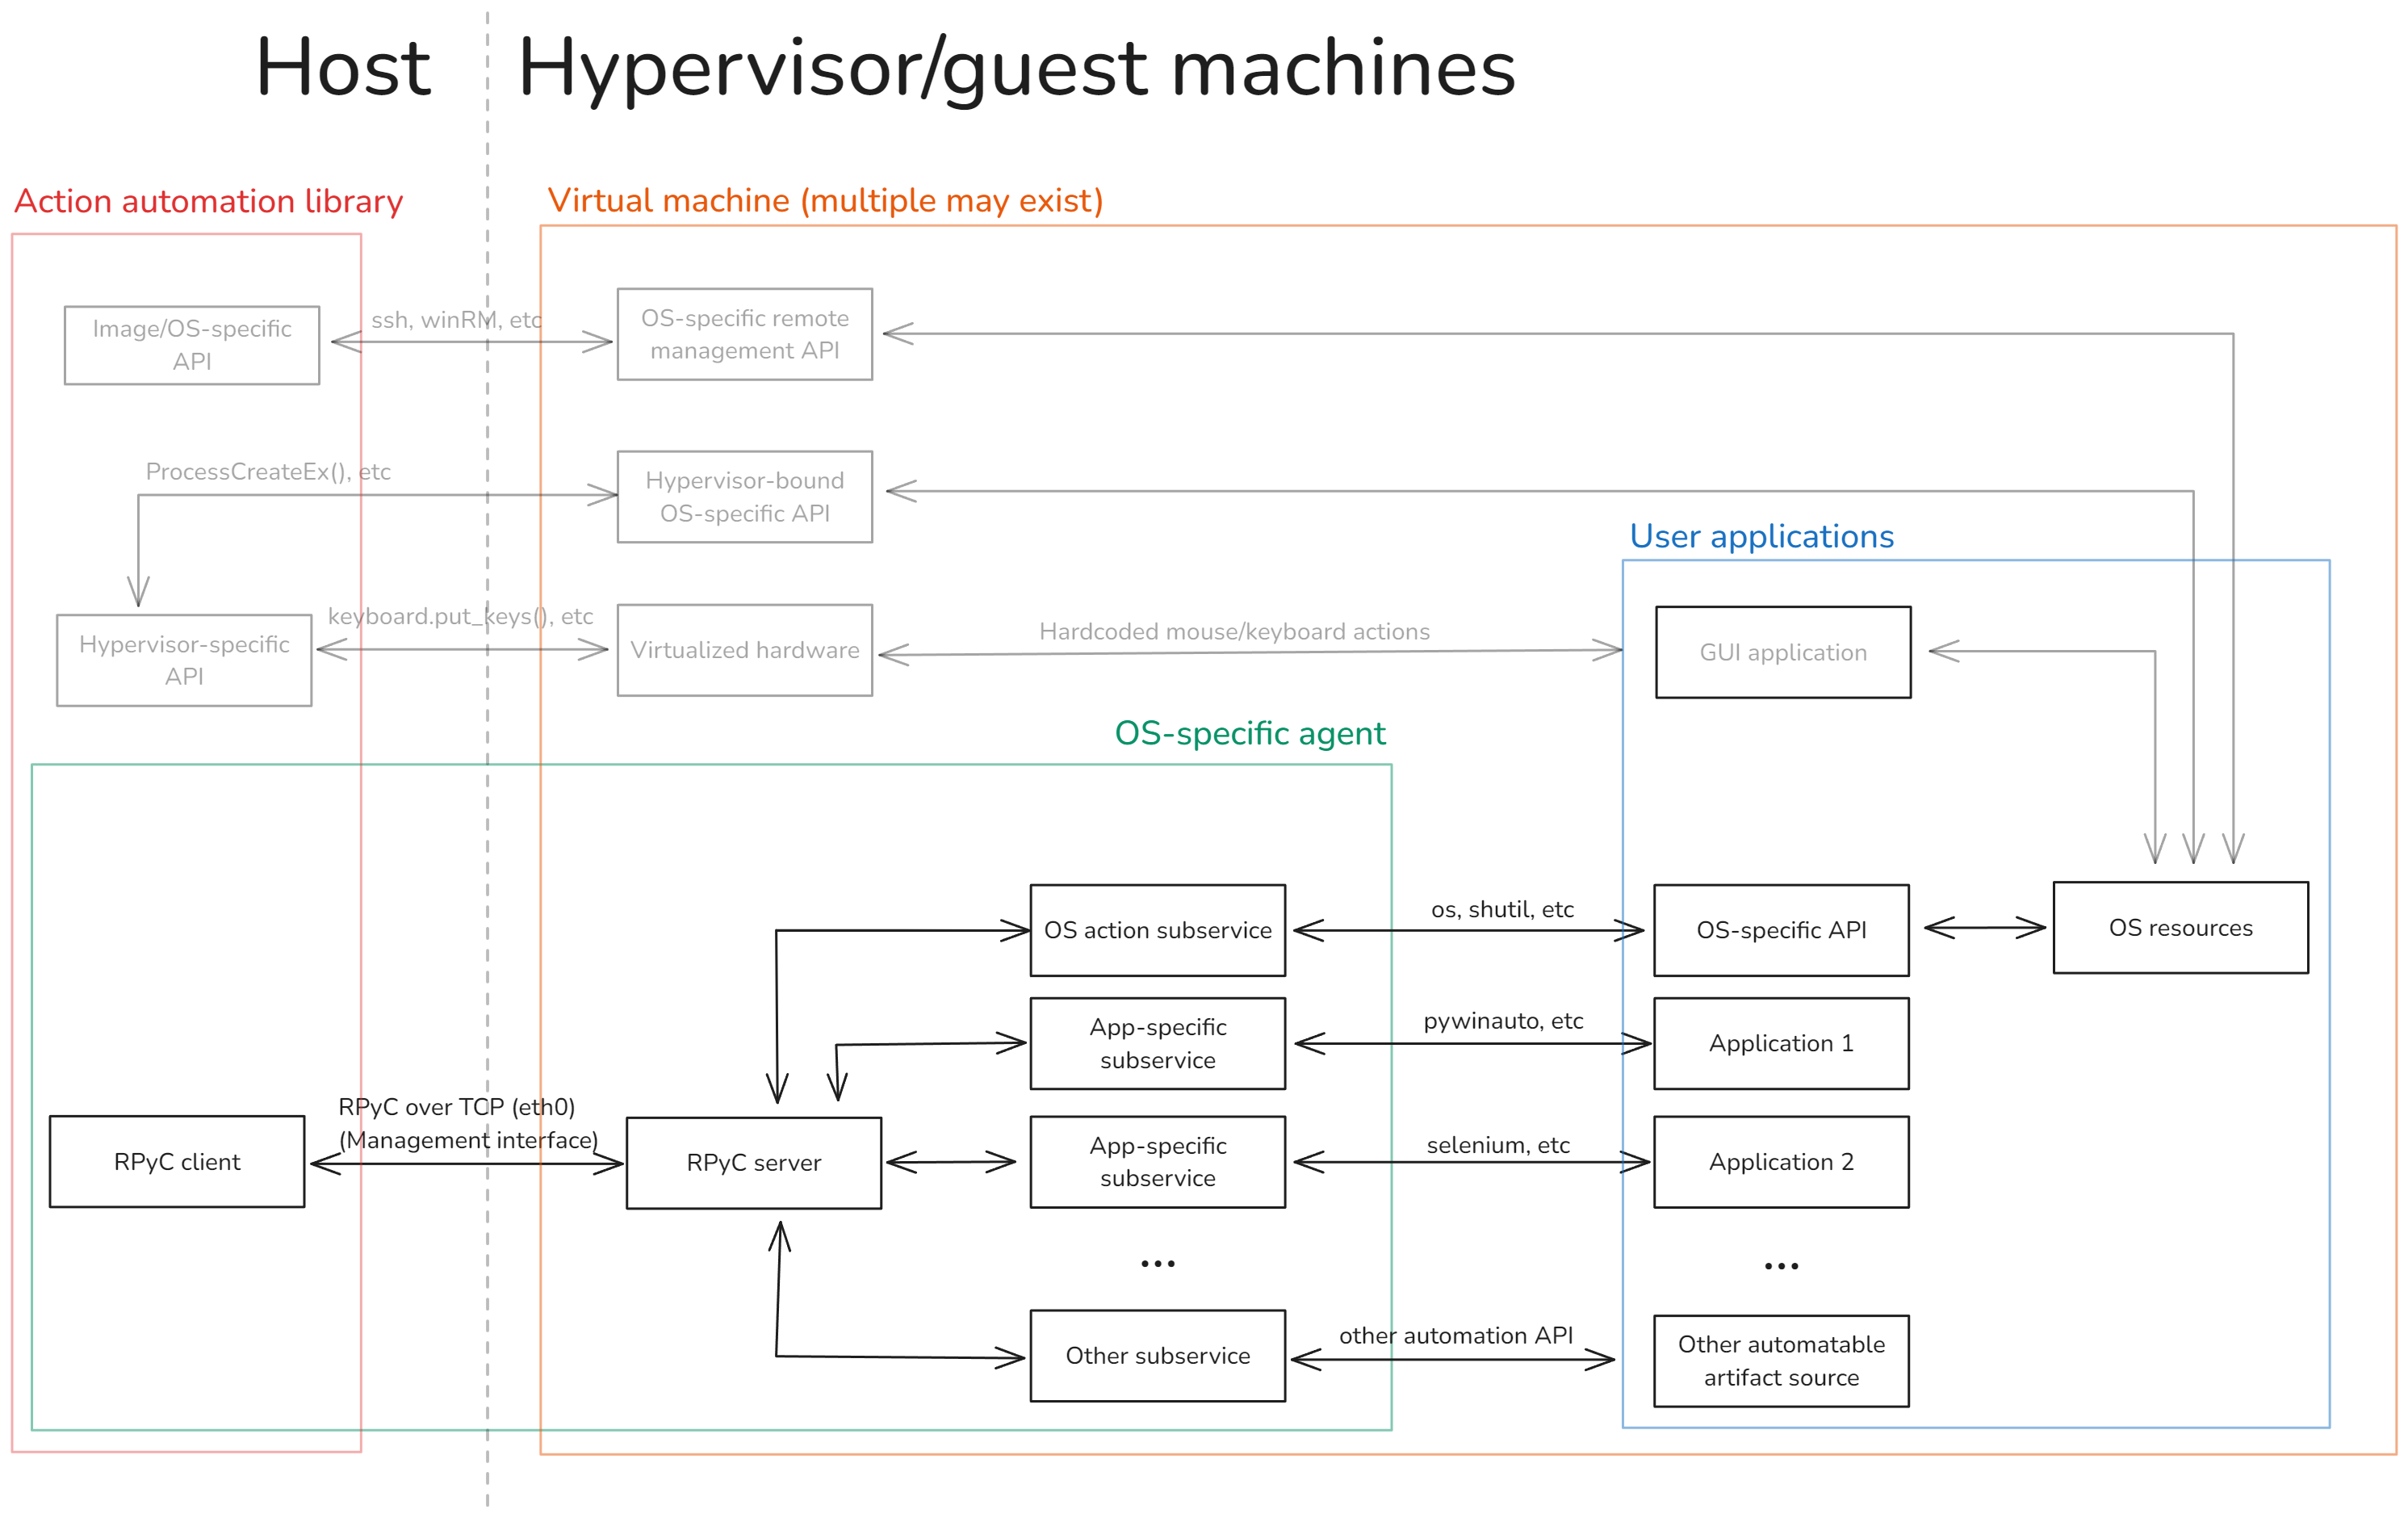
\includegraphics[width=1\linewidth]{action-agent.png}
\caption{Abridged submodule diagram for agent-based artifact
creation}\label{fig:action-agent}
\end{figure}

\subsection{Analysis of the ForTrace
agent}\label{analysis-of-the-fortrace-agent}

Agent-based artifact creation is the approach taken by hystck/ForTrace
\cite{gobelNovelApproachGenerating2020,gobelForTraceHolisticForensic2022},
which refers to its agent as an ``interaction manager.'' Because
ForTrace provides extensive agent functionality and is by far the most
mature synthesizer, AKF's agents borrow heavily from ForTrace's
approach. We briefly describe ForTrace's implementation of agents here,
with a more detailed analysis in \autoref{comparison-of-fortrace-and-akf-agents}.

ForTrace agents are simply an entire copy of the ForTrace codebase
copied over to the virtual machine -- that is, the ``agent'' and
``server'' share the same codebase but have different entry points and
use different parts of the ForTrace library. Communication between the
agent and the server occurs over a dedicated TCP socket using a simple
ASCII-based protocol; to execute commands, the server sends a
space-delimited string containing the application, function, and
arguments to run. Results are similarly returned by the agent as
structured ASCII messages. These messages are typically sent over a
dedicated ``management'' network interface to exclude them from network
captures for scenario-related activities.

Application-specific functionality for agents is organized into
individual files (Python modules), where each file includes a set of
commands or actions for a single application. These files contain both
server-side code (the logic for \emph{constructing} the ASCII message)
and agent-side code (the logic for \emph{interpreting} the message and
\emph{executing} the command) as a set of classes with a common prefix.
This common prefix is used to automatically discover the corresponding
agent-side code given a command issued by the server-side code.

Two key implementation details should be noted here. First, commands are
sent through a simple string-based protocol. This simplicity makes it
easy to debug issues arising from the protocol itself, but is relatively
inflexible as a result. In particular, it is challenging to send complex
Python objects as arguments or return values since these objects often
cannot be easily serialized to a string without loss of information. An
example relevant to AKF is passing Playwright browser objects, which
contain an internal state that is difficult to extract and reconstruct
using strings alone.

The second implementation detail involves the discovery and execution of
commands indicated by the protocol. ForTrace depends on Python's runtime
introspection to discover the correct modules and functions to call
based on the contents of a command string, importing these modules
during runtime. While this is a valid approach, it is more complex (and
difficult to follow) than the approach taken by AKF.

\subsection{The AKF agent}\label{the-akf-agent}

AKF borrows heavily from the Python agent-based approach of ForTrace but
improves upon its architecture in several respects. Details of low-level
improvements over ForTrace's agent architecture are described in more
detail in \autoref{comparison-of-fortrace-and-akf-agents}.

Perhaps the most significant difference is the use of RPyC, a library
for symmetric remote procedure calls, for agent communication
\cite{TomerfilibaorgRpyc2025}. Although the RPyC protocol is
symmetric, it is often used in typical client-server architectures to
allow clients to manipulate remote Python objects as if they were local
objects, as well as invoke remote (server) functions using local
(client) parameters. Delegating the serialization and deserialization of
complex objects to RPyC allows us to perform complex operations that
would have been difficult to implement with the simple string-based
protocol of ForTrace.

In ``new-style'' RPyC, this is achieved by running a \emph{service} on
the device where remote operations should be performed. Services expose
a set of functions and attributes that may be accessed remotely by an
RPyC client, listening on a specified TCP port for requests to access
these exposed elements. Clients access these functions and attributes by
name as if they were local objects; arguments passed to functions are
serialized and deserialized in the background, as are the results of
function calls and attribute accesses.

AKF's application-specific functionality is divided into individual RPyC
``subservices'' created on demand. The agent's main loop is itself a
``root'' RPyC service that is responsible for creating and destroying
these subservices upon request; all subservices are known to the root
service at initialization, eliminating the need to perform runtime
introspection to find application-specific modules. These subservices
are analogous to the agent-side code of individual ForTrace modules,
interpreting arguments and executing commands on behalf of the host
machine.

Clients are largely decoupled from the server's implementation of
individual services; they do not directly call or import RPyC service
functions. Instead, they call these functions by name from an untyped
connection object. Because the exposed functions (as well as their
signatures) and attributes cannot be inferred from the raw RPyC
connection alone, clients can implement a typed, concrete API to
construct RPyC calls. This abstracts the raw RPyC call (and the
existence of an RPyC connection) away from the user while also providing
the signatures of remote functions where there would otherwise be none.
This allows for type checking and autocompletion during development.
This is analogous to the client-side code of individual ForTrace
modules, constructing messages to the agent to execute commands.

Additionally, because the RPyC service and the API to that service are
separable, this allows us to break the API (which is used in scenario
scripts) and the agent logic itself into two separate libraries. This
has two advantages -- it makes it significantly easier to build and
generate standalone executables using tools like PyInstaller
\cite{PyinstallerPyinstaller2025}, and it may also slightly reduce
the size of the agent when installed onto the virtual machine. Unlike
ForTrace, whose agent installation process requires a batch script
installing various libraries and Python through the Chocolatey package
manager, AKF's agent only requires that a single executable is copied
over and configured to run on startup (in addition to setting relevant
firewall rules). The agent setup process can be further simplified using
Vagrant, which is described in \autoref{setup-and-basic-usage}.

From an implementation and usability perspective, this design provides
three significant improvements over the ForTrace protocol. First, the
routing of functions is wholly delegated to RPyC. Instead of manually
constructing a message with the function name and its associated
parameters (as strings) over the network, the process of serializing
parameters and routing them to the correct function call is abstracted
away by RPyC.

Second, this allows us to pass and return arbitrarily complex objects
(for which we do not have to manually write the serialization and
deserialization logic). When passing complex objects from the agent to
the server or vice versa, a reference to the object is sent over the
network and wrapped by a \emph{proxy object}, which behaves like the
original object \cite{TheoryOperationRPyC}. Importantly, it is
usually not necessary to distinguish between local and remote/proxy
objects of the same type when writing code, which eliminates the extra
complexity of using proxies.

Finally, the ability to interact with complex remote objects allows us
to significantly reduce the actual code written as part of the API
exposed to the host. For example, there is no need to implement a
wrapper for every method available as part of a Playwright page object;
instead, a reference to the Playwright object \emph{running on the
virtual machine} can be given to the host machine. Instead of writing
individual methods for opening pages, navigating to specific elements,
and so on, we can simply use the methods that already exist in the
Playwright object -- any local calls on the host's proxy object will
lead to remote outcomes on the host, as desired. This, of course, does
not preclude the ability to write convenience methods for more complex
actions requiring the Playwright object.

The list of subservices supported by the AKF Windows agent is described
in \autoref{tbl:akf-applications} below. Although only three subservices
are implemented, each subservice is an example of a distinct design
pattern that could be easily adapted to implement other
application-specific functionality.


{
\small % 10pt font
\setstretch{1} % Single spacing
\begin{longtable}[]{@{}
  >{\raggedright\arraybackslash}p{(\linewidth - 4\tabcolsep) * \real{0.2}}
  >{\raggedright\arraybackslash}p{(\linewidth - 4\tabcolsep) * \real{0.2}}
  >{\raggedright\arraybackslash}p{(\linewidth - 4\tabcolsep) * \real{0.6}}
@{}}
\caption{Implemented subservices for the AKF Windows agent}\label{tbl:akf-applications} \\
\toprule\noalign{}
\begin{minipage}[b]{\linewidth}\raggedright
Subservice
\end{minipage} & \begin{minipage}[b]{\linewidth}\raggedright
Dependencies
\end{minipage} & \begin{minipage}[b]{\linewidth}\raggedright
Features
\end{minipage} \\
\midrule\noalign{}
\endhead
\bottomrule\noalign{}
\endlastfoot
\passthrough{\lstinline!autogui!} & PyAutoGUI
\cite{sweigartAsweigartPyautogui2025a} & Hypervisor-independent
mouse and keyboard control, as well as other PyAutoGUI features \\
\passthrough{\lstinline!artifacts!} & Windows-Prefetch-Parser
\cite{wittPoorBillionaireWindowsPrefetchParser2025} & Collection of
Windows artifacts and conversion to corresponding CASE objects \\
\passthrough{\lstinline!chromium!} & Playwright
\cite{MicrosoftPlaywrightpython2025} & Automated webpage browsing;
also allows for performing complex actions such as completing forms and
clicking links based on HTML selectors \\
\end{longtable}
}


The generic hypervisor interface is used to support agent discovery and
communication. To avoid polluting network captures with agent-related
packets, virtual machines are expected to use a NAT adapter for Internet
communications and a ``maintenance'' host-only adapter for
agent-specific communications. In turn, hypervisor-specific
implementations must expose the ability to discover the IP address of
the host-only adapter. This allows AKF scripts to communicate with the
root RPyC service and any subservices over the host-only adapter,
concealing them from network capturing on the NAT adapter.

\section{Physical artifact
generation}\label{physical-artifact-generation}

\subsection{Background}\label{background}

Physical artifact creation encompasses any technique in which the
virtualization of an operating system is not used to generate artifacts.
This allows the synthesizer to bypass the operating system or related
software that could lead to undesirable non-deterministic behavior. This
is sometimes called \emph{simulating} the creation of artifacts rather
than \emph{virtualizing} their creation.

For example, a scenario developer may want to guarantee that a
particular deleted file is partially overwritten by another file,
ensuring that the deleted file is recoverable from the slack space of
the newly placed file. However, it is extremely difficult to force the
reuse of the same physical disk clusters from a userspace application.
Operating systems rarely expose low-level filesystem functionality to
applications; furthermore, operating systems are still subject to
hardware drivers that regularly rearrange physical space, such as those
that engage in wear leveling.

While it may be possible to predict the outcome of these wear leveling
techniques, as demonstrated by Neyaz et al., this is far from the
determinism necessary for research and tool validation
\cite{neyazForensicAnalysisWear2018}. Additionally, background
programs and services may perform file operations that are difficult to
predict. Finally, there is hardware-related non-determinism, such as
that caused by faulty hardware or cosmic rays. (There is ongoing work in
building deterministic platforms, such as the deterministic hypervisor
developed by Antithesis \cite{pshenichkinYouThinkYou2024}. Such
platforms are outside the scope of this thesis but could be integrated
into synthesizers in the future.)

In turn, it is sometimes necessary to bypass the operating system to
reliably place data on a disk. Two primary strategies are used to
achieve physical artifact creation.

The first strategy is mounting the filesystem and performing typical
read/write operations. Filesystem mounting is used by several
synthesizers, including Forensig2
\cite{mochForensicImageGenerator2009} and SFX
\cite{russellForensicImageDescription2012}. For both of these
synthesizers, physical artifact creation is achieved by simply allowing
the user to specify a file to copy from the host machine to a specific
file path on the disk image.

The second strategy is performing writes directly to the underlying disk
image, bypassing the filesystem entirely. For example, ForGe
\cite{vistiAutomaticCreationComputer2015} maintains a virtual
representation of supported filesystems, using its own data structures
to represent a FAT32/NTFS filesystem. This allows it to quickly identify
and place data in unallocated or slack space. In contrast, synthesizers
such as EviPlant \cite{scanlonEviPlantEfficientDigital2017} simply
allow the user to provide an offset into the disk image where arbitrary
data will be written. Both techniques involve directly writing to
specific physical addresses, with the only distinction being filesystem
awareness. ~

It is theoretically possible to construct complete forensic datasets
through simulation alone. If a user knows what artifacts are generated
through the execution of an application and how these artifacts are
generated, it may be possible to artificially generate these artifacts
as if the application had actually been running. An example may be
editing the history database of a particular browser contained on a
filesystem by mounting it, parsing it, and adding new entries; this
would make it appear as if the machine was used to browse these websites
without requiring virtualization.

However, this technique is challenging to implement in practice. For
example, a scenario developer would need to ensure that the artifact is
consistent with other artifacts on disk, since typical Windows
application usage would generate relevant artifacts in prefetch files
and jump lists. Additionally, physical artifact creation does not lend
itself well to generating network captures and volatile memory. Because
no operating system is virtualized, it is naturally the case that there
are no applications making network requests or using volatile memory as
part of execution. Building a network capture or volatile memory dump
from scratch is difficult, at best. ~

It is important to note that most artifacts generated by physical
techniques can still be created non-deterministically through logical
means. A user could create files of interest, delete them, and then
write new files to disk through a virtual machine, possibly leading to
the same outcome as simply writing these files directly to the
filesystem without virtualization. As described previously, there is no
guarantee that the new files will occupy the same physical clusters as
the deleted files. However, this may be acceptable, such as a scenario
in which an instructor merely wants to demonstrate examples of what
could occur when deleting a file. If there is no need to carve deleted
files from slack or unallocated space reliably, then logical approaches
are sufficient.

\subsection{AKF implementation}\label{akf-implementation}

As described in the prior subsection, there are three techniques for
physical artifact planting implemented by prior synthesizers. These are:

\begin{itemize}
\tightlist
\item
  \textbf{Filesystem mounting}, as done by Forensig2
  \cite{mochForensicImageGenerator2009} and SFX
  \cite{russellForensicImageDescription2012}, in which the
  filesystem is mounted to the host and edited directly.
\item
  \textbf{Filesystem-independent direct editing}, as done by EviPlant
  \cite{scanlonEviPlantEfficientDigital2017}, in which edits to
  specific physical addresses on the disk image are made without any
  parsing or knowledge of the underlying filesystem.
\item
  \textbf{Filesystem-aware direct editing}, as done by ForGe
  \cite{vistiAutomaticCreationComputer2015} and EviPlant
  \cite{scanlonEviPlantEfficientDigital2017}, in which filesystem
  data structures are parsed to determine the physical address(es) of
  the disk image to write to. (It is unclear how EviPlant achieves this,
  as its source code is not available.)
\end{itemize}

AKF supports all three to varying degrees, with significant improvements
in filesystem-aware editing over prior synthesizers. All three
techniques are implemented in the opaque submodules indicated in
\autoref{fig:action-physical}.

\begin{figure}[h]
\centering
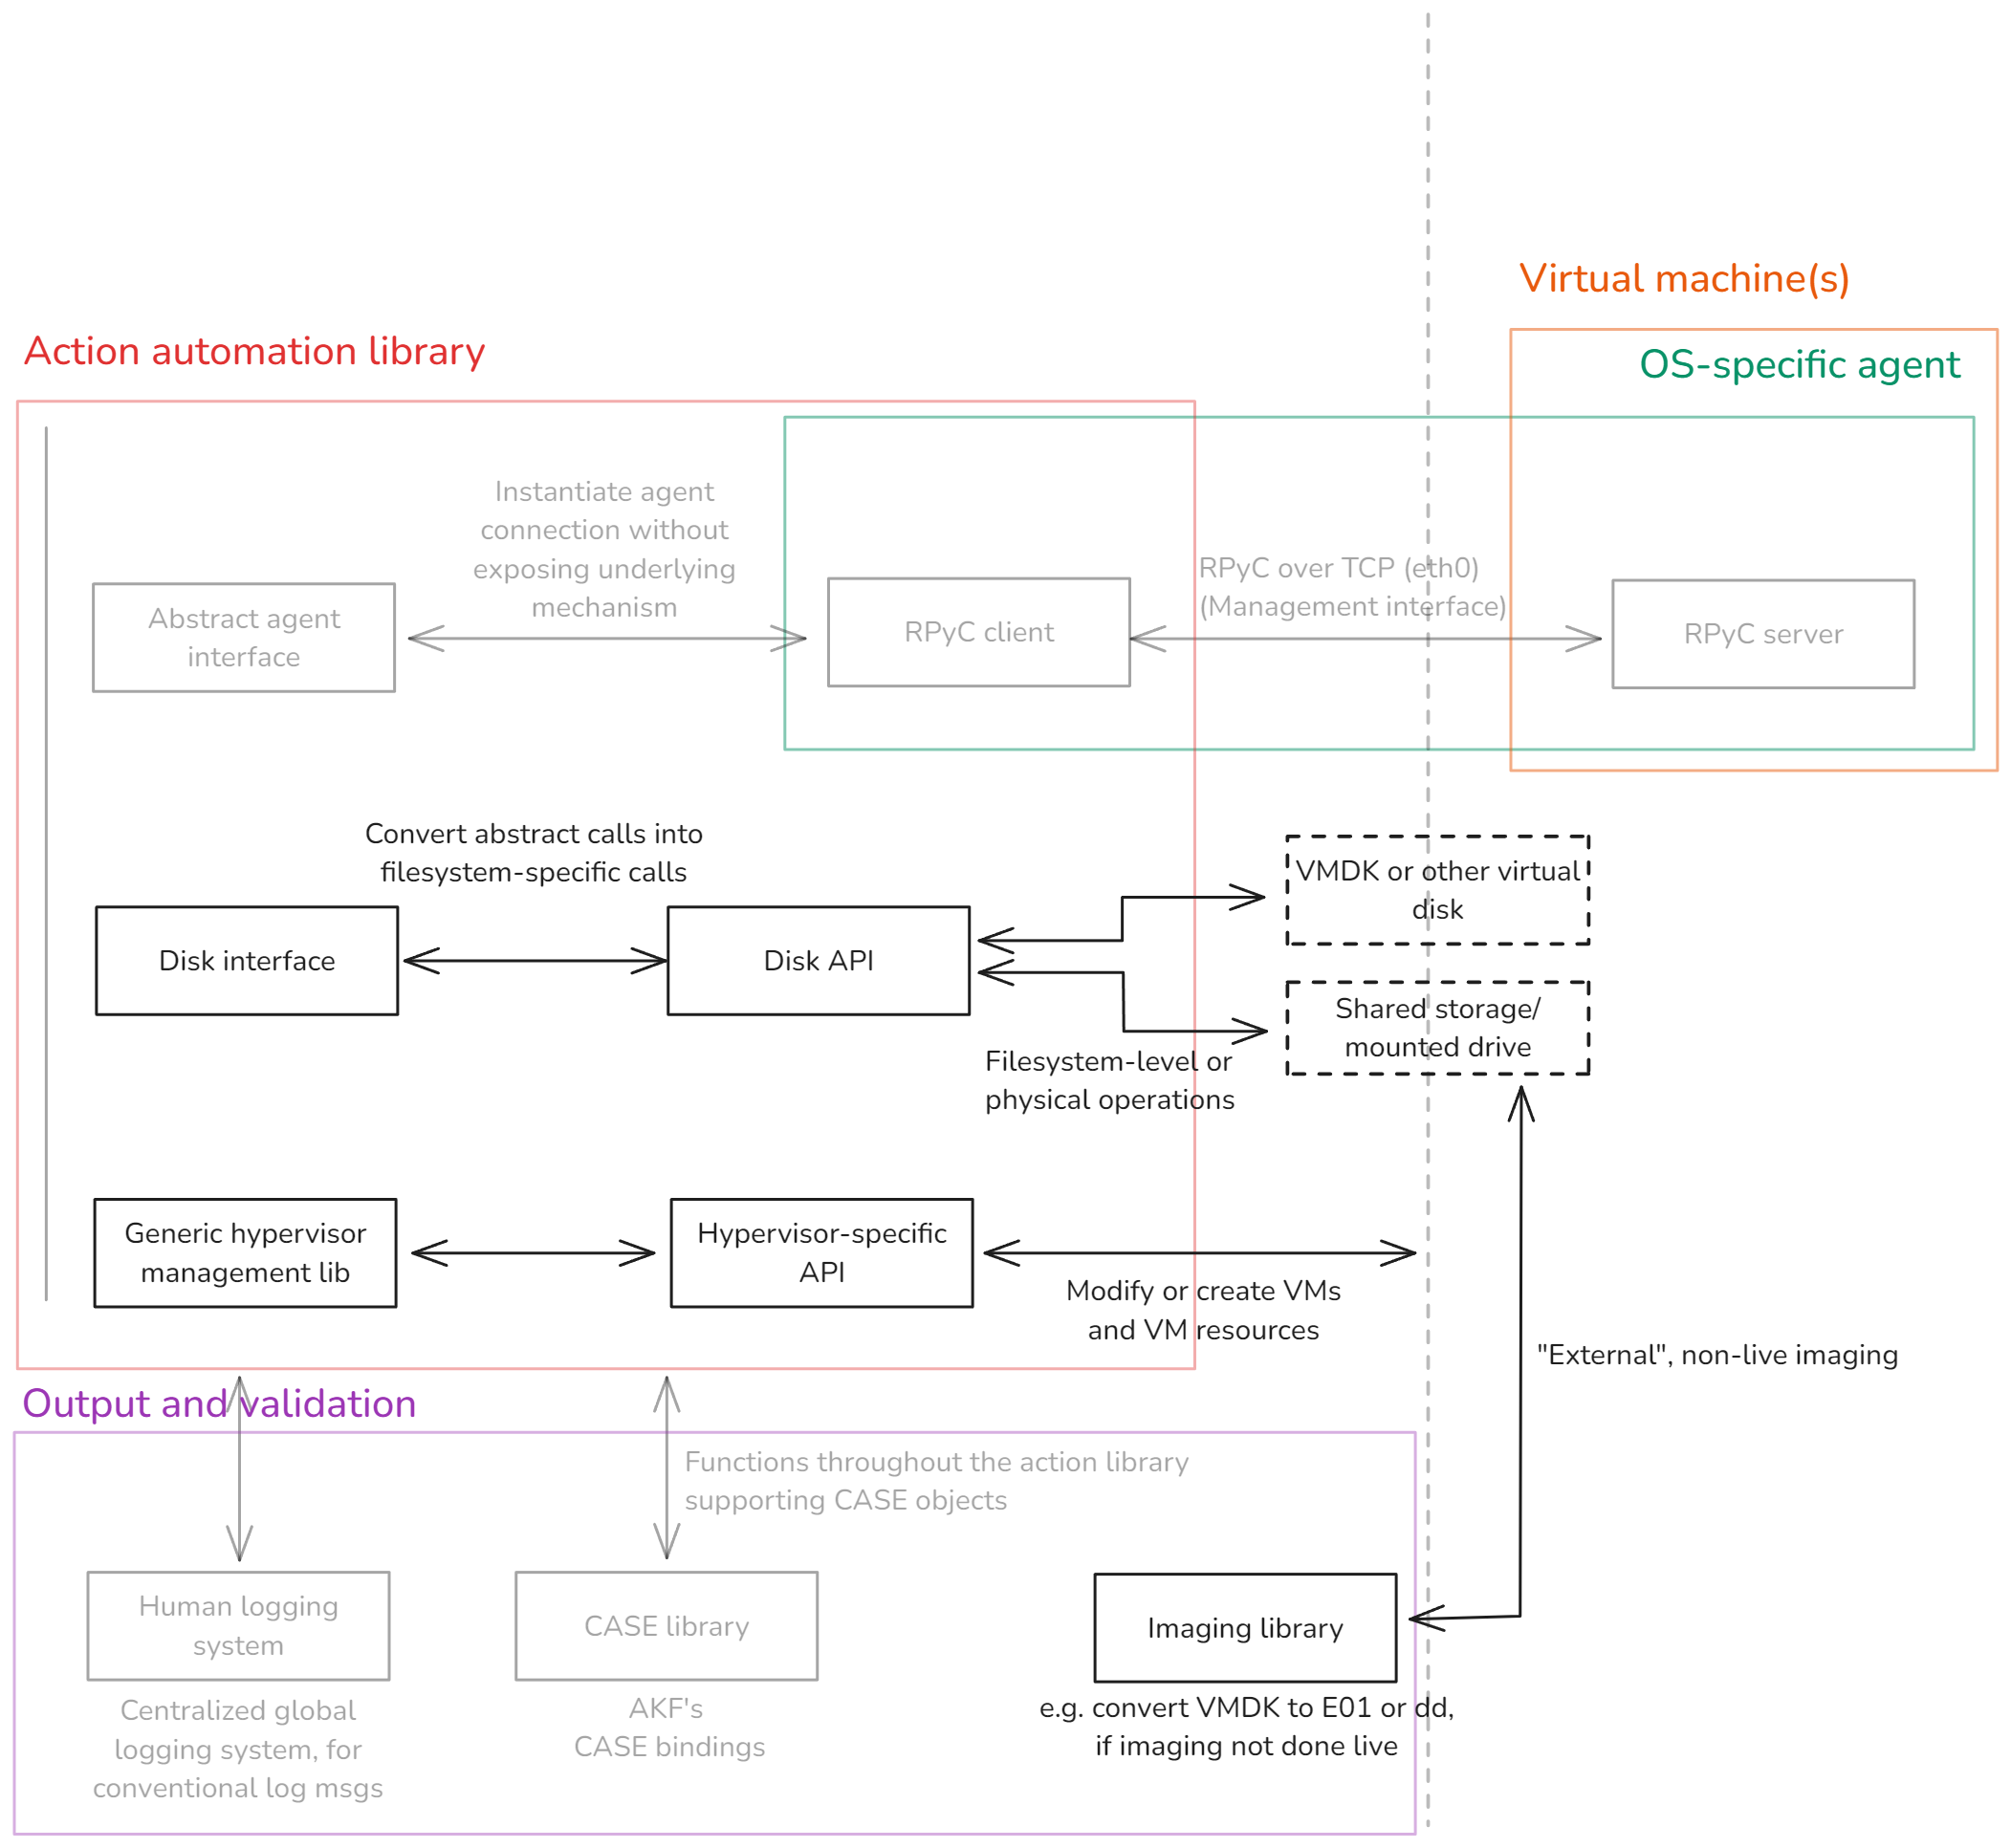
\includegraphics[width=1\linewidth]{action-physical.png}
\caption{Abridged submodule diagram for agent-based artifact
creation}\label{fig:action-physical}
\end{figure}

First, AKF does not currently support mounting and writing to arbitrary
filesystems or disk image formats, though this could be implemented
using external image mounting software with the assistance of
filesystem-independent libraries such as PyFilesystem
\cite{PyFilesystemPyfilesystem22025}. However, AKF allows users to
construct new ISO files from an existing host directory using the
\passthrough{\lstinline!pycdlib!} library
\cite{lalancetteClalancettePycdlib2025}. These ISOs can be used as
standalone artifacts (for example, presenting them to students as disk
images of removable drives) or as removable storage on a running virtual
machine. Mounting these ISOs, as well as setting up a shared network
folder between the host and guest machines, are the simplest means
through which scenario developers can transfer files onto a running
virtual machine.

Second, AKF also trivially ``supports'' filesystem-independent direct
editing. Python allows users to open files in binary mode, at which
point the user can call \passthrough{\lstinline!seek()!} on the file
pointer to advance the pointer to a specific offset in the file. The
user can then call \passthrough{\lstinline!write()!} to overwrite an
arbitrary number of bytes at that position, achieving the same outcome
as many other synthesizers that implement range and offset-based disk
image editing.

Although writing to arbitrary positions is not always viable for
correctly placing artifacts on a disk image, it is still a valid
approach when the underlying filesystem has already been analyzed and
the exact offsets and ranges to write are known. This may be the
approach used by EviPlant \cite{scanlonEviPlantEfficientDigital2017}
to construct and leverage its evidence packages for students; because
filesystem analysis is costly and requires additional libraries not
needed for offset-based editing, it is easier to perform this analysis
at construction time and distribute the offsets to which data must be
written to base images.

However, the filesystem may not have been analyzed ahead of time such
that the exact offsets and data needed to place a file on disk are
known. This brings us to filesystem-aware direct editing, in which AKF
makes significant improvements.

ForGe implements its physical artifact generation by implementing NTFS
and FAT32 data structures in Python, allowing it to create a fully
virtual representation of these filesystems (with the assistance of a
custom C program). This virtualized filesystem provides ForGe with the
information necessary to efficiently insert data into known slack and
unallocated space while maintaining filesystem consistency. While
extremely powerful (and implements a valuable feature not found in any
other synthesizer to date), it is inflexible in two specific aspects:

\begin{itemize}
\tightlist
\item
  ForGe does not provide a generic interface for the filesystems it
  supports. Although the NTFS and FAT32 wrappers provide the same
  methods with the same signatures, this is not strictly enforced by a
  parent class. The lack of a generic interface means that the
  functionality supported across all filesystems is unclear, as is the
  functionality that must be implemented for new filesystems to be
  compatible with ForGe.
\item
  ForGe lacks a ``frontend'' to support arbitrary disk types, regardless
  of the underlying filesystem. ForGe does not support multi-partition
  disks or common non-raw disk formats such as VHD, VMDK, or VDI.
\end{itemize}

Read-only libraries addressing these two issues have been in development
since the introduction of ForGe but have not been integrated into other
synthesizers to achieve the same write capabilities as ForGe. One such
library is \passthrough{\lstinline!libtsk!} (also known as The Sleuth
Kit), the C++ library that powers the open-source digital forensics
software Autopsy \cite{SleuthkitSleuthkit2025}.
\passthrough{\lstinline!libtsk!} allows users to navigate and analyze
the low-level contents of a variety of filesystems, including
filesystem-specific attributes and the sequence of disk clusters that
form a file. \passthrough{\lstinline!libtsk!} supports a large variety
of filesystems through a filesystem-agnostic interface, including the
FAT family of filesystems, the ext family, NTFS, and a variety of other
filesystems. ~It also supports various volume systems for
multi-partition disks, such as GPT and MBR, as well as several
filesystem containers and images.

Python bindings for \passthrough{\lstinline!libtsk!} have existed for at
least 15 years, with the most commonly used library being the
automatically generated \passthrough{\lstinline!pytsk!}
\cite{Py4n6Pytsk2025}. However, \passthrough{\lstinline!pytsk!} has
relatively limited Python documentation and adoption, in addition to
inheriting various known issues and limitations in
\passthrough{\lstinline!libtsk!}, such as support for niche filesystems
and partitioning formats. Many of these gaps were gradually covered as
part of the \passthrough{\lstinline!libyal!} project, a collection of
DFIR libraries developed by various contributors - most notably Joachim
Metz from Google \cite{LibyalLibyal2025}. The
\passthrough{\lstinline!libyal!} project includes individual libraries
for analyzing formats not supported by \passthrough{\lstinline!libtsk!},
such as the QCOW disk image format used by QEMU, the Apple File System
used by modern Apple devices, and more.

These libraries eventually led to the development of
\passthrough{\lstinline!dfvfs!}, or the Digital Forensics File System, a
Python library that leverages \passthrough{\lstinline!libtsk!} and
multiple libraries from the \passthrough{\lstinline!libyal!} project to
provide a generic interface for analyzing a variety of disk image
formats and filesystems \cite{Log2timelineDfvfs2025}. (The project
is derived from Plaso and Google Rapid Response, two open-source DFIR
tools used in various contexts.) Much like
\passthrough{\lstinline!libtsk!}, it exposes a variety of low-level
filesystem concepts common across multiple filesystems, such as the
metadata and individual segments comprising a file at a known path on
the filesystem. This low-level detail makes it extremely powerful in
performing filesystem-aware direct editing, especially because of its
focus on exposing this detail through a consistent Python interface.

AKF uses \passthrough{\lstinline!dfvfs!} to locate the clusters of a
file at a known path in a filesystem, which can then be used to identify
the start of slack space within the file's clusters (as well as
unallocated space in the filesystem). By adding the physical offset of
the cluster within the filesystem to the offset of the filesystem's
partition in the disk image, AKF can write to the exact location of a
file's slack space using the offset-based method described earlier. This
achieves feature parity with ForGe, completely delegating filesystem and
image-specific details to \passthrough{\lstinline!dfvfs!} and allowing
for a filesystem-independent method for locating slack space.

More generally, this technique provides a deterministic method for
inserting data within the slack space of a filesystem, simulating the
deallocation of a file and its partial replacement with a known file.
However, this does not fully simulate the process of deleting a file
through a running operating system and having a new file replace the
deallocated clusters; naturally, this does not generate OS-specific
artifacts associated with deleting and creating files and fails to
generate the filesystem artifacts that could exist with the original
file (such as the ``deleted'' file's name in the NTFS master file
table). Future work in the field could address this gap by combining
\passthrough{\lstinline!dfvfs!} with additional technologies to improve
the accuracy of physical techniques.

It should be noted that this technique does not work on filesystems with
full disk encryption enabled, as is the default on Windows systems
beginning with the Windows 11 24H2 update. Additionally, this technique
has only been verified to work on raw disk image formats. From limited
testing, the offsets of partitions and files on compacted formats such
as VHD are reported by \passthrough{\lstinline!dfvfs!} as if the
partition were not compact, which makes it difficult to correctly
determine the physical offset of a file on a VHD image. Additional
research is needed to develop a reliable method for performing
filesystem-aware physical artifact generation on such disk image
formats.

\chapter{Output and validation}\label{chapter-five}

\hfill\break

This chapter addresses the mechanisms through which AKF generates and
documents its outputs, as seen in \autoref{fig:output-simple}. More
specifically, this covers the modules and submodules seen in
\autoref{fig:output-full}. The submodules for the \emph{virtual machine}
and \emph{action automation library} have been omitted for brevity.
(Note that the ``imaging library'' and ``validation library'' are
theoretical submodules that would fulfill the ``after the fact''
analysis described in \autoref{human-readable-reporting}, and are not currently implemented.)

\begin{figure}[h]
\centering
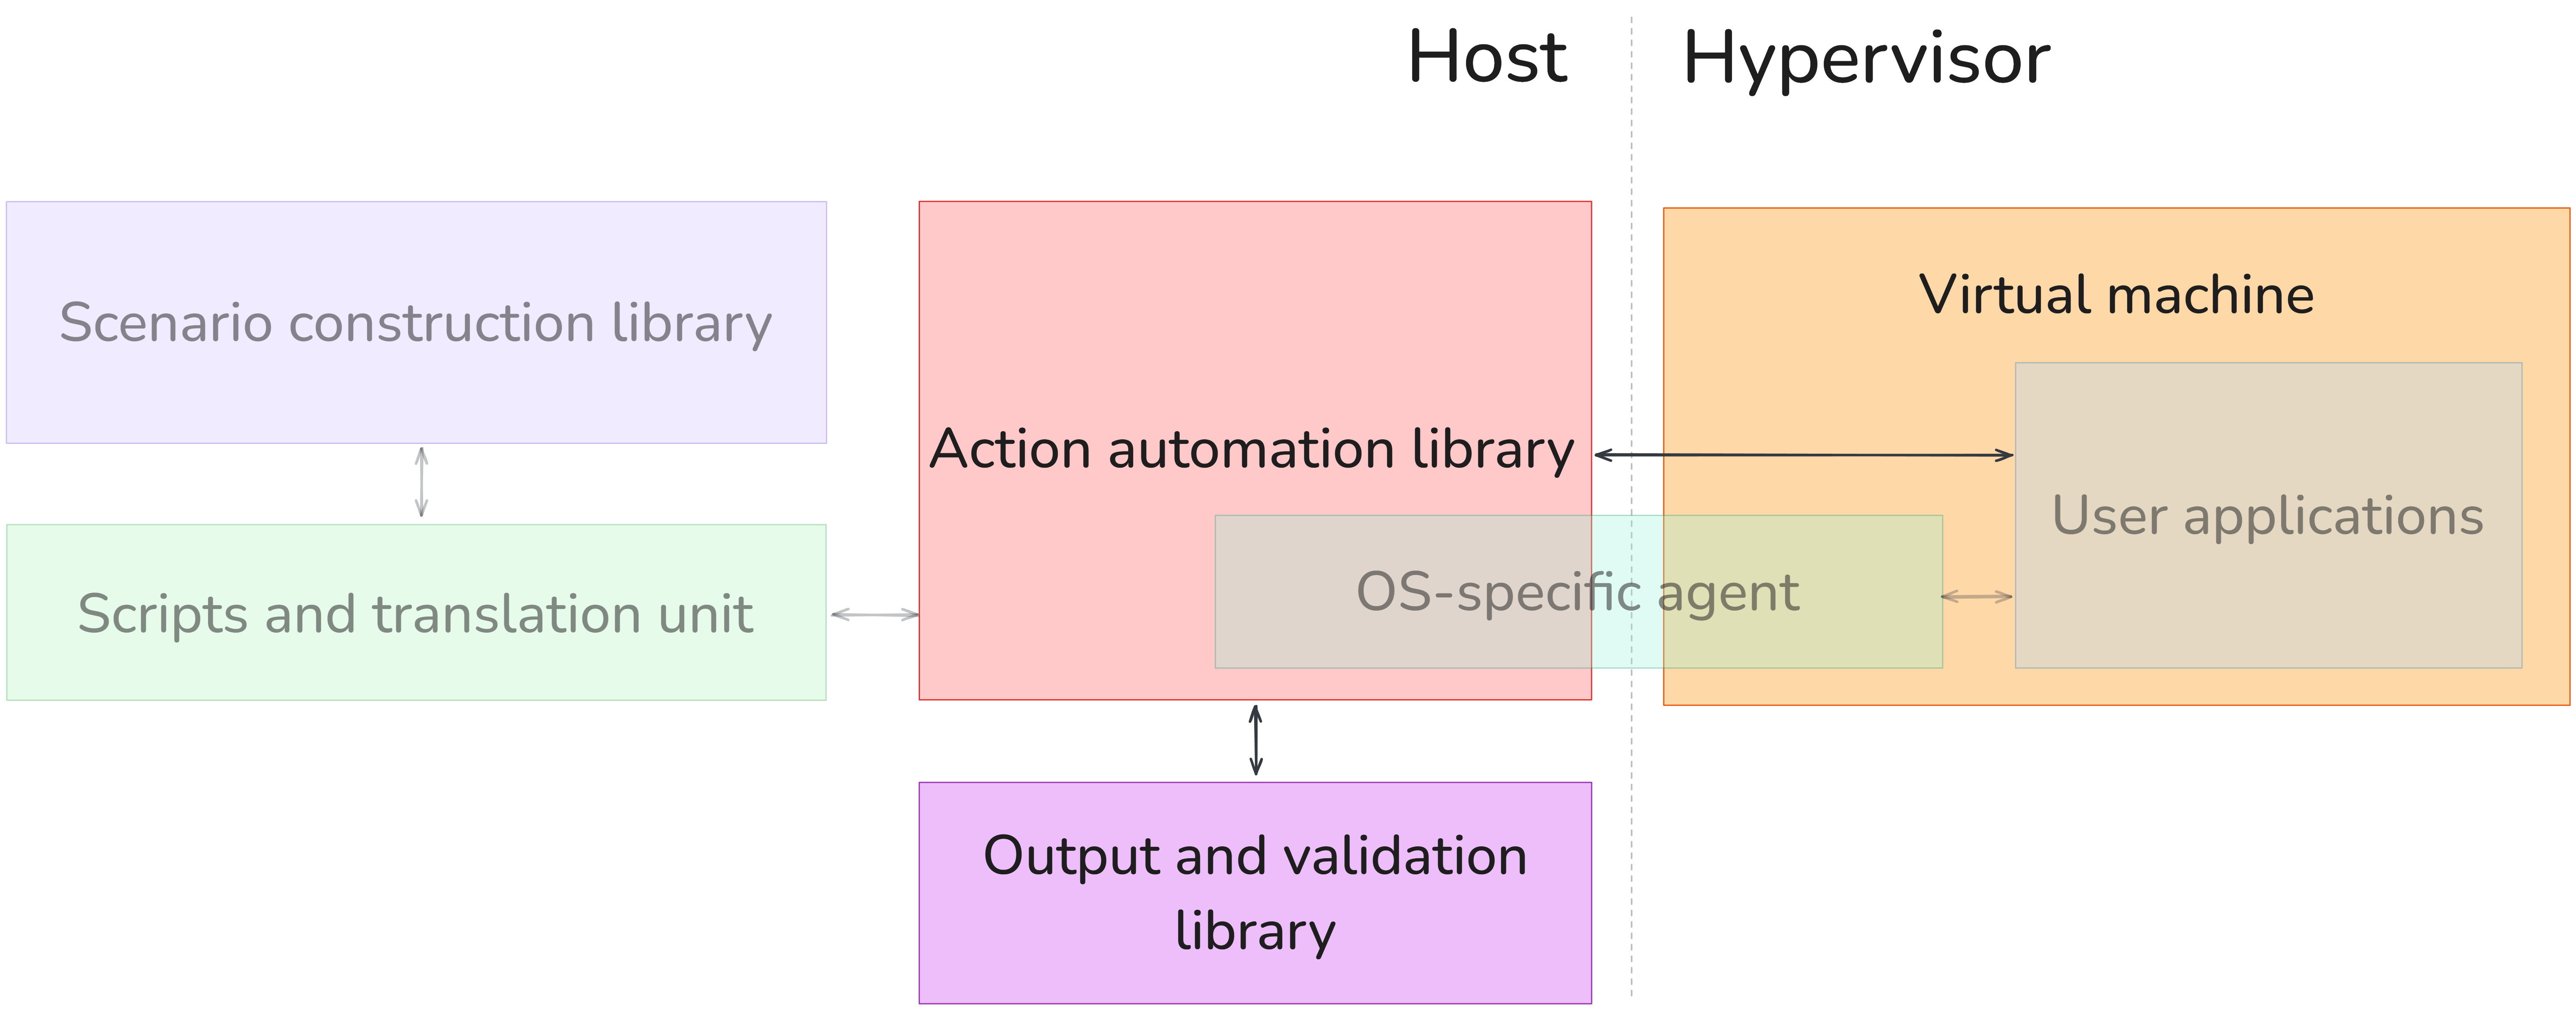
\includegraphics[width=1\linewidth]{output-and-validation-simple.png}
\caption{Simplified AKF architecture diagram for output and validation
modules}\label{fig:output-simple}
\end{figure}

\begin{figure}[h]
\centering
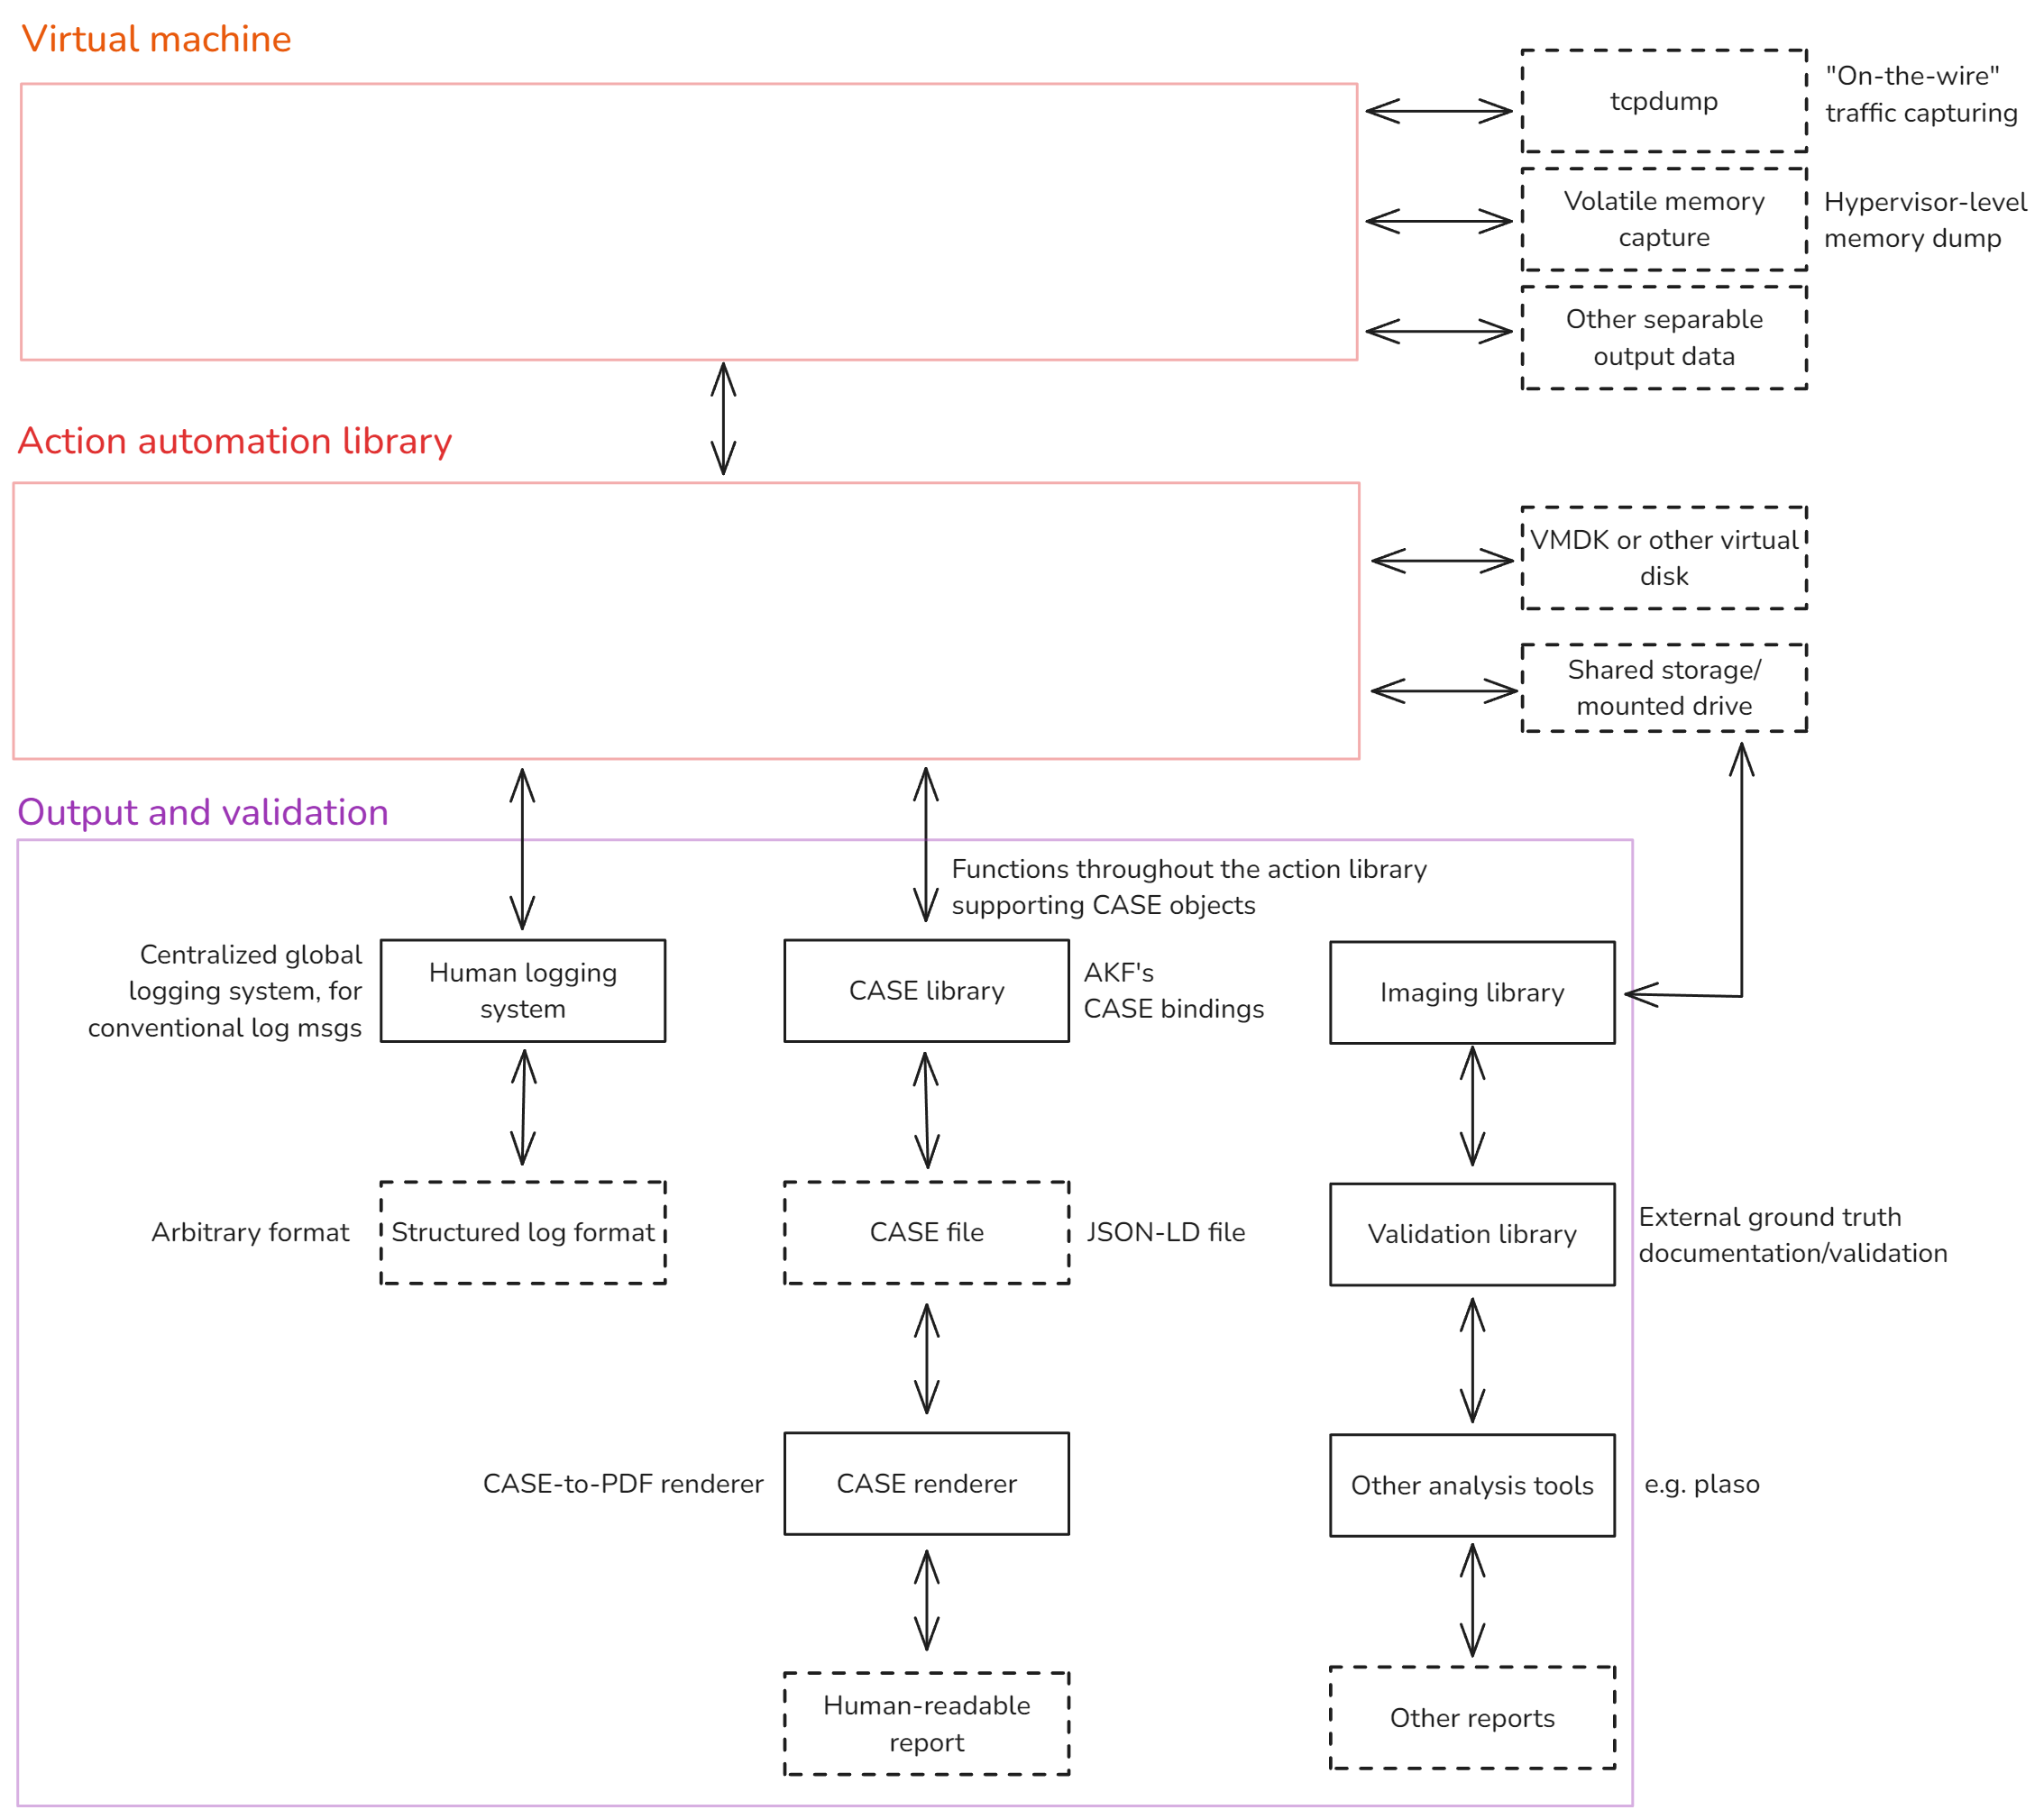
\includegraphics[width=1\linewidth]{output-and-validation-full.png}
\caption{Abridged diagram of AKF modules related to output and
validation}\label{fig:output-full}
\end{figure}

Whether generating artifacts through physical or logical means, these
artifacts must ultimately be exported and documented. In most cases,
this involves generating disk images, volatile memory captures, or
network captures; additionally, individual artifacts, such as browser
history, may be selectively extracted from a filesystem. Disk, memory,
and network captures will be referred to as ``core outputs'' throughout
this chapter to distinguish them from ``standalone'' artifacts. Both can
be broadly described as ``outputs'' of a scenario.

The contents and details of these artifacts, as well as the means
through which they were generated, should be documented in a structured
format. This ground truth should fully describe the contents of a
forensic dataset; that is, it should identify every artifact that can be
discovered within a dataset and every action taken to plant those
artifacts. This metadata, in addition to core outputs and standalone
artifacts, comprises a forensic dataset.

From an educational perspective, the ground truth represents an ``answer
key'' to the dataset; it details every artifact of interest that an
analyst could be expected to discover. For research, it allows for
well-labeled datasets that can be used for tool development, validation,
and testing. Ideally, this should be generated independently of the
input script used to construct the scenario. This allows \emph{all}
artifacts to be documented, including those not explicitly declared or
deemed significant by the scenario creator.

This chapter addresses the role of the output and validation library in
providing several AKF services, including a centralized logging system,
CASE object generation, and the generation of outputs such as disk
images, network captures, and volatile memory dumps. In particular, it
describes the reporting and documentation functionality enabled by CASE
and the role that this metadata plays in ensuring dataset
reproducibility and supporting community usage.

\section{Core outputs}\label{core-outputs}

In the same way that artifacts can be generated through logical and
physical means, outputs can also be generated through logical and
physical means. Some of these are analogous to techniques used by
real-world investigators to extract forensically sound evidence that is
valid in a court of law; others are less suitable in formal settings but
still have valid use cases.

Logical output generation refers to any technique in which software is
used inside a running virtual machine to generate these outputs. This
includes using software such as FTK Imager
\cite{exterroFTKImagerForensic} to capture the volatile memory of a
device or construct a \emph{logical} disk image. Similarly, network
captures can be created by simply running Wireshark on the target
device. Individual artifacts can be copied off the device by hand and
sent to a network or removable drive.

Physical output generation refers to techniques in which the operating
system is unaware of the technique, leaving few or no traces in the
resulting outputs. In practice, this involves using tools such as
hardware write blockers to extract disk images and network taps (or
another traffic mirroring solution) to capture traffic over a particular
interface. Although challenging, a physical extraction of RAM is also
possible by performing a ``cold boot attack.'' RAM sticks can be cooled
to low temperatures before being removed from a running machine, slowing
the process of memory decay as a result of the DRAM cells being
unpowered \cite{yitbarekColdBootAttacks2017}.

AKF directly supports physical output generation for all three core
outputs and indirectly supports logical output generation for core
outputs and standalone artifacts. Physical output generation for virtual
machines is generally achieved through direct interaction with the
hypervisor.

\begin{itemize}
\tightlist
\item
  For \textbf{disk images}, the output can simply be the virtual hard
  drive used by the hypervisor on the host machine (such as VDI files
  for VirtualBox). If a standard raw disk image is desired, the
  command-line tool VBoxManage supports converting various virtual drive
  formats to raw disk images using the
  \passthrough{\lstinline!vboxmanage clonemedium!} command. This expands
  the compacted virtual drive to the ``declared'' size of the drive as
  seen by the operating system, allowing it to be bootable on actual
  hardware.
\item
  For \textbf{network captures}, VirtualBox allows the user to enable
  network tracing over multiple interfaces, dumping network traffic as a
  .pcap file on the host machine. This can be enabled or disabled at any
  time without affecting network connectivity or the state of the
  virtual machine.
\item
  For \textbf{volatile memory dumps}, VBoxManage provides the command
  \passthrough{\lstinline!vboxmanage debugvm <machine\_name> dumpvmcore!},
  which creates an ELF core file of the virtual machine's volatile
  memory that can be analyzed using a tool such as Volatility
  \cite{volatilityfoundationVolatility32025}.
\end{itemize}

These physical output options are often sufficient to generate datasets.
If only specific files are desired, the existing file transfer utilities
provided by AKF can be used to extract standalone artifacts. Users can
also manually perform the logical techniques described above (such as
running Wireshark or installing FTK Imager) through various means. For
example, a user can pause an AKF script until instructed to continue;
during this time, the user can manually run FTK Imager to extract the
contents of RAM.

The logic for generating physical outputs is contained in the opaque
submodules seen in \autoref{fig:output-a}.

\begin{figure}[h]
\centering
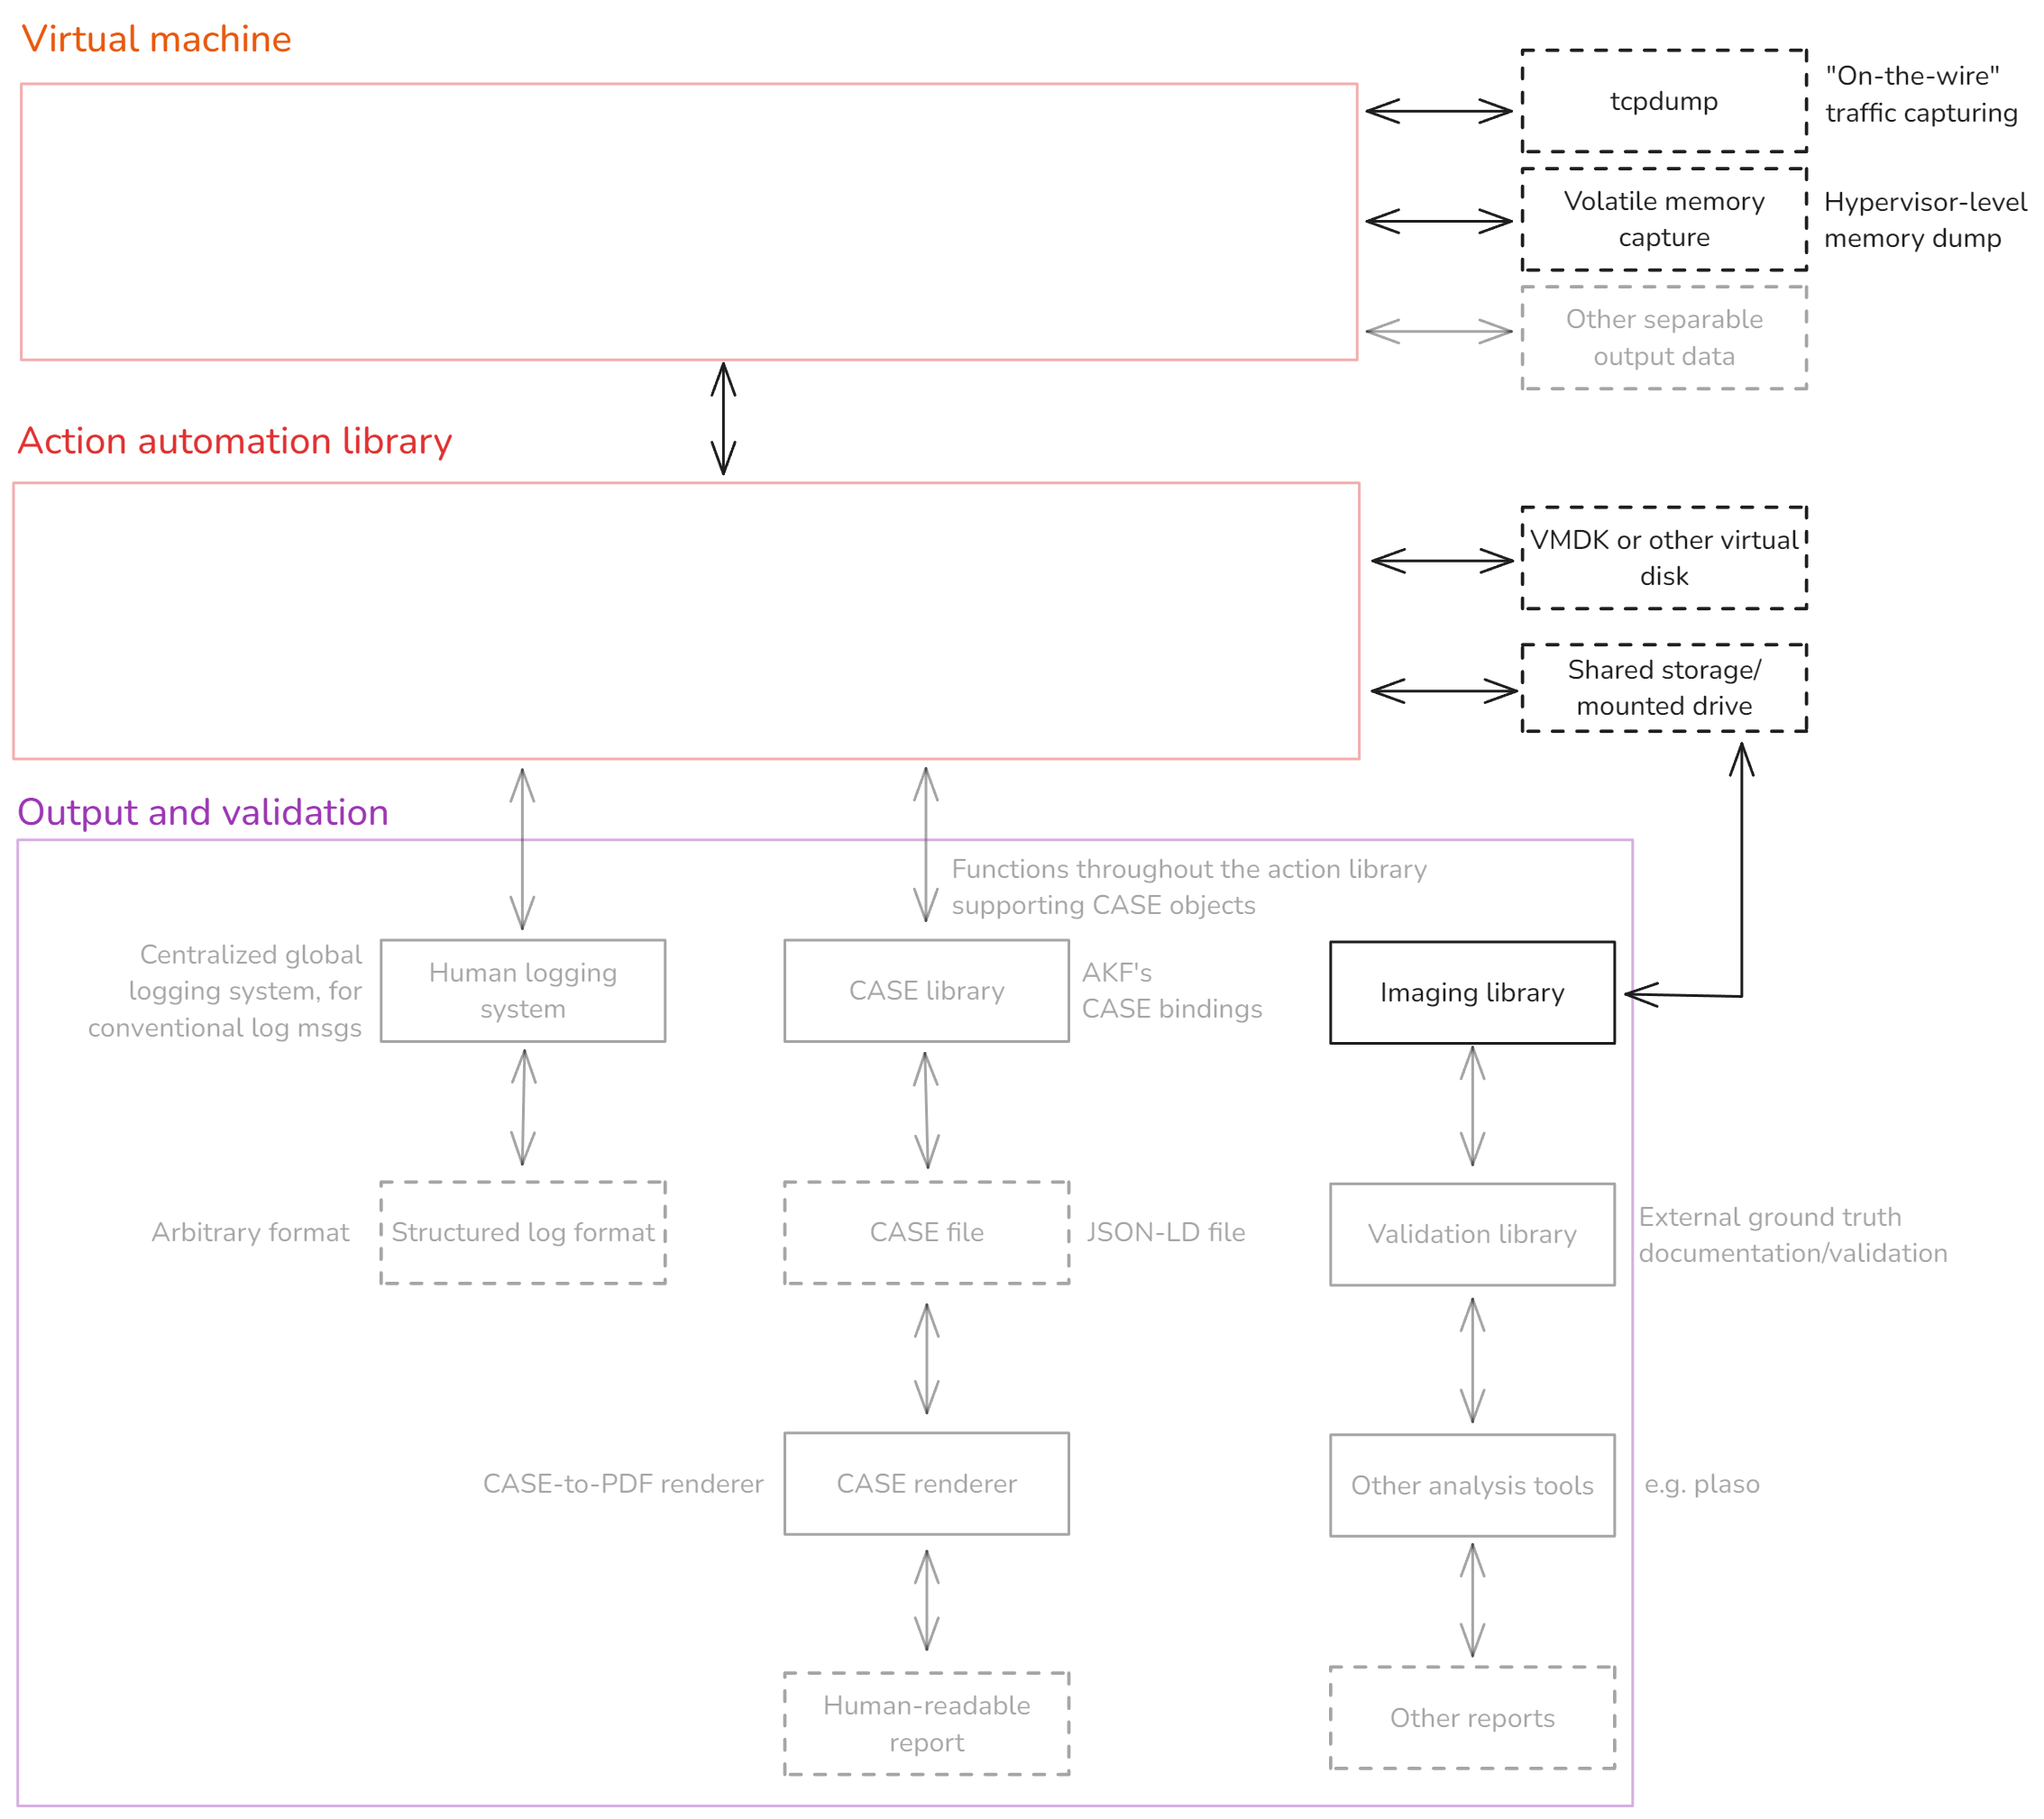
\includegraphics[width=1\linewidth]{output-and-validation-a.png}
\caption{Diagram of AKF modules related to physical output
generation}\label{fig:output-a}
\end{figure}

\section{Metadata and ground
truth}\label{metadata-and-ground-truth}

There exists a gap in the ability of instructors and researchers to
perform bulk searches for specific forensic artifacts in public
datasets. For example, the NIST CFReDS repository
\cite{nationalinstituteofstandardsandtechnologyCFReDSPortal}, one of
the largest listings of forensic datasets, does not have a unified
standard for describing uploaded images. Although users can search by
keywords and human-applied tags, metadata is not available in a
standardized format.

For many datasets, an instructor or researcher must read through a PDF
answer key (if one exists) or analyze the image themselves to determine
if a particular artifact is present. Answer keys are not inherently
machine-readable and are not suited for identifying specific artifact
types in bulk. Additionally, the content of human-made reports may be
limited to what the author believes is significant, even if other
artifacts of interest are present in the image. In turn, it may be
difficult to quickly determine if a dataset is useful in demonstrating a
particular technique to students or validating a specific feature of a
newly developed tool.

A rigid, well-defined format for ground truth is invaluable to
researchers engaging in tool validation and development. Perhaps the
lack of labeled forensic datasets on major repositories can be
attributed to the lack of a need for one; Grajeda et al.~demonstrated
that scenarios are rarely shared between researchers, so there is seldom
a need to label them for general-purpose usage. AKF has the opportunity
to solve this issue through the mass production of labeled datasets
adopting a single established standard.

Many forensic analysis tools support exporting investigation details in
both proprietary and language-agnostic formats, though these are not
always suitable for generating ground truth. For example, Cellebrite's
UFED supports exporting to UFDR and XML files, Magnet Axiom supports
exporting to XML, and Autopsy supports a variety of formats, including
Excel, STIX, and HTML. Each format varies in structure and content and
does not necessarily contain equivalent information for the same
analyzed disk image using default settings. This is the primary
challenge with using an existing format, particularly a proprietary
format subject to vendor changes; details for certain artifact types may
be missing or change without warning. Many prior synthesizers (including
AKF) also generate human-readable log messages during artifact
generation, though this is rarely suitable for documenting the contents
of a dataset.

There has been extensive work in other fields towards developing a
structured ontology that describes relationships and low-level details.
This includes the EVIDENCE project for criminal justice and the
Structured Threat Information Expression (STIX) format for conveying
cyber threat intelligence
\cite{caseyLeveragingCybOXStandardize2015}. For example, STIX
provides a standard set of objects that allows organizations to describe
observed attacker techniques and associate them with specific pieces of
malware, attack campaigns, or threat actors.

However, there have been few efforts to document the contents of a
forensic scenario (disk images and related metadata) in a vendor-neutral
manner. One such format was developed by Abbott et al., who provide an
XML-based notation of events in a dataset
\cite{abbottAutomatedRecognitionEvent2006}. However, the
specification does not appear to be available or maintained as part of
another project. Similarly, although not designed to document technical
details in a dataset, Conlan et al.~describe a taxonomy for describing
anti-forensic techniques at a high level that could be integrated into a
scenario description language
\cite{conlanAntiforensicsFurtheringDigital2016}. Neither of these
formats appear to be supported by community tools, nor do they fill the
need for low-level, queryable dataset descriptions.

Besides limited community support for and adoption of existing formats,
Casey et al.~found that these formats lacked features such as
parent-child relationships, user actions, and non-technical case
information such as a chain of custody. In response, the same authors
introduced the Digital Forensic Analysis eXpression, or DFAX, a language
extending CybOX (the predecessor to STIX) for use in the digital
forensics community. DFAX later became the Cyber-investigation Analysis
Standard Expression (CASE)
\cite{caseyAdvancingCoordinatedCyberinvestigations2017}. CASE is
perhaps the most comprehensive and actively supported ontology available
for digital forensics; contributors include NIST with support from the
Linux Foundation. As a result, AKF uses CASE as its primary format for
documenting datasets, deliberately including support for CASE throughout
various libraries.

\subsection{CASE and Python
bindings}\label{case-and-python-bindings}

CASE is a vendor-neutral format designed to document both technical and
non-technical information about a digital forensics case
\cite{caseyAdvancingCoordinatedCyberinvestigations2017}. It aims to
cover as many OS-specific and application-specific artifacts as possible
while still providing the flexibility to describe artifacts from
uncommon applications. In theory, data exported from any major vendor,
such as Cellebrite, Magnet, or FTK, can be converted into a valid CASE
file. CASE is an extension of the Unified Cyber Ontology, or UCO, which
provides basic objects not specific to digital forensics (such as
applications or users). Consistent with the CASE project's
documentation, references to CASE and CASE/UCO throughout this chapter
refer to the same project.

CASE is built on the Resource Description Framework (RDF), a model for
describing information using relationships. Two objects are linked using
a predicate, with the set of three elements forming a ``triple.'' This
pattern allows for directed, labeled graphs to be expressed using RDF.
The ontology of CASE objects is defined using the Terse RDF Triple
Language, or Turtle, which allows these triples to be written in a
simple text format. In many ways, the Turtle definitions can be seen as
the class definitions for CASE objects; instances of these objects can
be expressed in JSON-LD, an extension of JSON for linked data. A
collection of CASE objects is known as a bundle; applications can add
instantiated CASE objects to a bundle as needed.

Because the CASE format itself is language-agnostic, it is necessary to
write language-specific libraries that allow for instantiating CASE
objects. At the time of writing, the CASE project provides Python
bindings for UCO/CASE version 1.4 \cite{CaseworkCASEMappingPython}.
Each unique object type is represented as a Python class, which can be
instantiated to produce individual objects. However, this library has
several limitations due to its design; for example, CASE objects are
internally represented as a dictionary of strings rather than a set of
instance variables. While this makes it easier to serialize CASE objects
to JSON-LD dictionaries, modifying objects after they have been
instantiated is extremely difficult.

It is also worth noting that each object in the CASE ontology appears to
have been manually translated to its corresponding Python class
definition. This is slow and time-consuming, especially given that a
significant overhaul of UCO/CASE to version 2.0 is underway with new
object definitions \cite{UcoProjectUCODevelop2002025}; there appears
to be no active effort to update the 1.4 bindings to 2.0.

AKF leverages and contributes Pydantic-based bindings for CASE. The
foundation for this system is the Pydantic library for Python, which
allows developers to quickly define classes (referred to as ``Pydantic
models'' or simply ``models'') with built-in schema validation and
serialization based on Python type hints \cite{colvinPydantic2024}.
More broadly, Pydantic allows us to simplify the declaration of
individual objects while providing runtime type validation and automatic
casting.

Examples of CASE-related definitions and a detailed comparison of AKF's
bindings compared to the existing CASE bindings can be found in
\autoref{case-python-bindings}. One notable example
from this section is the simplification of a CASE object declaration
from 35 lines in the existing CASE bindings to only three lines in AKF.
These simple declarations are possible primarily because the conversion
of objects to valid JSON-LD elements is deferred until serialization
instead of converting objects to dictionaries immediately upon
instantiation. This design choice allows us to centralize the
serialization logic in a single parent class that all CASE objects
inherit from. In exchange for slightly increasing the complexity of
converting objects to a dictionary with the correct key names, we can
massively simplify the logic for declaring individual CASE objects.

A script is provided with AKF's CASE bindings to automatically parse the
RDF files and convert them to valid Pydantic models. It automatically
converts XSD datatypes to their native Python types (or a custom wrapper
type if a native type does not exist), correctly inherits classes, and
automatically generates docstrings and Pydantic fields as applicable.
The script also topologically sorts dependencies in the same file; an
RDF object's ``parent'' class may be declared \emph{after} its ``child''
class, which is disallowed in Python. This dramatically simplifies the
process of maintaining Python bindings for UCO/CASE, as well as the
overall design of the library for future needs.

Note that there are certain inconsistencies between the Turtle CASE
definitions and those of AKF. These issues are true of the public
bindings for CASE/UCO 1.4 that are currently available, as well; this is
not unique to AKF's Pydantic-based implementation. These are described
in greater detail at the end of \autoref{case-python-bindings}.

\subsection{CASE integration in
AKF}\label{case-integration-in-akf}

AKF's CASE Python bindings are integrated throughout artifact-generating
libraries in AKF. This is depicted through the opaque submodules in
\autoref{fig:output-b}.

\begin{figure}[h]
\centering
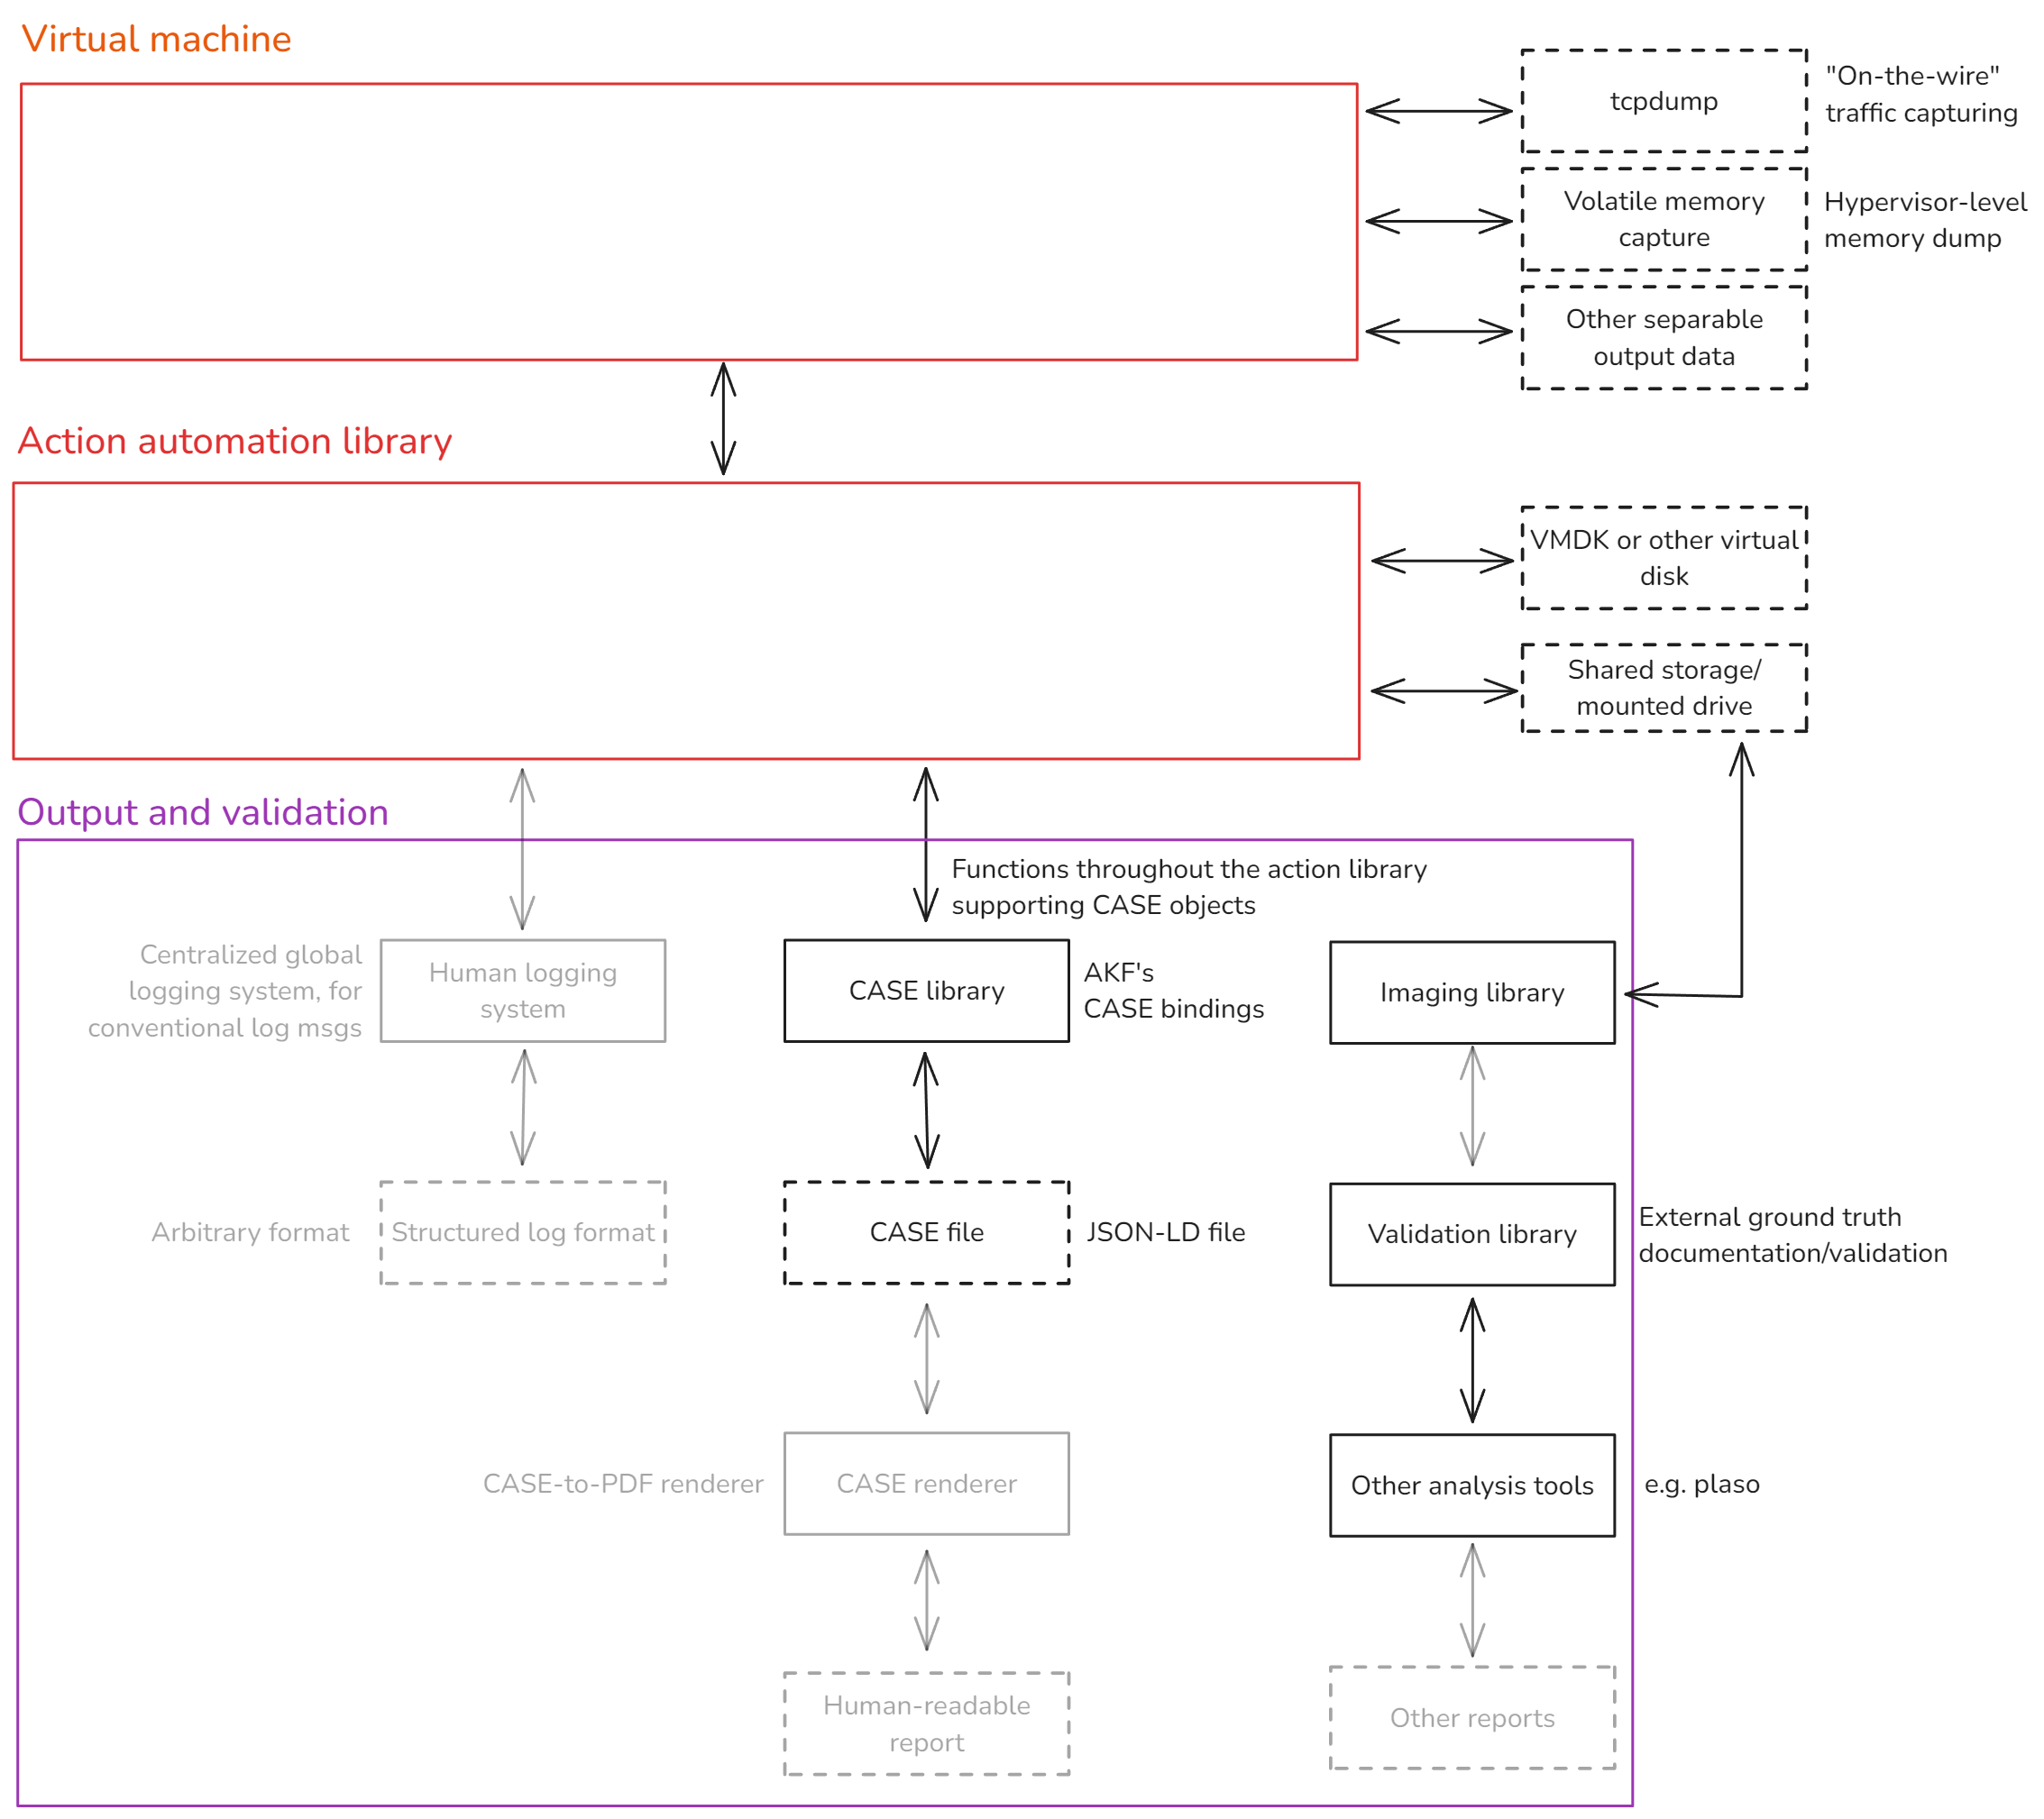
\includegraphics[width=1\linewidth]{output-and-validation-b.png}
\caption{Diagram of AKF modules related to CASE object
generation}\label{fig:output-b}
\end{figure}

There are two distinct points at which CASE artifacts can be generated
and attached to a scenario -- during scenario generation and after
scenario generation.

Various functions and classes throughout the AKF core libraries and
agent API accept an optional CASE bundle when invoked or instantiated.
As users call CASE-compatible functions, these functions can
automatically add CASE objects corresponding to the artifacts generated
through their execution. For example, if the agent subservice API for
automating Chromium browser actions is provided with a CASE bundle,
navigating to a page using the API could automatically generate a CASE
object describing the page visit and add it to the bundle. This process
can occur entirely within the host, allowing CASE-related logic to
remain out of the agent where needed.

However, recall from \autoref{the-akf-agent} that using RPyC for agent communication allows AKF to pass
complex objects between the agent and the host machine. This includes
CASE bundles and objects, as well. For example, suppose that a CASE
object must be made for a file downloaded from the internet that
frequently changes location, size, and content. The resulting CASE
object can only be accurately constructed using some form of agent-side
analysis as the action occurs. Once instantiated, the object can be
returned to the host machine to append to a larger CASE bundle.

Some CASE ontology objects, such as those describing Windows prefetch
files, are best constructed when disk images and other core outputs are
created. For example, it is possible to create CASE prefetch objects
during the execution of a scenario. However, these objects are likely to
become outdated if their corresponding applications are launched later
in the scenario, thus changing the content of the prefetch files and
making the existing CASE objects inaccurate.

In turn, to make the generation of such objects more efficient and
accurate, certain CASE objects must be instantiated ``after the fact'';
that is, they cannot or should not be automatically generated as part of
AKF automation routines. This can be trivially achieved by analyzing
core outputs (such as disk images) using independent tooling. Such tools
might include general-purpose DFIR tools that support CASE objects (such
as Autopsy) or tools that explicitly focus on constructing CASE objects
(such as tools built with the official or AKF Python bindings for CASE).

However, ``after the fact'' analysis can also be achieved on live
virtual machines using existing AKF design patterns. In particular,
agents may have RPyC subservices whose sole purpose is to generate CASE
objects. For example, the \passthrough{\lstinline!artifacts!} subservice
mentioned in \autoref{the-akf-agent}
can collect Windows prefetch files immediately before a disk image is
created, allowing it to construct CASE prefetch objects that reflect the
disk image without requiring separate tooling. CASE-oriented
functionality can also be implemented in existing subservices; for
example, the \passthrough{\lstinline!chromium!} subservice can create
CASE objects for Chrome and Edge browser history after all browser
automation actions have been performed. This allows the dataset to be
documented independently of synthesizer actions intended to emulate
human activity -- a desirable feature identified at the beginning of
this chapter.

The flexibility of these two approaches -- enabled by CASE's deep
integration into AKF -- makes it possible to construct CASE objects in a
manner that requires little additional effort by scenario developers.
Scenario developers do not need to be concerned with instantiating their
own CASE objects when using high-level APIs so long as an AKF library
developer has written support for automatic CASE object construction.
This significantly reduces the need for scenario developers to construct
ground truth information by manually analyzing synthesizer-created
outputs.

By extension, this means that the detailed documentation of AKF outputs
is innate to many scenarios constructed using AKF. Lowering the effort
required to document an AKF-generated scenario improves the likelihood
that any public AKF scenario can be immediately valuable (or determined
to be valuable) to researchers and educators. This significantly
contributes to AKF's goal of supporting an ecosystem around its images;
the CASE bundles of many scenarios can be queried in bulk to identify
datasets that might be useful for a specific purpose without having to
download the dataset itself. This information can also be used to
identify and analyze broader trends across scenarios, such as the
frequency of a particular artifact appearing in all Windows datasets.

While this machine-readable reporting significantly improves the ability
of the forensic community to locate useful datasets, it is verbose and
unsuitable as a human-readable summary. Human-readable reporting is
particularly relevant in a classroom setting, where the distribution of
simplified answer keys to graders and students focusing on key artifacts
is preferable to the exhaustive reporting provided by a CASE bundle.
This leads us to the following section, which briefly addresses the
conversion of AKF-generated metadata into human-readable reports.

\section{Human readable reporting}\label{human-readable-reporting}

As alluded to in the previous section, converting a rigid, well-defined
format to a human-readable format is often easier than performing the
reverse operation. Indeed, this is the approach taken by AKF, which does
not create human-readable reports as an immediate output of dataset
generation. (AKF generates human-readable log files during artifact
generation, but these are unstructured and are created primarily for
debugging rather than analysis.) Instead, AKF supports a simple yet
flexible system for generating human-readable PDF reports from existing
CASE bundles after generating a dataset.

AKF implements human-readable reporting through a set of ``renderers,''
which focus on analyzing specific artifacts found in a CASE bundle and
generating human-readable content. Each renderer accepts a complete CASE
bundle and extracts CASE objects of supported types; the renderer then
uses the information contained in these objects to generate a Markdown
document, which can include formatted text, tables, images, and other
elements that may be useful to a human. The results of each renderer are
combined to form a larger Markdown document (or documents) with multiple
sections, one for each renderer. The combined document can be converted
to a PDF using Pandoc \cite{macfarlanePandoc2025}, a general-purpose
tool for converting between documents of various types. Users can modify
the generated Markdown documents before running Pandoc, if desired.

A single CASE bundle can be passed through as many or as few renderers
as needed to generate a suitable report for a dataset. So long as the
original CASE bundle is available, users can reanalyze datasets with
arbitrary renderers; this means that dataset reports can be regenerated
with as much detail as a user needs for a specific use case.
Furthermore, if new renderers are developed for artifacts that are
present in older datasets, the human-readable report can be regenerated
to include these artifacts.

This modular, ``evergreen'' approach to reporting allows these reports
to be interpreted as a focused snapshot of what a dataset contains.
Importantly, this can be done without compromising the dataset itself;
the CASE bundle remains the single, comprehensive source of truth.
Contrast this with human-written PDF reports, which may contain human
biases and are rarely maintained in older datasets.

\autoref{fig:scenario-report} shows a page taken from a sample report.
The information contained in this report was derived from collected
\passthrough{\lstinline!WindowsPrefetch!} and
\passthrough{\lstinline!URLHistory!} CASE objects, which were then
passed through their associated renderers. Each renderer generated
Markdown documents containing the information in the report, which were
then combined and converted to a PDF with Pandoc. (Note that
\autoref{fig:scenario-report} uses the Eisvogel template
\cite{waglerWandmalfarbePandoclatextemplate2025} for Pandoc,
significantly improving the appearance and readability of generated
documents. Eisvogel is not distributed with AKF but can be manually
installed alongside Pandoc; \passthrough{\lstinline!akflib!} will use
Eisvogel if it is detected.)

\begin{figure}[h]
\centering
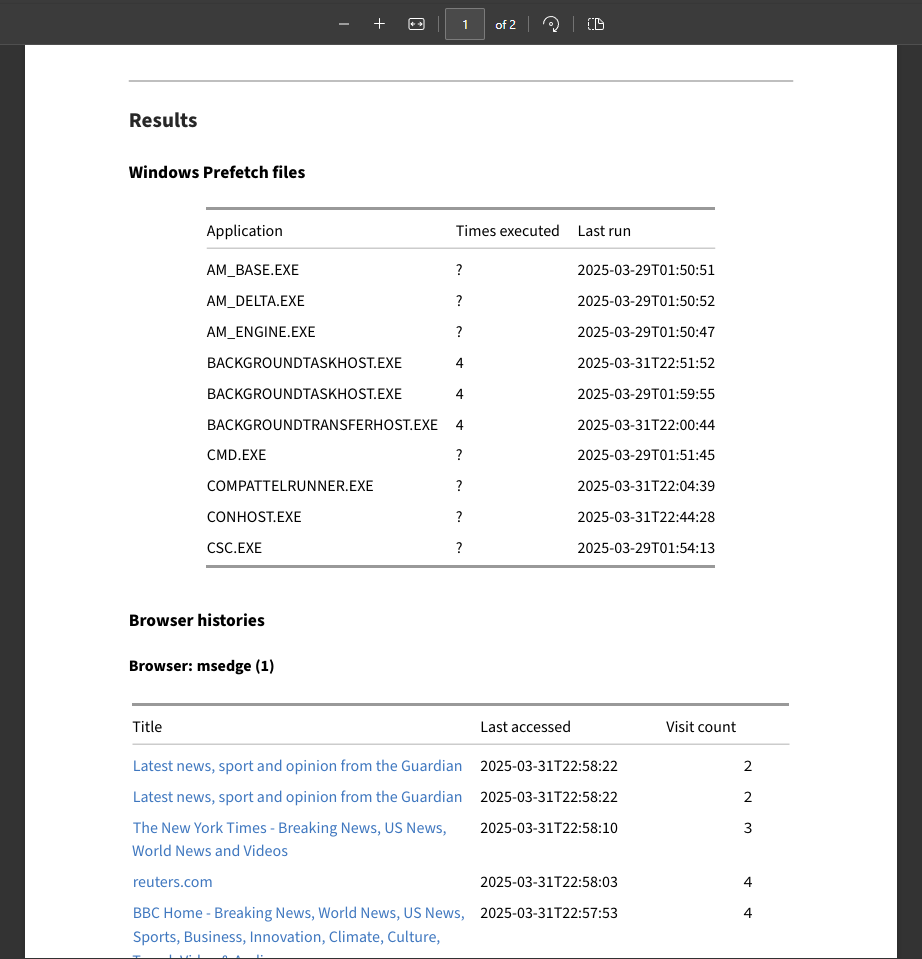
\includegraphics[width=1\linewidth]{human-reporting.png}
\caption{Sample PDF report generated by AKF
renderers}\label{fig:scenario-report}
\end{figure}

Of course, other options exist for generating human-readable (and
machine-readable) reporting from an AKF-generated dataset. For example,
the analysis features provided by tools such as Plaso
\cite{Log2timelinePlaso2025} and those developed by Eric Zimmerman
\cite{zimmermanEricZimmermansTools} can be used to supplement the
existing reporting and validation features of AKF. These tools can be
directly integrated into AKF workflows in the future, although this is
not currently the case.

After generating the scenario itself and any metadata and reporting that
should be included with the dataset, the challenge of distributing this
information remains. More precisely, how do we make our dataset as
accessible, reusable, and discoverable as possible?

\section{Distribution and community
reproducibility}\label{distribution-and-community-reproducibility}

A key challenge identified by Grajeda et al.~was the difficulty in
reproducing results in the field of digital forensics. While this is
primarily attributed to the \emph{availability} of forensic datasets in
general, it can also be attributed to challenges in the
\emph{reproducibility} of creating synthetic datasets.

Before addressing the low-level use of AKF as part of \autoref{chapter-six}, we briefly discuss the infrastructure needed to
support community usage of the outputs of AKF scenarios and synthetic
datasets as a whole. Note that for the remainder of this section,
scenarios and datasets are both implied to be synthetic, as the
principles of reproducibility are less applicable to real-world
datasets.

There are four elements that must be distributed with a scenario to make
a dataset (and its results) reproducible:

\begin{itemize}
\tightlist
\item
  Any core outputs or individual artifacts generated from the virtual
  machine.
\item
  Any metadata, ground truth, or other reporting that describes the
  scenario.
\item
  The OS-specific ``base image'' used to create the dataset, typically a
  virtual machine with a newly installed operating system on which all
  synthesizer actions are performed.
\item
  The precise instructions required to build the scenario from the
  provided base image, whether human- or machine-readable instructions.
\end{itemize}

Forensic datasets have long included core outputs and individual
artifacts well before the development of AKF and other synthesizers;
there is limited value in a forensic scenario without anything to
analyze. Various forms of ground truth have also long been a part of
forensic datasets in multiple forms; some educational datasets include
PDF answer keys, while some research datasets have been labeled in a
structured format to include metadata about the dataset.

However, less common are detailed instructions to build the overall
scenario. Manually constructed datasets rarely describe the actions
taken to create a scenario in detail; for example, the educational
M57-Patents scenario built by Woods et al.
\cite{woodsCreatingRealisticCorpora2011} provides an instructor PDF
with a high-level timeline of actions taken in English. This detail is
sufficient for educational purposes but is too imprecise to guarantee
that others following this timeline will construct the image in the same
manner as intended. As described in \autoref{challenges-in-developing-synthetic-datasets}, non-determinism can be
acceptable and even desirable in educational contexts but is less
desirable for tool validation and research.

Even rarer in manually constructed datasets is the inclusion of a base
image representing the machine's state before any actions are performed.
This may be attributable to both copyright concerns and a perception
that knowledge of the operating system alone is sufficient to rebuild
the base image; while it is true that setting up a virtual machine is
straightforward, any need for human interpretation introduces a source
of non-determinism that could be eliminated.

Synthesizers significantly improve on the lack of precise instructions;
their machine-readable scripts both document and execute the exact
instructions needed to reconstruct a scenario. However, this depends on
the availability of an OS- and synthesizer-specific base image; many
synthesizers expect their users to follow a set of human-readable
instructions to prepare a virtual machine specifically for use with that
synthesizer.

Where copyright issues are not a concern, synthetic images should aim to
include a complete definition of a virtual machine to be used as the
base image. A base image may be a full, hypervisor-specific virtual
machine (archiving and compressing the entirety of the associated
virtual machine folder), a hypervisor-independent virtual appliance (in
a format such as OVF), or another infrastructure-as-code solution to
define and build virtual machines, such as Vagrant.

AKF is designed to provide all four of these elements in every scenario
it creates; elements 1, 2, and 4 are inherent to all synthesizers, while
base images can be provided as Vagrantfiles as described in \autoref{setup-and-basic-usage}. This ensures that
results from AKF-generated scenarios are reproducible from both a
dataset creation and dataset usage perspective.

Although not explored as part of this thesis, the inclusion of all four
of these elements as part of a well-structured, standardized
distribution format could be used to build a distribution platform
similar to CFReDS but with more powerful discovery and querying
functionality. While the contents of the scenario are primarily
described by CASE, it may also be possible to perform queries based on
the contents of Vagrantfiles and AKF scripts. For example, a user may
want to search for all images that use the agent-based Chromium artifact
generation described in \autoref{akf-implementation}, which can be achieved by searching for the inclusion of
the relevant AKF libraries in the scenario's scripts. However, this does
not address the challenge of storing and distributing scenarios
efficiently to support such a platform; this is discussed in
\autoref{distribution}.

With the reproducibility and value of AKF-generated scenarios
established, we now discuss how to invoke and leverage the underlying
technologies that provide these benefits.

\chapter{Building scenarios}\label{chapter-six}

This chapter addresses the modules responsible for allowing users to
invoke the framework through a standard Python script and a high-level
YAML file. It also addresses the generative AI modules that can assist a
user in building a scenario. These modules are depicted in
\autoref{fig:scenarios-simple} below, with a more detailed diagram
located in \autoref{appendix-a} as
\autoref{fig:architecture-full-a}.

\begin{figure}[h]
\centering
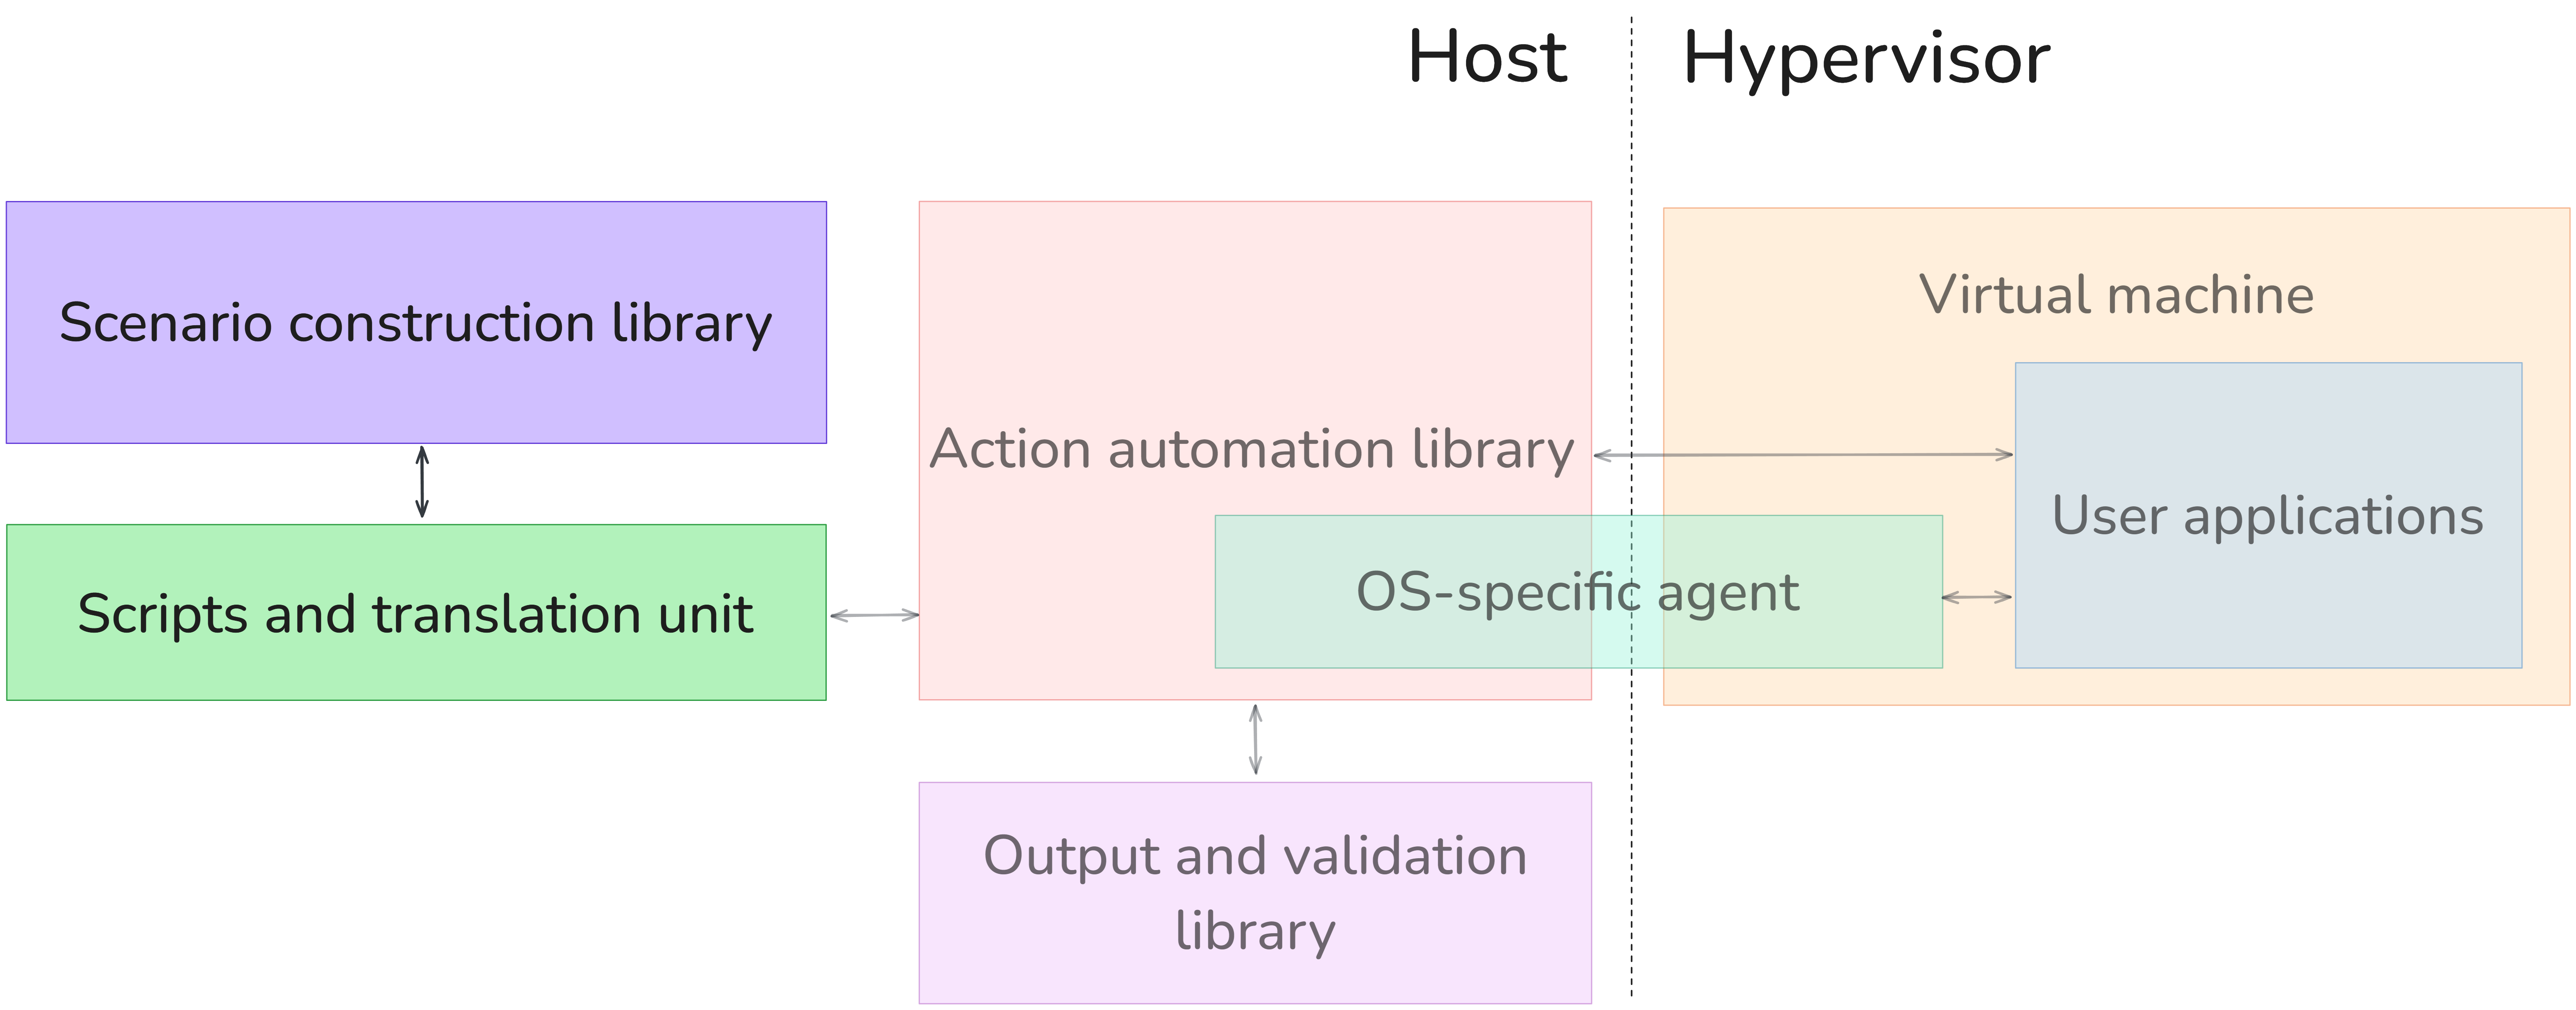
\includegraphics[width=1\linewidth]{scenarios-simple.png}
\caption{Simplified AKF architecture diagram for scenario construction
modules}\label{fig:scenarios-simple}
\end{figure}

At this point, we have provided the functionality for automating
artifact generation in a near-deterministic manner with comprehensive
logging and reporting. However, there is still the challenge of exposing
this functionality in a user-friendly manner. At a high level, there are
two primary ways to define an input to a synthesizer. These formats
describe the process (the \emph{how}) of placing artifacts and
performing actions:

\begin{itemize}
\tightlist
\item
  An \textbf{imperative} format, in which the synthesizer is provided
  instructions in an imperative programming language, and the developer
  must provide the exact instructions for the synthesizer to take
  through some exposed API.
\item
  A \textbf{declarative} format, in which the synthesizer is provided a
  file that describes the desired elements of the result, and it is up
  to the synthesizer to execute the instructions necessary to achieve
  the result.
\end{itemize}

However, the challenge of deciding \emph{what} actions to perform
remains. It is still mainly the responsibility of instructors to provide
background noise and other realistic artifacts to insert into a
scenario. Additionally, although synthesizers make it easier to place
files at desired locations or visit websites, these scenario elements
must be defined and created beforehand. More precisely, these represent
challenges in two specific areas:

\begin{itemize}
\tightlist
\item
  \textbf{Generating standalone artifacts}: Users must include email
  conversations, documents, and other application-specific artifacts to
  be generated as part of a scenario.
\item
  \textbf{Creating the scenario itself}: Users must combine these
  standalone artifacts to generate a cohesive scenario, following a
  theme such as corporate espionage or ransomware attacks.
\end{itemize}

This chapter addresses the challenges of providing APIs for complex
GUI-driven applications and creating background noise. More precisely,
we address two questions -- how do we invoke AKF's automation systems,
and how does AKF assist a user in building a scenario? Here, we explore
AKF's imperative and declarative syntaxes and the viability of using
generative AI to assist in building individual files and complete
scenario descriptions.

\section{Scripting background}\label{scripting-background}

We begin by analyzing how synthesizers accept instructions for execution
-- more precisely, how do users define the sequence of operations that
the synthesizer should take to create the dataset?

For many of the frameworks created in the last decade, users define
scenarios by using a Python library to interact with the framework. The
library is responsible for setting up the virtualized environment and
performing high-level actions on the environment, abstracting away the
underlying calls to the hypervisor from the scenario developer. This
code-based approach represents an \emph{imperative} strategy for
scenario creation, where the user describes how the dataset should be
created by defining the exact order and means to perform synthesizer
actions. It is worth noting that the language used to interact with the
synthesizer's API does not need to match the language used to implement
the synthesizer itself, although this is often the case. For example,
the automation framework Playwright is implemented in TypeScript,
initially exposing a Node.JS API
\cite{MicrosoftPlaywrightpython2025}; today, Playwright provides
APIs in Python, Java, and C\#.

In contrast, custom scenario formats provided by D-FET
\cite{williamCloudbasedDigitalForensics2011}, SFX
\cite{russellForensicImageDescription2012}, and Yannikos et al.
\cite{yannikosDataCorporaDigital2014} follow a different approach.
For these synthesizers, a custom high-level language describes the
desired final state of the dataset. Instead of importing libraries and
writing code, users state the desired elements of the forensic dataset,
allowing the synthesizer to decide how to create the desired dataset --
a \emph{declarative} strategy for scenario creation. The specifics of
state management and execution are delegated to the synthesizer.

Consider the following declarative SFX code taken from Russell et
al.~shown in \autoref{lst:6.1a}
\cite{russellForensicImageDescription2012}:

\begin{lstlisting}[label={lst:6.1a}, caption={Declarative SFX scenario with web browsing \cite{russellForensicImageDescription2012}}, language=XML]
<disk>
    <partition index="p1" hidden="0" size="48M" type="ntfs">
        <base os="windows7x64"/>
        <user username = "Gordon">
             <browserhistory browser="firefox">
                 <url link="bbc.co.uk" time="13:14:00 1 Jan 2013"/>
             </browserhistory>
        </user>
    </partition>
</disk>
\end{lstlisting}

Here, a Windows 7 partition is created as part of a larger disk image.
The partition is loaded in a virtual machine to create a user called
``Gordon,'' who uses Firefox to browse the internet. (This simple web
browsing scenario will be reused throughout this chapter to demonstrate
several code examples.)

The same might be expressed in ForTrace
\cite{gobelForTraceHolisticForensic2022} as shown in
\autoref{lst:6.1b}, excluding additional code required for ground truth
and disk image generation:

\begin{lstlisting}[label={lst:6.1b}, caption={Imperative ForTrace scenario with web browsing \cite{gobelForTraceHolisticForensic2022}}, language=Python]
from fortrace.core.vmm import Vmm
from fortrace.utility.logger_helper import create_logger
from fortrace.core.vmm import GuestListener

if __name__ == "__main__":
    logger = create_logger('fortraceManager', logging.DEBUG)
    macsInUse = []
    guests = []
    
    guestListener = GuestListener(guests, logger)
    virtual_machine_monitor1 = Vmm(macsInUse, guests, logger)
    # boottime expressed as "%Y-%m-%d %H:%M:%S"
    guest = virtual_machine_monitor1.create_guest(guest_name="w-guest01", platform="windows", boottime="2013-01-01 13:14:00")

    browser_obj = guest.application("webBrowserFirefox", {'webBrowser': "firefox"})
    browser_obj.open(url="bbc.co.uk")
    while browser_obj.is_busy:
        time.sleep(2)
    browser_obj.close()
\end{lstlisting}

Although these two code blocks have the same expressive power (that is,
they achieve the same overall outcomes), there is a clear difference in
the complexity and length between them. It is significantly easier to
read and write the declarative XML in the first code block, as it
abstracts away the need to instantiate various synthesizer objects and
call specific methods. By extension, this also allows for a common
declarative syntax to be used across multiple synthesizers since
low-level synthesizer details do not need to be exposed as part of the
declarative syntax.

The primary benefit of an imperative approach to generation is its
flexibility; on a Python-based synthesizer, one can simply import
another library to extend the functionality of the base scenario
definition. This flexibility naturally comes at the expense of a greater
learning curve. Although many digital forensic specialists are likely to
have programming experience, it is far easier to learn a restricted
declarative specification (like XML) than an entire programming
language, which may entail additional setup (such as installing an IDE,
dependencies, and so on).

When accessibility is preferred over functionality, declarative syntaxes
can be more valuable than imperative syntaxes. Some scenario developers,
such as classroom instructors, may not need the low-level control
provided by an imperative syntax or a complete programming language such
as Python. It also takes time to learn about the functionality exposed
by the synthesizer's library, not to mention learning the programming
language itself. These are the primary motivators behind supporting
well-defined declarative syntaxes.

Of course, low-level control is still important, especially when
external libraries must be used to implement functionality not
inherently exposed by a synthesizer. For this reason, some synthesizers
support both declarative and imperative scripts to generate scenarios.
For example, the Python-based hystck and ForTrace frameworks
\cite{gobelNovelApproachGenerating2020,gobelForTraceHolisticForensic2022}
allow users to write YAML scripts to execute actions. Support for both
formats can be implemented through various means, such as
declarative-to-imperative translators. (While not explored in this
thesis, it is also worth noting the GUI-based interfaces provided by
Yannikos et al. \cite{yannikosDataCorporaDigital2014} and ForGe
\cite{vistiAutomaticCreationComputer2015} for building scenarios.)

AKF supports an imperative syntax (through its Python API) and a custom
declarative syntax. Unlike prior synthesizers, AKF's declarative syntax
supports both execution and declarative-to-imperative translation,
allowing users to quickly create and modify imperative scripts from
high-level declarative descriptions.

\section{Setup and basic usage}\label{setup-and-basic-usage}

Like many of its predecessors, AKF implements its functionality and
exposes its API in the same language, Python 3. There are numerous
advantages to a Python-based API; besides the relatively low difficulty
of setting up and using Python, its rich ecosystem allows scenarios to
be extended through other libraries from the Python ecosystem. For
example, if a user wanted to conditionally execute certain parts of a
scenario by testing if a particular remote service is currently online,
a user could use the Requests library \cite{Requests31Documentation}
to issue an HTTP request out-of-band before performing the same action
in a virtualized environment.

Users must install two foundational technologies for AKF to operate --
Python 3.11 (or later) and a supported hypervisor. AKF currently only
supports VirtualBox as its hypervisor, though QEMU/libvirt has also been
used in prior synthesizers. AKF uses
\passthrough{\lstinline!pyproject.toml!} to define Python library
dependencies, which can be installed into a virtual environment using a
package manager such as \passthrough{\lstinline!pip!} or
\passthrough{\lstinline!uv!}.

At this point, a virtual machine must be prepared for use with AKF. As
with prior synthesizers, it is possible to manually configure a machine
by downloading a supported operating system and creating a new virtual
machine from scratch. The manual process, which is similar to that of
other synthesizers, is as follows:

\begin{itemize}
\tightlist
\item
  Download an ISO or pre-prepared virtual machine from a distributor
  with the desired operating system.
\item
  If necessary, install the operating system on a new virtual machine.
\item
  Configure the virtual machine with the desired host resources,
  including two network interfaces -- one connected to the NAT adapter
  for general internet usage and one connected to the host-only adapter
  for agent communications.
\item
  Create an administrative user with known credentials. Configure the
  operating system as desired to reduce friction with the synthesizer
  (such as disabling UAC prompts, enabling auto-logon, and so on.)
\item
  Build and copy the OS-specific AKF agent to the virtual machine,
  configuring it as a startup application. Add firewall rules to ensure
  that the host and agent are able to communicate.
\end{itemize}

After this process, the virtual machine can be cloned and reused in
multiple AKF scenarios. Although relatively straightforward, this
process is still time-consuming, especially when adapting this process
to new operating systems. While a prepared AKF virtual machine can
theoretically be distributed (in a virtual appliance format such as
OVF), this can run into legal issues if the software on the underlying
operating system is copyrighted.

As a result, AKF uses modern infrastructure-as-code solutions to vastly
simplify the setup of new virtual machines. Vagrant, developed by
HashiCorp, is a tool for rapidly building development environments
\cite{HashicorpVagrant2025}. It allows users to define and build
virtual machines on several virtualization platforms, including
VirtualBox and VMWare. Virtual machines are built by configuring a base
image according to a Vagrantfile, which describes hypervisor-specific
configuration options and instructions to configure the machine. The
Vagrantfile can be distributed to users, allowing them to build the same
virtual machine without distributing virtual drives. (A similar approach
of distributing the ``differences'' of base images is used to reduce the
size of distributed forensic datasets by EviPlant
\cite{scanlonEviPlantEfficientDigital2017}, as described in
\autoref{distribution}.)

The AKF Windows agent includes a Vagrantfile for creating a new Windows
11 virtual machine with the agent installed and configured, which can
easily be adapted for other platforms and hypervisors. The
Vagrantfile(s) used to generate a dataset should be included with the
dataset itself to maximize reproducibility, as described in \autoref{distribution-and-community-reproducibility}. A robust ecosystem of Vagrant boxes for varying Linux
distributions and Windows versions exists, many of which can be pulled
from the Vagrant public registry
\cite{hashicorpHashiCorpCloudPlatform}. When combined with the
flexibility of Vagrant over multiple virtualization platforms, this can
significantly improve the reproducibility and usability of AKF across
many platforms. It should also be noted that Vagrant can configure and
build larger environments with multiple machines. For organizations that
can express corporate environments as Vagrantfiles, AKF could perform
artifact generation at scale, allowing for incident response scenarios
reflecting real-world networks and events.

Following setup, developers can build scenarios using the AKF core
libraries (\passthrough{\lstinline!akflib!}) and the API of the
platform-specific agent installed onto the virtual machine. This
reflects typical imperative usage, in which environment setup, artifact
generation, and output generation are handled explicitly through a
script executed through the Python interpreter.

A simple AKF script achieving the same outcomes as the ForTrace and SFX
scripts above is shown in \autoref{lst:6.2a}:

\begin{lstlisting}[label={lst:6.2a}, caption={Example of an imperative AKF scenario}, language=Python]
from akf_windows.api.chromium import ChromiumServiceAPI
from akflib.core.hypervisor.vbox import VBoxExportFormatEnum
from akflib.core.hypervisor.vbox import VBoxHypervisor
from pathlib import Path

# Instantiate a hypervisor object tied to a specific virtual machine
vbox_obj = VBoxHypervisor("akf-windows-1")

# Start the virtual machine
vbox_obj.start_vm(wait_for_guest_additions=True)

# Visit a single website
with ChromiumServiceAPI.auto_connect(vbox_obj.get_maintenance_ip()) as chromium_service:
    chromium_service.kill_edge()
    chromium_service.set_browser("msedge")
    page = chromium_service.browser.new_page()
    page.goto("bbc.co.uk")  

# Stop the virtual machine
vbox_obj.stop_vm(force=False)

# Export the virtual machine to a disk image
vbox_obj.create_disk_image(
    Path("C:/Users/kisun/Desktop/akf-windows_1.raw"),
    VBoxExportFormatEnum.RAW
)
\end{lstlisting}

Here, we create a new \passthrough{\lstinline!VBoxHypervisor!} instance
that will allow us to start and interact with a VirtualBox machine
called \passthrough{\lstinline!akf-windows-1!} (created previously with
Vagrant as described above). To initialize the Chromium subservice, we
query VirtualBox for the IP address of the host-only adapter, then use
the \passthrough{\lstinline!auto\_connect!} convenience method to
automatically perform the required RPyC setup and return an instance of
\passthrough{\lstinline!ChromiumServiceAPI!}. This instantiated API
allows us to interact with Microsoft Edge on the virtual machine over
RPyC (which is abstracted away from the user); as part of the context
manager, the RPyC connection is automatically closed at the end of the
\passthrough{\lstinline!with!} block. Finally, we create a raw disk
image and save it to the desktop.

With this in mind, how do we expose this same functionality through a
declarative syntax?

\section{Declarative usage}\label{declarative-usage}

As described previously, declarative inputs are well-structured files
with a fixed set of available actions -- effectively forming an API --
where each entry in the file specifies an action or artifact to be
generated as part of a dataset. Individual entries may contain
additional configuration data that modifies how that specific action or
artifact is generated. An \emph{interpreter} is responsible for parsing
and acting on the entries in the declarative file.

Interpreters can act on declarative formats in one of two ways. The
first is \emph{execution}, in which the elements of the declarative
script are directly interpreted to generate imperative API calls. This
is characteristic of synthesizers that only support declarative script
inputs, exposing no low-level APIs. Execution takes advantage of the
high-level nature of declarative scripts; a declarative script can
remain the same even if the libraries that execute it change, so long as
the interpreter is updated accordingly. The second is
\emph{translation}, in which the declarative script is used to generate
an equivalent imperative script adhering to a particular synthesizer's
API. This allows the declarative script to be used as a ``base'' for
creating imperative scripts, such that an experienced scenario developer
can modify the generated imperative script as needed. Imperative scripts
can be regenerated from the same declarative script to reflect updates
in library usage so long as the interpreter is updated accordingly,
inheriting the evergreen nature of declarative scripts.

It is important to note that a declarative syntax, which may be more
``rigid'' in structure, does not preclude the use of non-determinism or
randomness. One notable example of this is the discrete-time Markov
chains used by Yannikos et al.~to express scenarios in a probabilistic
manner, with each state of the Markov chain representing a particular
action taken by the synthesizer (such as sending an email or deleting a
file) \cite{yannikosDataCorporaDigital2014}. These chains are
evaluated at runtime to generate multiple unique datasets from a single
description.

The challenges of defining a suitable declarative syntax for a
particular synthesizer are not unlike the challenges faced in general
programming language design. There are several key factors to the
success of imperative programming languages that extend to declarative
syntaxes, some of which are derived from Finkel and described as follows
\cite{finkel1996advanced}:

\begin{itemize}
\tightlist
\item
  The language should be \textbf{simple}, using as few basic concepts as
  possible. This makes code easier to read and write, an important
  aspect for users with limited programming experience.
\item
  The language should be \textbf{modular}, such that the role and
  interfaces of individual program units are clear.
\item
  The language should be \textbf{predictable}, such that users can apply
  their existing knowledge of a synthesizer to quickly implement or add
  new features to a scenario.
\item
  The language should \textbf{abstract} as much as possible away from
  the user, such that the minimum information needed to fulfill artifact
  generation is exposed to the user.
\end{itemize}

The most important factor, however, is an awareness of the
\textbf{purpose} of the declarative syntax. The purpose of a synthesizer
is to make it easier to generate forensic artifacts and datasets. The
declarative language should reflect this, focusing on making actions and
artifacts as easy to declare and customize as possible. (These five
factors are particularly important in allowing LLMs to reliably generate
declarative scenarios, as described in \autoref{using-llms-for-high-level-scenarios}.)

In designing the AKF declarative syntax, the declarative syntaxes of
prior synthesizers and unrelated technologies were evaluated. An
analysis of some of these syntaxes, with examples, is described briefly
in \autoref{historical-declarative-syntaxes}.
However, the two syntaxes that contributed most to the AKF declarative
syntax were those of ForTrace and Ansible, described in the following
section.

\subsection{Existing declarative
syntaxes}\label{existing-declarative-syntaxes}

ForTrace \cite{gobelForTraceHolisticForensic2022} uses YAML to
express scenarios in a declarative manner. ForTrace significantly
influenced both the AKF declarative syntax itself and the implementation
of the declarative interpreter, primarily because it was the sole
open-source synthesizer with both imperative and declarative support.
\autoref{lst:6.3.1a} demonstrates a simple example of a ForTrace
declarative scenario:

\begin{lstlisting}[label={lst:6.3.1a}, caption={Declarative ForTrace scenario with web browsing \cite{gobelForTraceHolisticForensic2022}}, ]
name: haystack-example
description: A example action suite to generate a haystack (traffic)
author: MPSE Group
seed: 1234
collections:
  c-http-0:
    type: http
    urls: ./generator/friendly_urls.txt
settings:
  host_nfs_path:
  guest_nfs_path:
applications:
hay:
  h-http-0:
    application: http
    amount: 3
    collection: c-http-0
needles:
  n-http-0:
    application: http
    url: dasec.h-da.de
    amount: 1
dumps:
  d-dump-0:
    dump-type: mem
    dump-path: /home/fortrace/gendump.file
\end{lstlisting}

At a high level, ForTrace scenarios contain five distinct elements:

\begin{itemize}
\tightlist
\item
  Metadata about the scenario, such as the scenario's name, description,
  and author.
\item
  ``Collections'' of data that can be reused throughout the scenario in
  supported application types, such as a newline-separated list of URLs.
\item
  Configuration options that may be applied to all actions of a
  particular action type or the entire scenario.
\item
  The actual artifacts to create as part of the
  \passthrough{\lstinline!hay!} and \passthrough{\lstinline!needles!}
  sections, where \passthrough{\lstinline!hay!} includes artifacts that
  should be considered background noise, and
  \passthrough{\lstinline!needles!} includes artifacts that should be
  considered significant. Each artifact contains a unique ID, an
  application type (the \passthrough{\lstinline!application!} key), and
  arguments specific to the application responsible for generating the
  artifact, such as the URLs for web browsing.
\item
  Any core outputs that should be created as part of the scenario.
\end{itemize}

This file is passed into a ``generator,'' which parses the contents of
the YAML file to prepare various internal data structures, initialize
the virtual machine, and then execute the actions specified in the
\passthrough{\lstinline!hay!} and \passthrough{\lstinline!needles!}
sections in a random order according to the
\passthrough{\lstinline!seed!} key. Depending on the value of the
\passthrough{\lstinline!application!} key, the data for that action is
passed to an application-specific handler that interacts with the
running virtual machine using existing ForTrace libraries. Once all the
actions have been executed, the generator creates any requested outputs
(such as volatile memory dumps) and shuts down the virtual machine.

This analysis provided insight into the design decisions and
functionality required to execute actions from the high-level
descriptions of a scenario. In particular, it demonstrates the need for
actions or artifacts to be defined consistently and flexibly so that
program state and other data can be passed to application-specific
libraries as needed. It also demonstrates the need for various levels of
configuration, including scenario-wide configuration,
application-specific configuration, and action/artifact-specific
configuration. ForTrace implements these features in a somewhat awkward
manner; in fact, nearly all declarative language support is contained in
a single file, with a hardcoded ``router'' handling each unique
\passthrough{\lstinline!application!} type. This makes it difficult to
add support for new applications without significant effort,
particularly because the generator must be aware of every possible
action/artifact type ahead of time.

With these priorities and issues from ForTrace identified, are there
ideas from other technologies that can be used to address them? That is,
are there other technologies designed to execute a large set of complex
actions using a simple but flexible and configurable syntax, and how
does it work? Ansible, the second major inspiration for the AKF
declarative syntax, precisely addresses these questions.

Ansible \cite{AnsibleAnsible2025} is an open-source automation
framework often used to remotely configure Windows and Linux machines at
scale, allowing organizations to manage many machines at once without
installing orchestration software on these machines in advance. To
achieve this, users write \emph{playbooks}, which are simple YAML files
that contain one or more \emph{plays}. Each play is simply a set of
\emph{tasks} run on multiple machines simultaneously, and each task
depends on a \emph{module} designed to achieve a single, specific
outcome.

An example of an Ansible playbook can be seen in \autoref{lst:6.3.1b},
which contains a single play to configure an Apache webserver.

\begin{lstlisting}[label={lst:6.3.1b}, caption={Minimal Ansible playbook for updating an Apache server \cite{ansibleprojectcontributorsAnsiblePlaybooks}}, ]

- name: Update web servers
  hosts: webservers
  remote_user: root
  tasks:
  - name: Ensure apache is at the latest version
    ansible.builtin.yum:
      name: httpd
      state: latest
  - name: Write the apache config file
    ansible.builtin.template:
      src: /srv/httpd.j2
      dest: /etc/httpd.conf
\end{lstlisting}

This play uses the \passthrough{\lstinline!yum!} package manager to
install Apache before copying a local configuration file to the remote
host. \passthrough{\lstinline!ansible.builtin.yum!} and
\passthrough{\lstinline!ansible.builtin.template!} are both modules,
which accept parameters passed as a YAML dictionary. These modules are
part of the \passthrough{\lstinline!ansible.builtin!} collection
included with all default Ansible installations.

Although Ansible contains many features that contribute to its
flexibility, the two important concepts relevant to AKF are \emph{roles}
and \emph{modules}. Roles are a collection of Ansible resources that
typically achieve some ``larger'' reproducible goal, typically by
running multiple tasks and leveraging variables, configuration options,
and files included as part of the role. Roles can include
\emph{modules}, which are standalone imperative scripts (typically in
Python) that accept arguments, execute code based on those arguments,
and return data using well-structured interfaces. As shown above, these
modules can be called and executed from playbooks; they can also be
executed independently on the command line.

These concepts are highly relevant to synthesizers, which must support
application-specific actions and group these actions together in a
flexible, well-defined manner. As described in \autoref{the-akf-agent}, each RPyC subservice of an AKF agent
exposes a group of application-specific automation methods. The
functionality of each of these groups must be re-exposed in a
declarative manner, which can be achieved by adapting the concept of
Ansible roles and modules to AKF.

Together, the ForTrace and Ansible syntaxes provide three concepts that
are reflected in the AKF syntax, described further in the following
section:

\begin{itemize}
\tightlist
\item
  The overall structure and contents of the declarative YAML file.
\item
  An action syntax that allows us to declare individual actions,
  referring to those actions by name, and pass arguments directly to
  that action for \emph{translation} or \emph{execution}.
\item
  A modular architecture that allows us to define the supported
  arguments of each action and expose them to the declarative
  interpreter while also being decoupled from the standard imperative
  library as much as possible.
\end{itemize}

\subsection{The AKF declarative
syntax}\label{the-akf-declarative-syntax}

The AKF declarative syntax is very similar to the Ansible playbook
syntax. Declarative scripts are comprised of metadata, global
configuration, libraries to import, and individual tasks to execute as
part of the scenario. Each task refers to a single \emph{module} by name
using a qualified Python import path, accepting a dictionary of
arguments in addition to global configuration overrides.

Like Ansible, individual modules are implemented as well-defined
subclasses of \passthrough{\lstinline!AKFModule!}, an abstract base
class that serves as the root of all AKF declarative modules. Each
module must define Pydantic models that specify the arguments accepted
by the module. The arguments declared in the YAML file are then passed
to these module-specific Pydantic models for validation, after which the
\passthrough{\lstinline!AKFModule!} must perform one of two tasks:

\begin{itemize}
\tightlist
\item
  \textbf{Execution}: When instructed to perform actions directly from
  the declarative script, the \passthrough{\lstinline!AKFModule!} should
  import AKF core libraries and agent APIs to perform the required
  actions.
\item
  \textbf{Translation}: When instructed to translate the declarative
  script, the \passthrough{\lstinline!AKFModule!} should generate the
  equivalent code that \emph{would} perform the required actions if
  executed through a standard Python interpreter with the necessary
  libraries installed.
\end{itemize}

The ability of AKF to both execute and translate declarative scripts
provides significant flexibility to scenario developers. To the best of
our knowledge, prior synthesizers have only supported direct execution
from declarative scripts, which limits the opportunities to use
declarative scripts as a ``starting point'' for writing more complex
imperative scripts. (In fact, the code in \autoref{lst:6.2a} was
primarily derived from the auto-generated code shown in
\autoref{lst:6.3.2a}.)

An example of a minimal AKF scenario, carrying out the same actions as
the SFX, ForTrace, and imperative AKF script above, can be seen in
\autoref{lst:6.3.2a}:

\begin{lstlisting}[label={lst:6.3.2a}, caption={Example of a declarative AKF scenario}, ]
name: Minimal scenario
description: Browses to the BBC website and exports a disk image.
author: Lloyd Gonzales
seed: "0"
libraries:
  - akflib.modules
  - akf_windows.modules
actions:
  - name: Instantiate a hypervisor object tied to a specific virtual machine
    module: vbox_start
    args:
      machine_name: "akf-windows-1"
  - name: Start the virtual machine
    module: vbox_start_machine

  # Visit a website using Microsoft Edge. A temporary instance of the Chromium
  # subservice API is created for the lifetime of this module.
  - name: Visit a single website
    module: chromium_visit_urls
    args:
      browser: "msedge"
      urls: 
       - "bbc.co.uk"

  # Stop the virtual machine and export the virtual machine to a disk image.
  - name: Stop the virtual machine
    module: vbox_stop_machine
    args:
      force: false
  - name: Export the virtual machine to a disk image
    module: vbox_create_disk_image
    args:
      output_path: "C:/Users/user/Desktop/akf-windows_1.raw"
      image_format: "raw"
\end{lstlisting}

The \passthrough{\lstinline!akf-translate!} interpreter, which is added
to PATH when installing \passthrough{\lstinline!akflib!}, handles both
execution and translation from a declarative script. It uses the same
underlying library calls as the imperative code in \autoref{lst:6.2a}.
To use this declarative script with
\passthrough{\lstinline!akf-translate!}, one of the following commands
in \autoref{lst:6.3.2b} can be used:

\begin{lstlisting}[label={lst:6.3.2b}, caption={Sample usage of the akf-translate utility}, language=sh]
# Translate this scenario to a valid Python script and save it to disk
akf-translate scenarios/thesis.yaml --translate --output-file scenarios/thesis.py

# Execute this scenario directly
akf-translate scenarios/thesis.yaml --execute
\end{lstlisting}

AKF declarative scripts, which are simply large YAML dictionaries,
contain three distinct elements. The first is a set of high-level
metadata keys associated with the scenario. The second is a set of
scenario-wide configurations; in particular, it lists the libraries
containing the necessary modules to execute or translate this imperative
script. Finally, scripts list a sequence of actions, typically a
\passthrough{\lstinline!module!} specified by name and a dictionary of
\passthrough{\lstinline!args!}.

The execution flow of \passthrough{\lstinline!akf-translate!} itself is
straightforward. Given a path to a YAML script, the interpreter will
load the necessary libraries and configuration keys defined in the file
and instantiate resources accordingly. This may include setting aliases
for module names, verifying that all required modules are available,
setting the \passthrough{\lstinline!random!} seed, and so on. Then, the
interpreter runs each module under the \passthrough{\lstinline!actions!}
key with the provided arguments and configuration in order, continuing
until all actions have been processed.

Modules can read and modify a global state dictionary that allows
otherwise independent modules to cooperate. For example, suppose that a
module creates a new context manager in a \passthrough{\lstinline!with!}
block, causing the indentation level of the translated code to increase.
Successive modules can read the state dictionary to retrieve context
variables and correctly indent generated code. Additionally, this allows
for ``outputs,'' such as CASE bundles, to be passed and gradually
constructed across modules. This design allows for context-aware code
generation and action execution.

Modules are located and executed using Python's dynamic import system.
These modules can be located in any library so long as they can be found
through Python's import system. For example, both
\passthrough{\lstinline!akflib!} and the AKF Windows agent contain their
own declarative module libraries, leveraging functionality specific to
each code repository. All modules in the script are located and
``cached'' at the start of script execution, which allows for
verification and runtime efficiency.

This design allows declarative modules to be written independently of
the libraries they depend on, reducing the ``impact'' of supporting
declarative features on the core imperative libraries. In fact, this
independence allows for the AKF module system to be used in
general-purpose scripting, similar to Ansible; it is not tightly bound
to the creation of forensic scenarios and artifacts. That said, the
existing declarative modules of AKF expose nearly all existing
functionality provided by \passthrough{\lstinline!akflib!}, including
PDF report generation, virtual machine interaction, and more.

The list of declarative modules available through
\passthrough{\lstinline!akflib!} and the Windows agent is described in
\autoref{tbl:akf-declarative-modules} below. Note that these modules are
referred to by their alias, not their fully-qualified module paths.


{
\small % 10pt font
\setstretch{1} % Single spacing
\begin{longtable}[]{@{}
  >{\raggedright\arraybackslash}p{(\linewidth - 2\tabcolsep) * \real{0.3}}
  >{\raggedright\arraybackslash}p{(\linewidth - 2\tabcolsep) * \real{0.7}}
@{}}
\caption{Available AKF declarative modules}\label{tbl:akf-declarative-modules} \\
\toprule\noalign{}
\begin{minipage}[b]{\linewidth}\raggedright
Name
\end{minipage} & \begin{minipage}[b]{\linewidth}\raggedright
Description
\end{minipage} \\
\midrule\noalign{}
\endhead
\bottomrule\noalign{}
\endlastfoot
\passthrough{\lstinline!create\_akf\_bundle!} & Creates a new CASE
bundle for use throughout the declarative scenario. \\
\passthrough{\lstinline!write\_akf\_bundle!} & Write the contents of the
currently active CASE bundle to disk as a JSON-LD file. \\
\passthrough{\lstinline!render\_akf\_bundle!} & Pass the currently
active CASE bundle through a set of provided renderers and construct a
valid PDF using Pandoc. \\
\passthrough{\lstinline!vbox\_start!} & Create a new VirtualBox instance
bound to a specific virtual machine by name. \\
\passthrough{\lstinline!vbox\_start\_machine!} & Power on the currently
active virtual machine. \\
\passthrough{\lstinline!vbox\_stop\_machine!} & Power off the currently
active virtual machine. \\
\passthrough{\lstinline!vbox\_create\_disk\_image!} & Export a disk
image of the current virtual machine. \\
\passthrough{\lstinline!artifact\_service\_start!} & Remotely start and
connect to the subservice responsible for collecting Windows
artifacts. \\
\passthrough{\lstinline!artifact\_service\_stop!} & Disconnect from the
subservice responsible for collecting Windows artifacts. \\
\passthrough{\lstinline!prefetch!} & Analyze all prefetch files on disk
and construct their corresponding CASE objects. \\
\passthrough{\lstinline!chromium\_service\_start!} & Remotely start and
connect to the subservice responsible for interacting with Chromium
browsers. \\
\passthrough{\lstinline!chromium\_service\_stop!} & Disconnect from the
subservice responsible for interacting with Chromium browsers. \\
\passthrough{\lstinline!chromium\_visit\_urls!} & Visit one or more URLs
using a specified web browser. \\
\passthrough{\lstinline!chromium\_history!} & Collect browsing history
from a specified web browser and construct their corresponding CASE
objects. \\
\end{longtable}
}


Although these declarative modules (and the imperative library) provide
users with significant flexibility in \emph{using} AKF, there remains
the challenge of building artifacts and scenarios to use with AKF. The
remainder of this chapter addresses this challenge.

\section{Using generative AI for individual
artifacts}\label{using-generative-ai-for-individual-artifacts}

\subsection{Challenges of standalone
artifacts}\label{challenges-of-standalone-artifacts}

Users of synthesizers must still perform a significant amount of work
when generating individual artifacts. More precisely -- although AKF and
other synthesizers can streamline the process of placing and generating
artifacts, users must still provide some of the artifacts themselves.
For example:

\begin{itemize}
\tightlist
\item
  If a user wants to place 100 photos on the drive to simulate real
  usage, the user needs to create and provide 100 realistic images.
\item
  If a user wants to simulate an email or other online conversation, the
  user needs to provide the entirety of the conversation to simulate.
  Such conversations would need to be consistent with the ``theme'' of a
  scenario.
\item
  If a user wants to generate ``proprietary'' documents to emulate some
  form of corporate sabotage, the user would need to create and provide
  a variety of Microsoft Office, PDF, or other files in these formats.
\end{itemize}

This is particularly relevant when adding background noise intended to
emulate benign activity. Such datasets are valuable training material in
forensic courses that encapsulate a long period of study, allowing
students to apply many different techniques learned throughout a
curriculum to analyze a realistic scenario.

Indeed, the artifacts in the bulleted list above are all elements of the
NIST CFReDS Data Leakage Case
\cite{nationalinstituteofstandardsandtechnologyCFReDSDataLeakage},
which contains web browsing history, images, documents, and other media
relevant to the theft of proprietary information related to a product in
development. However, many of these documents are not specific to the
scenario; in particular, the ``technical documents'' present in the
scenario are actually files from the general-purpose Govdocs corpora
\cite{garfinkelBringingScienceDigital2009}, with a cover page
denoting their intended role in the scenario. For example, one
PowerPoint file is portrayed as a presentation of the detailed design of
the product, but its actual contents are that of a Yale University
presentation on brain physiology.

The use of ``irrelevant'' files to portray ``relevant'' files can be
acceptable when the actual content of the artifact is not important in
analyzing the scenario as a whole. This practice significantly reduces
the time spent creating individual artifacts, both those directly
related to the focus of the scenario and those that are intended to be
background noise. However, this technique still detracts from the
realism of the scenario and may not be sufficient to cover all use
cases. One notable example in the Data Leakage Case is the lack of
emails on the device; the sole email conversation is strictly related to
the scenario. A real-world suspect would almost certainly have many
other email conversations consistent with their background, such as
employer-related emails or marketing emails from websites the user has
visited.

Recent advancements in AI models have made it significantly easier to
generate text, images, and other media from high-level descriptions.
Generative AI can quickly populate forensic datasets with realistic
conversations and images consistent with an arbitrary scenario, such as
the scenario presented by the Data Leakage Case. For example, a large
language model (LLM) could be prompted to generate text describing a
fictional piece of machinery in both technical and conversational
styles. The text could then be combined with images generated by another
model to create documents and emails. This provides a pipeline through
which thematically-consistent artifacts can be generated and placed onto
a forensic dataset. The same process can be performed for artifacts that
are simply background noise; generating hundreds of ``irrelevant''
emails would be impractical for a human but trivial for an LLM.

This idea can be extended further by training models on specific
datasets; for example, if an instructor wished to create a fictional
scenario in which a user frequently interacts with users of a particular
online community, a large language model could be trained on (or
otherwise provided) existing conversations to provide a degree of
realism to the scenario. However, this faces the challenges of
ownership, privacy, and legality behind works derived from publicly
available information that was not published with the expectation of its
usage in an AI model -- issues very similar to those described in
\autoref{motivation-for-synthetic-datasets}.

It is important to note that the inclusion of generative AI into
synthesizers does not necessarily require deep integration with the
framework itself. Many existing synthesizers could be extended to use
documents, images, or other data sourced from generative AI instead of
user-defined files without significantly changing the synthesizer's
architecture. Directly integrating AI-driven actions into synthesizers
is addressed further in \autoref{open-ended-automation-with-ai}.

\subsection{Building sample standalone
artifacts}\label{building-sample-standalone-artifacts}

This section explores the use of DeepSeek-R1
\cite{deepseek-aiDeepSeekR1IncentivizingReasoning2025} and SDXL 1.0
\cite{podellSDXLImprovingLatent2023} in constructing various
scenario artifacts. In particular, we focus on building artifacts
similar in quality and theme to those found in the NIST CFReDS Data
Leakage Case. Note that the approach detailed below can be generalized
to other models, not just DeepSeek-R1 and SDXL.

As described previously, the Data Leakage Case contained files presented
as technical documentation but had content that was irrelevant to the
scenario itself. Our goal is to create comparable documents containing
text and images consistent with a theme provided to the models
responsible for generating this content. We introduce a three-step
process for generating multimedia artifacts:

\begin{itemize}
\tightlist
\item
  \textbf{Text and prompt generation}: A prompt is provided to
  DeepSeek-R1 to create Markdown document(s) consistent with the
  scenario. Using a special syntax, the model is also instructed to
  insert suitable image generation prompts throughout the document. The
  syntax allows the model to configure image parameters, such as the
  size of the image.
\item
  \textbf{Image generation}: The prompts are extracted from the Markdown
  document and passed to SDXL 1.0. The resulting images are saved to a
  temporary folder, and the special syntax is replaced with the standard
  Markdown syntax for embedding images at a known path.
\item
  \textbf{Rendering}: The resulting Markdown document is passed to a
  tool such as Pandoc to generate the final artifact, similar to the
  approach in \autoref{human-readable-reporting}. Pandoc supports various formats, including PDFs, Microsoft
  Word, and Microsoft PowerPoint. Other tools could be used to convert
  Markdown to other formats.
\end{itemize}

The document snippet shown in \autoref{fig:artifact-document-example}
was produced by following the steps above on locally-hosted instances of
DeepSeek-R1 and SDXL 1.0, using Ollama \cite{OllamaOllama2025} and
ComfyUI \cite{comfyanonymousComfyanonymousComfyUI2025} as
interfaces. An instance of \passthrough{\lstinline!deepseek-r1:32b!} was
directed to create a document describing the technical details of a
fictional semiconductor manufacturing product under various constraints.

\begin{figure}[h]
\centering
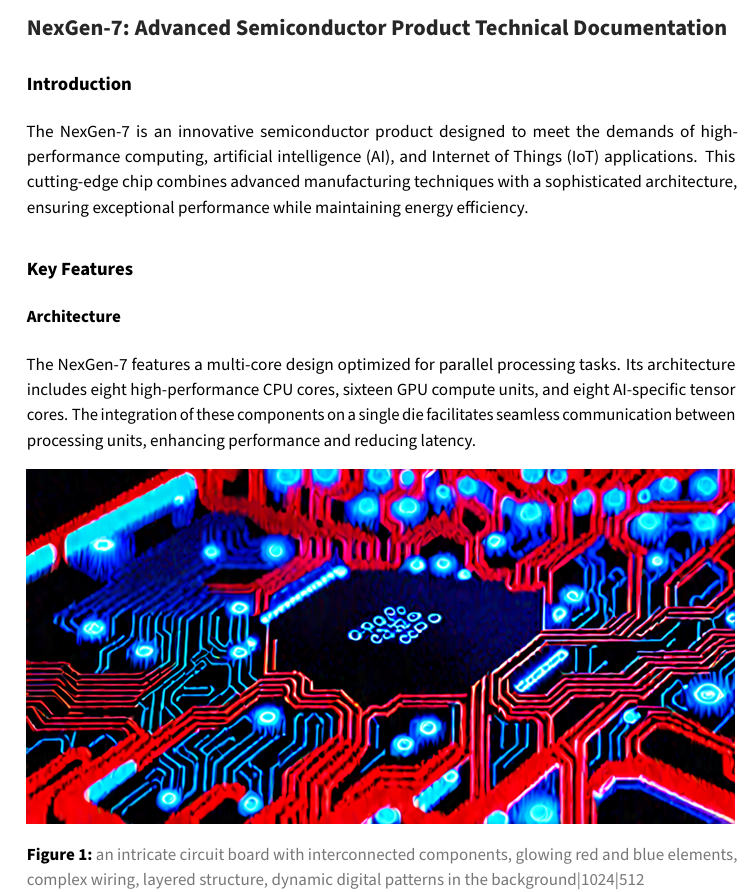
\includegraphics[width=1\linewidth]{pdf-example.png}
\caption{Sample of an AI-generated PDF artifact to be used in a themed
scenario}\label{fig:artifact-document-example}
\end{figure}

Of course, the process can be simplified to exclusively generating
images. For example, the images in \autoref{fig:artifact-image-example}
were generated by instructing DeepSeek-R1 to provide a list of image
generation prompts related to semiconductor manufacturing. These were
then passed to SDXL 1.0.

\begin{figure}[h]
\centering
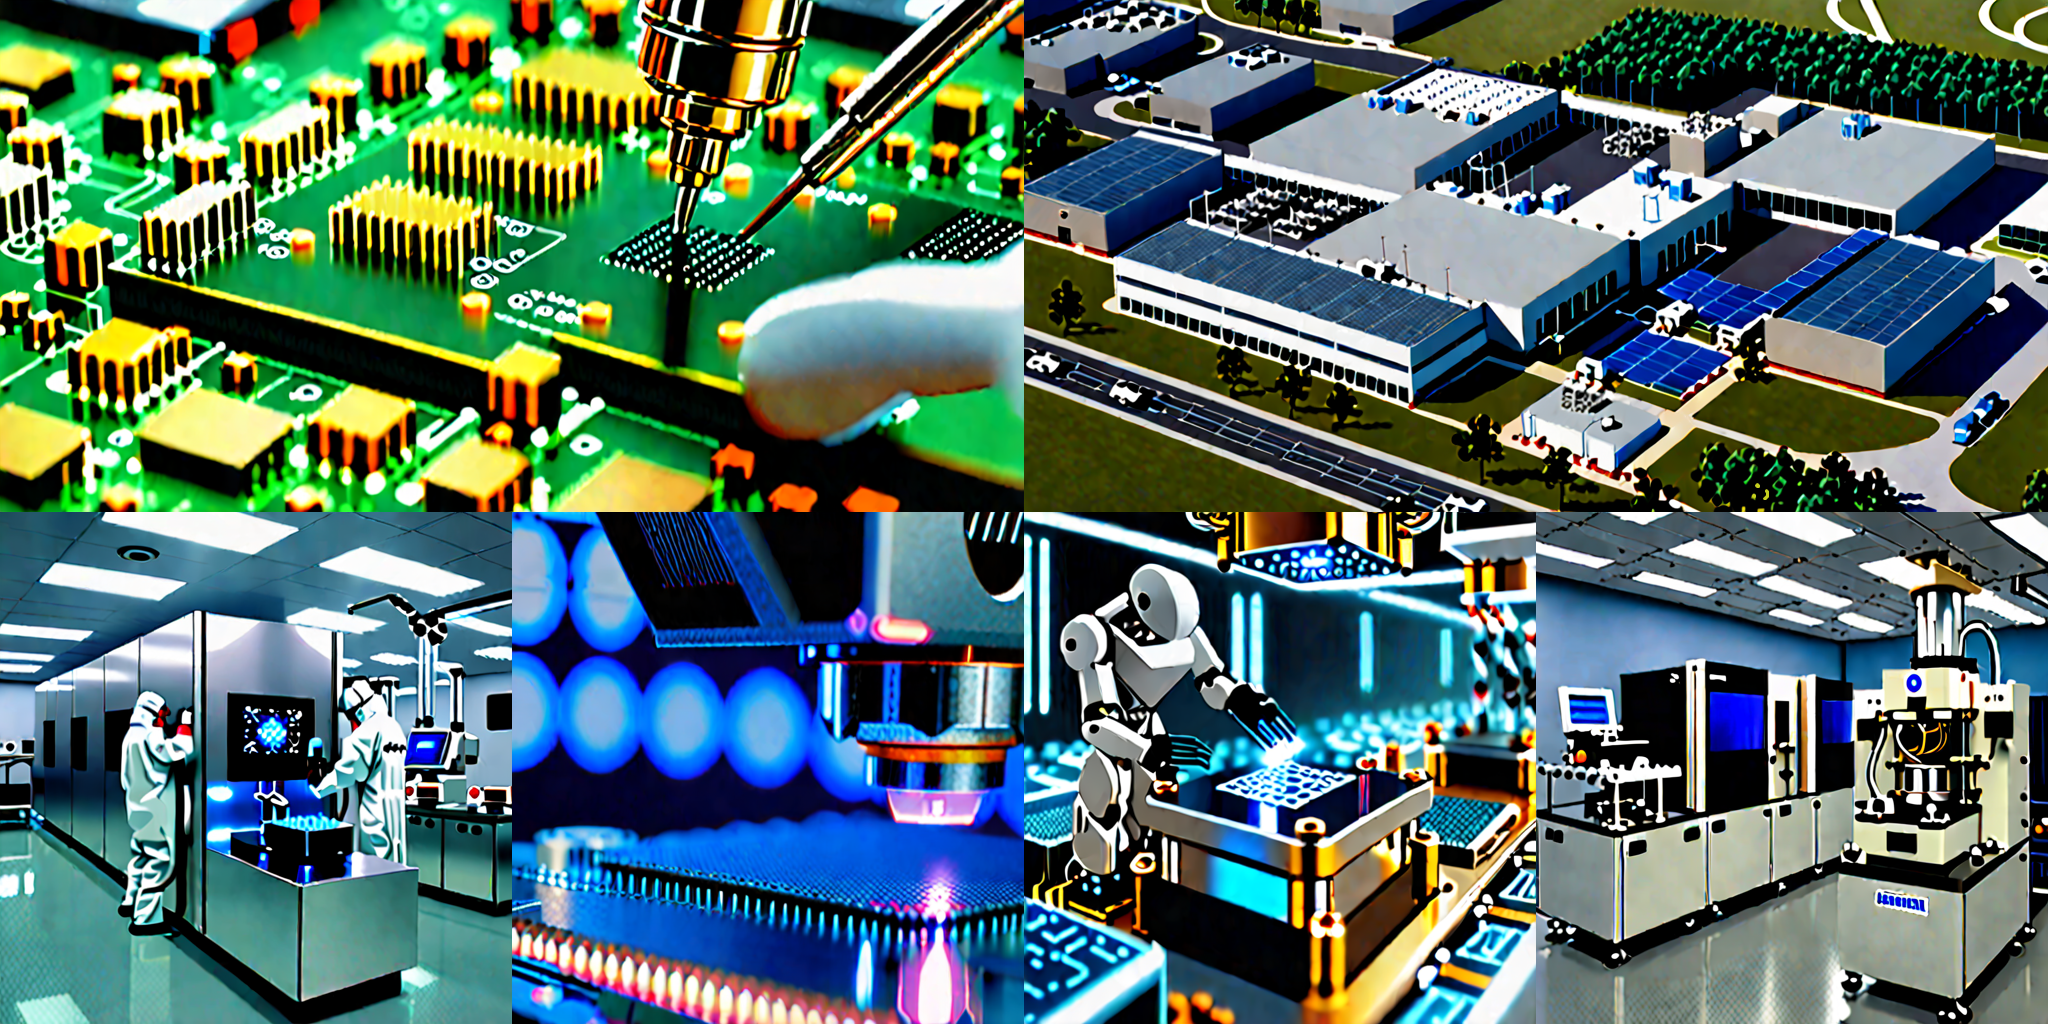
\includegraphics[width=1\linewidth]{collage.png}
\caption{Collage of AI-generated images for use in a themed
scenario}\label{fig:artifact-image-example}
\end{figure}

Finally, we noted that the Data Leakage Case lacks background email
conversations. Email conversations as part of a scenario can be divided
into three categories:

\begin{itemize}
\tightlist
\item
  Emails that are relevant to the focus or topic of the scenario, such
  as corporate espionage
\item
  Emails that are irrelevant to the scenario but are consistent with the
  persona included as part of the scenario, such as benign emails to
  coworkers
\item
  Emails wholly irrelevant to the scenario, such as marketing or spam
  emails
\end{itemize}

To generate these emails, DeepSeek-R1 was prompted to generate email
conversations according to the three email categories above in a
well-structured format that could easily be converted to a valid
\passthrough{\lstinline!.eml!} file using the Python standard library.
DeepSeek-R1 was provided details such as the email address to use when
sending/receiving emails and the corporate email domain to use in
relevant emails. An excerpt of a sample email conversation can be seen
in \autoref{fig:artifact-email-example}.

\begin{figure}[h]
\centering
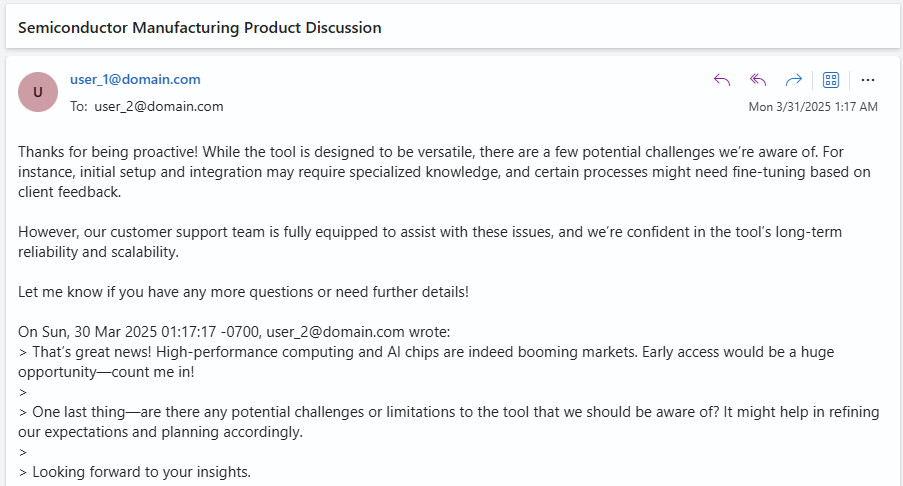
\includegraphics[width=1\linewidth]{email_snippet.png}
\caption{Sample of an AI-generated email
conversation}\label{fig:artifact-email-example}
\end{figure}

Consistent with the architectural diagram depicted in
\autoref{fig:architecture-full-a}, the use of generative AI in AKF is
almost entirely decoupled from other parts of the framework and can be
applied outside of synthesizer contexts. Although the three-step process
to generate the artifacts above was carried out manually, the same
process could be implemented in standalone modules in the AKF library.
There are various libraries and solutions for interfacing with Ollama
and ComfyUI through Python; these libraries could be leveraged in such
an implementation.

\section{Using LLMs for high-level
scenarios}\label{using-llms-for-high-level-scenarios}

The prior section addressed the challenge of generating individual
artifacts for a dataset. However, there remains the challenge of using
these artifacts to generate a cohesive scenario. That is, with an
overall scenario theme or goal in mind, what specific synthesizer
actions should be taken to construct a dataset that adheres to that
theme? Even with the automation routines provided by AKF and individual
artifacts prepared (whether created manually or using generative AI), it
still takes time to define a scenario, especially one that involves many
different types of actions that cannot easily be simplified into a small
number of synthesizer actions. This is true even with a simplified
declarative syntax.

One solution is to provide the details of AKF's declarative syntax to an
LLM and instruct it to generate valid declarative scripts. In
particular, there are two features of the declarative syntax that lends
itself well to this process:

\begin{itemize}
\tightlist
\item
  The role of each module is well-defined and corresponds one-to-one to
  a specific action that a human might take, such as visiting a set of
  websites.
\item
  The expected inputs for each module are well-defined, as they are
  documented by the required Pydantic argument model for each module.
\end{itemize}

To explore this, an instance of
\passthrough{\lstinline!deepseek-r1:32b!} was provided with the
following information. (The actual prompts and outputs used to derive
the content in this section are included with the scenario examples for
the AKF Windows agent.)

\begin{itemize}
\tightlist
\item
  An overview of the purpose of the declarative syntax.
\item
  The overall structure of the syntax, such as the required top-level
  keys and the structure of individual actions under the
  \passthrough{\lstinline!actions!} key.
\item
  A Markdown-formatted table in which each row contains the name,
  description, and arguments of available modules. Except for the
  arguments column, the table was equivalent to
  \autoref{tbl:akf-declarative-modules}.
\item
  A prompt delimited by \passthrough{\lstinline!<scenario\_prompt>!}
  tags that should be used to build the overall scenario.
\end{itemize}

We observed that this information was generally sufficient for
DeepSeek-R1 to ``understand'' the AKF syntax, allowing it to generate
simple declarative scripts. Although the prompt containing this
information was manually written, much of the prompt could be used as a
template and substituted with the contents of automatically generated
documentation. For example, the table of available modules could be
generated through existing code metadata, such as the contents of
docstrings and Pydantic argument models.

For example, DeepSeek-R1 was directed to create a simple scenario where
a user visited news-related websites with Microsoft Edge and
entertainment-related websites with Google Chrome, ensuring that the
machine went through multiple power cycles throughout the scenario.
Although DeepSeek-R1 was not provided with examples specific to invoking
the \passthrough{\lstinline!chromium\_visit\_urls!} module, it correctly
constructed an argument dictionary containing several thematically
consistent websites for both browsers. Additionally, it correctly used
the \passthrough{\lstinline!vbox\_start\_machine!} and
\passthrough{\lstinline!vbox\_stop\_machine!} actions to perform
multiple power cycles.

However, DeepSeek-R1 struggled to understand the interactions between
related modules without additional guidance. For example, it did not
infer that the use of the \passthrough{\lstinline!vbox\_stop\_machine!}
and \passthrough{\lstinline!vbox\_start\_machine!} actions required that
a hypervisor instance had been previously created using
\passthrough{\lstinline!vbox\_start!}. Even when the module descriptions
were modified to state these requirements explicitly, it continued to
invoke \passthrough{\lstinline!vbox\_start\_machine!} without a
preceding \passthrough{\lstinline!vbox\_start!} action. In contrast,
DeepSeek-R1 appeared to understand that
\passthrough{\lstinline!chromium\_service\_start!} should be called
before calling any other Chromium-related modules, even when this
requirement was not stated. Indeed, the Chromium-related modules
support, but do not require, the use of
\passthrough{\lstinline!chromium\_service\_start!} to explicitly connect
to the Chromium RPyC subservice.

Additionally, DeepSeek-R1 would sometimes invoke modules incorrectly,
such as providing arguments that did not exist or invoking them with the
incorrect name. One notable example was that it incorrectly used
\passthrough{\lstinline!vbox\_start\_machine!} to both start and stop
the virtual machine, adding an erroneous
\passthrough{\lstinline!action: "stop"!} argument when stopping the
virtual machine. In some cases, DeepSeek-R1 deviated significantly from
the declarative syntax and used keys that did not exist, such as
specifying module arguments outside of the
\passthrough{\lstinline!args!} dictionary.

Despite these issues related to correctness, it was clear that
DeepSeek-R1 could convert abstract prompts into a sequence of actions
based on the available modules provided. Much like using declarative
scripts as a starting point for imperative scripts, these outputs can
likely be used as a starting point for more complex declarative scripts.
Furthermore, these issues could be alleviated by improving the details
of the prompt, such as providing specific examples of module usage and
the overall results they cause. In particular, DeepSeek-R1 is a
reasoning model, which means that it ``thinks out loud'' before
responding; the model's thoughts could be used to identify and eliminate
vagueness or uncertainty in the provided prompt. Writing precise,
detailed documentation with this LLM-oriented pipeline in mind could
further improve the quality of generated outputs.

As more declarative modules and functionality are added to AKF, it is
clear that LLMs can significantly accelerate converting abstract
scenario goals into a script that will carry out the necessary actions
to fulfill these goals. This is especially true given continuing
advancements in generative AI, which are likely to improve the
performance of these models in adhering to specific instructions.

\chapter{Future work}\label{chapter-eight}

AKF was built with the expectation that it would be easy to maintain,
develop, and extend. Indeed, there are several use cases that AKF does
not fulfill as of writing, primarily due to time constraints. Future
work related to AKF can be characterized as either tasks that integrate
cutting-edge advancements to implement new features or tasks that extend
or improve existing functionality. In particular, \autoref{open-ended-automation-with-ai} describes the application of
recent AI developments towards addressing tasks relevant to forensic
dataset development; the remaining sections focus on extending existing
concepts in AKF.

\section{Open-ended automation with
AI}\label{open-ended-automation-with-ai}

During the development of AKF, OpenAI announced the release of Operator,
an ``agent'' capable of automating tasks on webpages using natural
language prompts \cite{openaiIntroducingOperator2025}. Rather than
using a browser automation framework like Playwright or Selenium, it
leverages its own browser to interact with webpages. Users can provide
Operator with a high-level goal, which it then converts to concrete
actions on its browser to achieve that goal.

OpenAI provides an example in which Operator searches Allrecipes for a
clam linguine recipe and then orders the ingredients for the linguine
through Instacart. Various sensitive actions during this process are
delegated to the user to complete, such as inputting payment information
or logging into a service. Operator is also capable of identifying
ambiguity in a task and prompting the user for clarification, such as
asking which store to use for ordering items through Instacart. This
example demonstrates multiple notable features that are relevant to
forensic synthesizers; in particular, it demonstrates the ability to
both \emph{interpret} and \emph{interact} with arbitrary GUIs, as well
as the ability to convert human prompts into a sequence of automated
actions that may change as the agent discovers new information or
encounters unexpected issues.

It is powered by what OpenAI calls its ``Computer-Using Agent,'' or CUA,
which is trained to interact with a virtual machine by accepting natural
language and a screenshot of a virtual monitor
\cite{openaiComputerUsingAgent2025}. It leverages OpenAI's GPT-4o
model, following a three-step process in which it analyzes screenshots
of the virtual desktop, conducts reasoning to determine the necessary
steps to achieve a task (using prior context), and executes actions on
the virtual machine. OpenAI notes that CUA can reliably perform simple
tasks that a human would usually perform, such as navigating to specific
categories of websites or repeating UI interactions. However, it
struggles with some interfaces it has not encountered before and tends
to be inefficient or hallucinate on more complex tasks.

The challenge of automating open-ended tasks through AI is not new.
Multiple benchmarks (mentioned in OpenAI's articles), including
WebVoyager, WebArena, and OSWorld, were developed in early 2024 to
provide examples of typical webpage and OS interaction tasks performed
by humans
\cite{zhouWebArenaRealisticWeb2024,heWebVoyagerBuildingEndtoEnd2024,xieOSWorldBenchmarkingMultimodal2024}.
CUA is stated to achieve state-of-the-art results in these benchmarks,
representing the current ability of AI to address open-ended tasking.
Although CUA has clear limitations and falls well behind human
performance on these benchmarks, Operator demonstrates significant
progress in the ability of AI models to replicate actions that are often
performed by real users. Even in its current state, CUA can likely
automate the ``simple'' tasking involved in generating background noise
for forensic datasets, such as browsing news sites, interacting with
social media platforms, and more.

In the near future, works similar to CUA or Operator will likely be
capable of fully automating human actions as part of a larger scenario
with high reliability and accuracy. Improvements to interacting with
previously unseen GUI-based applications will increase the variety and
complexity of actions that can be automated. These capabilities are
extremely valuable in synthetic dataset generation, as they dramatically
reduce the time needed to implement artifact generation functionality
for novel technologies or developments.

What do these developments mean for ``conventional'' synthesizer
architectures, which depend on scripts instead of natural language?
First, the verbosity of writing a script and passing it to a synthesizer
is still valuable, particularly in contexts where the non-determinism
and opacity of an AI model may not be acceptable. Several works have
described the non-deterministic nature of LLMs in multiple distinct
tasks
\cite{astekinExploratoryStudyHow2024,songGoodBadGreedy2024,ouyangEmpiricalStudyNonDeterminism2025},
which negatively impacts the reproducibility of results -- an important
quality of forensic datasets as described by Grajeda et al.
\cite{grajedaAvailabilityDatasetsDigital2017}.~Non-determinism is
often acceptable in educational contexts so long as the actions taken by
the model are logged and can be verified after the fact. However, the
development of datasets for research and tool validation may require
that a set of instructions always generates the same dataset every time,
ensuring reproducibility from the instructions alone.

Second, these developments are not \emph{incompatible} with synthesizers
and should instead be seen as an option to complement them. The
capabilities provided by Operator could likely be built into AKF as part
of its internal library or an OS-specific agent, providing users with
access to both verbose imperative/declarative scripts as well as simpler
natural language prompts when automating actions and building scenarios.
Additionally, these agents cannot (currently) act as a substitute for
physical artifact generation, in which the underlying filesystem or disk
image must be edited to fulfill a particular task. Since these agents
are trained to work with ``live'' operating systems and applications,
they are likely unsuitable for automating physical operations on
filesystems and disk images.

\section{Alternative platform
support}\label{alternative-platform-support}

One future extension is implementing support for other desktop
environments, such as Mac and Linux. At a high level, this requires
implementing artifact generation methods described in \autoref{chapter-four} for each platform.

Consistent with AKF's focus on using existing automation frameworks
through agents to implement application-specific functionality, much of
the effort for supporting other platforms requires writing and deploying
a new OS-specific agent. Much of the code and overall design can be
inherited from the Windows agent, enabled through the portability of
Python and the lack of OS-specific assumptions made by RPyC. Certain
automation frameworks may have significant cross-platform support (such
as Playwright and \passthrough{\lstinline!pywinauto!}, which support
Windows, Mac, and Linux), though implementing functionality for other
applications may require more effort.

Implementing logical agentless generation through VirtualBox is likely
straightforward, mainly because Oracle supports Guest Additions on MacOS
and many Linux distributions. Similarly, the physical artifact
generation implemented in AKF for FAT32 and NTFS (the most common
filesystems for Windows) is likely extensible to other disks, such as
ext4 (the default for modern Linux distributions). This is because
\passthrough{\lstinline!dfvfs!}, the library used to support disk image
and filesystem editing, supports many filesystems, partitioning
standards, and disk images commonly used by other operating systems.

The primary challenge in cross-platform support lies in accounting for
artifacts or mechanisms unique to other operating systems. Some
features, such as PowerShell/WinRM and Bash/SSH, are analogous between
Windows and Unix-based systems and can be adapted accordingly. However,
some concepts are truly unique to an operating system, such as
performing modifications to the operating system through Windows
registry keys, and may require more effort to adapt the same outcomes to
other platforms.

\section{Additional interface
implementations}\label{additional-interface-implementations}

Another future extension involves developing new concrete
implementations of AKF interfaces using other technologies that may have
better support for specific host and guest platforms. AKF currently
provides a VirtualBox implementation of the hypervisor-agnostic
interface provided as part of \passthrough{\lstinline!akflib!}, largely
depending on the VirtualBox Guest Additions software to function.
Indeed, this is the approach taken by virtually all prior synthesizers
that require virtualization; existing work leveraging VirtualBox to
implement automation functionality has contributed significantly to its
adoption across many synthesizers, including AKF.

However, prior synthesizers have also considered KVM/Qemu and VMWare as
hypervisors; in particular, Forensig2 leveraged Qemu as its
virtualization platform \cite{mochForensicImageGenerator2009}.
Several considerations exist for using other synthesizers, including
support on different host platforms, performance, and available
functionality. For example, Hwang et al.~compared the performance and
low-level features of multiple hypervisors, including Hyper-V, KVM/Qemu,
and VSphere, finding significant variability between these hypervisors
when running workloads and applications
\cite{hwangComponentbasedPerformanceComparison2013}. It may be the
case that specific scenarios or host machines are better suited for
other hypervisors or even a multi-hypervisor environment. It is worth
noting that VMWare has guest-specific software similar to the VirtualBox
Guest Additions; multiple Python libraries exist for interacting with
guests on VSphere, such as \passthrough{\lstinline!pyvmomi!}
\cite{VmwarePyvmomi2025}.

Similarly, rather than create new implementations of existing
interfaces, it may also be worth building new interfaces entirely. One
example is the implementation of agents in languages other than Python.
Using non-Python agents may cover needs for specific tasks (such as
actions that can be automated using a library for which no Python
equivalent exists) or specific deployment restrictions (such as avoiding
extraneous data due to synthesizer operation). In general, the
implementation for an agent can be written in any language, so long as a
corresponding Python API exists; the burden would be on the author to
handle any communication or discrepancies across disparate languages,
such as writing a TCP-based protocol for issuing commands.

\section{Distribution}\label{distribution}

One notable development of prior synthesizers not implemented as part of
AKF is the various improvements to the distribution of generated
datasets, particularly in environments with limited bandwidth or storage
space. AKF primarily addresses challenges in the \emph{creation} of
forensic datasets rather than their \emph{distribution}. This section
addresses prior efforts to reduce the size of forensic datasets and how
they could be integrated into AKF in the future.

The size of forensic datasets can be trivially reduced in various ways.
For example, a full forensic dataset can be compressed using a standard
algorithm such as LZMA. Specific core outputs, such as disk images, can
be stored in a dynamically expandable image format such as VDI or VHD.
Such formats only use as much space as is currently used on the disk
image itself, even if the size reported to the operating system is much
larger. These reductions are ``lossless'' in that they can be reversed
to reflect what a forensic analyst would encounter using real hardware.

However, more aggressive ``lossy'' reductions can be performed to
further reduce dataset size. These can be broadly described as one of
two approaches -- either irrelevant data is outright removed, or the end
user must take additional effort to finish preparing the forensic
scenario for use after downloading relevant files (which are
significantly smaller than the finished forensic dataset itself). The
first approach reduces realism in exchange for a smaller dataset size;
the second approach requires additional processing time in exchange for
reduced network transfer sizes.

The first method describes the process of simply removing data that is
not deemed to be relevant for educational or research purposes. For
example, suppose an instructor is interested in demonstrating only the
recovery and analysis of SQLite databases in Chrome's AppData directory.
For this scenario, there is no need to include files from most other
directories on the filesystem. One option for achieving this is to use a
logical disk image format, such as the AD1 format, which is a collection
of files (much like a ZIP archive) instead of a collection of physical
disk units (like a standard disk image).

A more notable approach to removing irrelevant information is described
by Russell et al.~as part of their work developing SFX
\cite{russellForensicImageDescription2012}. Their approach,
described as ``partition squeezing,'' is based on the idea that the
contents of files irrelevant to an educational scenario can be truncated
to the size of a single filesystem cluster or block. (In some
filesystems, a file can be further truncated to fit entirely within
filesystem metadata structures, such as resident files in NTFS.) This
preserves the file and directory structure of the overall filesystem
(thus preserving realism) while also removing data that is unlikely to
be useful to students performing analysis. Thus, the educational value
of the image remains the same, even if some data is missing. Russell et
al.~note that additional space can be saved by replacing irrelevant
files with hard links to other files, particularly those deep within the
filesystem that are highly unlikely to be analyzed in detail by
students. This entirely eliminates the original contents of the file
while preserving most of its attributes.

The use of logical images and partition squeezing, of course, is not
suitable in all cases. In particular, logical images generally do not
include slack or unallocated space. The partition squeezing approach
destroys data that may be required for certain forensic analysis tools
to function, as well as data that might be of interest to users of the
dataset in other research or educational contexts than initially
intended.

AKF does not provide any functionality for directly generating logical
images or performing partition squeezing. However, generating logical
images is relatively straightforward using a publicly available tool
such as FTK Imager, so long as the scenario developer is aware of
relevant directories that should be included -- a process that might
occur with AKF's reporting features in mind. Partition squeezing could
be achieved by leveraging the filesystem-aware functionality of
libraries such as \passthrough{\lstinline!libtsk!} and
\passthrough{\lstinline!dfvfs!}, which is used as part of AKF's physical
planting techniques described in \autoref{akf-implementation}. However, a more straightforward approach is to
mount the filesystem and truncate all irrelevant files to the size of a
single block or cluster. Such functionality could be implemented either
in AKF or as part of a wholly independent tool.

The second method describes various techniques in which end users must
take additional actions after downloading relevant materials before a
forensic dataset is ready for use. One example described by Scanlon et
al.~is the use of ``evidence packages,'' in which users are provided
with a base image of a single operating system that can be reused to
build multiple forensic datasets through EviPlant
\cite{scanlonEviPlantEfficientDigital2017}. After a scenario
developer has finished creating artifacts (whether manually or through a
synthesizer), they can use EviPlant's ``diffing'' tool to determine and
extract differences between the base image and the developer's current
disk state. These differences can be distributed to users, who can then
use EviPlant's ``injection'' tool on the previously distributed base
image to recreate the final disk image.

This approach can described more generally as ``differential imaging'',
in which only differences from some initial files are saved and
transmitted to users. These differences are often significantly smaller
than the disk images they are designed to build and are much easier to
distribute than complete disk images. (This is very similar to the
approach used by Vagrant to distribute and prepare reproducible virtual
machines, as described in \autoref{setup-and-basic-usage}.) In exchange, each user must spend additional
processing time before the image can be used for analysis. EviPlant's
injection tool operates through a combination of logical and physical
planting, which requires time, software, and resources that are not
required when using and distributing complete disk images. This is an
acceptable cost in some cases; for example, not all students in a remote
classroom may have high-speed internet, limiting the size of files that
can be distributed. Again, although AKF does not implement differential
imaging, this functionality can likely be implemented as part of an
independent tool or module.

\section{Mobile synthesis}\label{mobile-synthesis}

Finally, although well outside the scope of this thesis, there is also
the challenge of building a synthesizer for non-desktop platforms,
particularly mobile devices. For many people, mobile devices are the
primary means of interacting with the digital world, causing them to
play a unique role in investigations
\cite{chernyshevMobileForensicsAdvances2017}. Mobile devices can
contain data from many facets of one's life, including text messages,
location history, images, application logs, and other information that
can provide insight into an individual's actions during a period of
interest \cite{sutiknoCapabilitiesCellebriteUniversal2024}. This
information can be combined with other investigative methods, such as
desktop and conventional forensics, to form a better understanding of a
larger scenario.

Naturally, this means that there is a need for mobile datasets in
digital forensics, as well. Grajeda et al.~identify a small number of
existing mobile dataset collections, including those containing Android
malware, Android application files, and smartphone disk images
\cite{grajedaAvailabilityDatasetsDigital2017}. However, these
datasets are far less common than their desktop counterparts. Compared
to the hundreds of desktop disk images hosted on Digital Corpora and
CFReDS, there are only around 25 mobile disk images on the same
platforms. A mobile-specific survey conducted by Gonçalves et al.~in
2022 found not only a low availability of mobile images but also a lack
of background noise and recent applications that would be present in a
modern investigation \cite{goncalvesRevisitingDatasetGap2022}.

There has been limited work in developing forensic synthesizers for
mobile platforms. Two notable examples are FADE
\cite{ceballosdelgadoFADEForensicImage2022}, developed by Delgado et
al.~in 2022, and a branch of ForTrace developed by Demmel et al.~in 2024
\cite{demmelDataSynthesisGoing2024}. FADE operates primarily through
physical artifact generation, which it achieves by extracting and
mounting partitions from an emulated, rooted Android device using the
Android Debug Bridge. It then modifies application-specific database
files to create artifacts such as phone call entries and text messages.

In contrast, Demmel et al.~generate data using a logical agentless
approach, using a tool called AndroidViewClient (AVC) to send keypresses
and touch gestures \cite{demmelDataSynthesisGoing2024}. Unlike
VMPOP, which uses hardcoded mouse movements to click on GUI-based
elements, this framework leverages AVC to expose all interactable UI
elements and programmatically ``touch'' these elements once the desired
element has been found. This allows it to implement more complex
application-specific functionality, such as using WhatsApp and opening
Google Chrome.

There has also been broader work in automating actions as part of
testing pipelines for Android applications
\cite{janickiObstaclesOpportunitiesDeploying2012,nagowahNovelApproachAutomation2012,linares-vasquezHowDevelopersTest2017},
though these primarily address application-specific actions, rather than
automating actions across the entire device. Of note is the lack of
iOS-relevant synthesizer functionality, perhaps due to the greater
difficulty of working on a closed-source operating system with fewer
options for exposing internal functionality.

It is possible that \emph{some} of AKF's architecture could be adapted
to support mobile dataset generation, primarily by interacting with
Android emulators and existing developer tools. However, the isolation
around individual Android applications suggests that it may be difficult
to use a logical agent-based approach to automating application
activity; a Python agent running as an application is unlikely to have
full filesystem access on a non-rooted device. For simple
application-specific artifacts, using physical techniques and editing
artifacts in an application's allocated directory may be more effective.
Much like Windows, however, Android applications may generate both
application-specific artifacts and system artifacts (such as system
logs) located elsewhere in the filesystem.

More research is needed to determine viable options for constructing
Android datasets. This is especially true for iOS, for which there are
significantly fewer resources.

\chapter{Conclusion}\label{chapter-nine}

Public forensic datasets are invaluable to advancing research and
education throughout digital forensics. However, high-quality datasets
are presently few in number and may not fit specific needs, motivating
the development of new datasets. Constructing these datasets by hand is
time-consuming and prone to errors, yet it continues to be the primary
method through which new datasets are made. In turn, there is a need for
synthesizers, which allow users to create datasets using high-level
scripting languages that can automate many common actions. Although
prior synthesizers have addressed the creation of specific forensic
artifacts, there are still opportunities to improve their flexibility
and usability while promoting their usage throughout the forensic
community.

AKF, the \emph{automated kinetic framework}, introduces a modern
approach to forensic synthesis through a modular architecture focusing
on sustained development and community adoption. It provides significant
advancements in artifact generation, logging and validation, and the
overall construction of new scenarios. It improves artifact generation
by integrating numerous technologies not leveraged by prior
synthesizers, greatly simplifying the implementation of the overall
architecture without compromising the breadth of features available
through the framework. By using a centralized logging architecture and
the CASE ontology, AKF is able to generate detailed, queryable metadata
of the datasets it generates, allowing users to quickly identify
artifacts of interest in a dataset. AKF also exposes a simple
declarative syntax for generating artifacts, allowing users to develop
scenarios without writing code using the underlying Python
libraries.~Finally, it provides a demonstration of using LLMs to further
streamline scenario development, both when constructing individual
artifacts and when building a complete scenario.

Although there are still limitations to what AKF can accomplish,
numerous opportunities exist to leverage existing and emerging
technologies to extend the framework. These contributions have been made
in the hope that they will advance research and education throughout
digital forensics, allowing the community to fill known gaps in public
datasets.

% == End thesis content


%glossary & acronym lists
% \printglossary[type=\acronymtype]
% \printglossary

% \nocite{*}
\singlespacing
\printbibliography[heading=bibintoc, title={Bibliography}]
% \bibliography{thesis_bib}

\doublespacing
\appendix

\appendix

\chapter{Architectural diagrams}\label{appendix-a}

\autoref{fig:mini-full} is a complete representation of the AKF
architecture, excluding labels. The remaining diagrams in this appendix
chapter focus on individual modules in greater detail;
\autoref{fig:mini-full} is intended to help the reader understand the
relationships between individual sub-diagrams, which contain the labels
omitted from this figure.

The following conventions are used for all architectural figures
throughout this thesis, including those below:

\begin{itemize}
\tightlist
\item
  Elements with a \textbf{solid border} refer to AKF submodules, which
  contain processing logic.
\item
  Elements with a \textbf{dotted border} refer to inputs, such as
  scripts and images, that should be used to construct a dataset.
\item
  Elements with a \textbf{dashed border} refer to outputs, such as disk
  images and memory dumps, that should be included with a complete
  dataset.
\end{itemize}

In general, colored boxes refer to a distinct module. The sole exception
is the \emph{translation unit} (colored green), which is distinctly
colored from other submodules due to its complexity.

\begin{figure}[h]
\centering
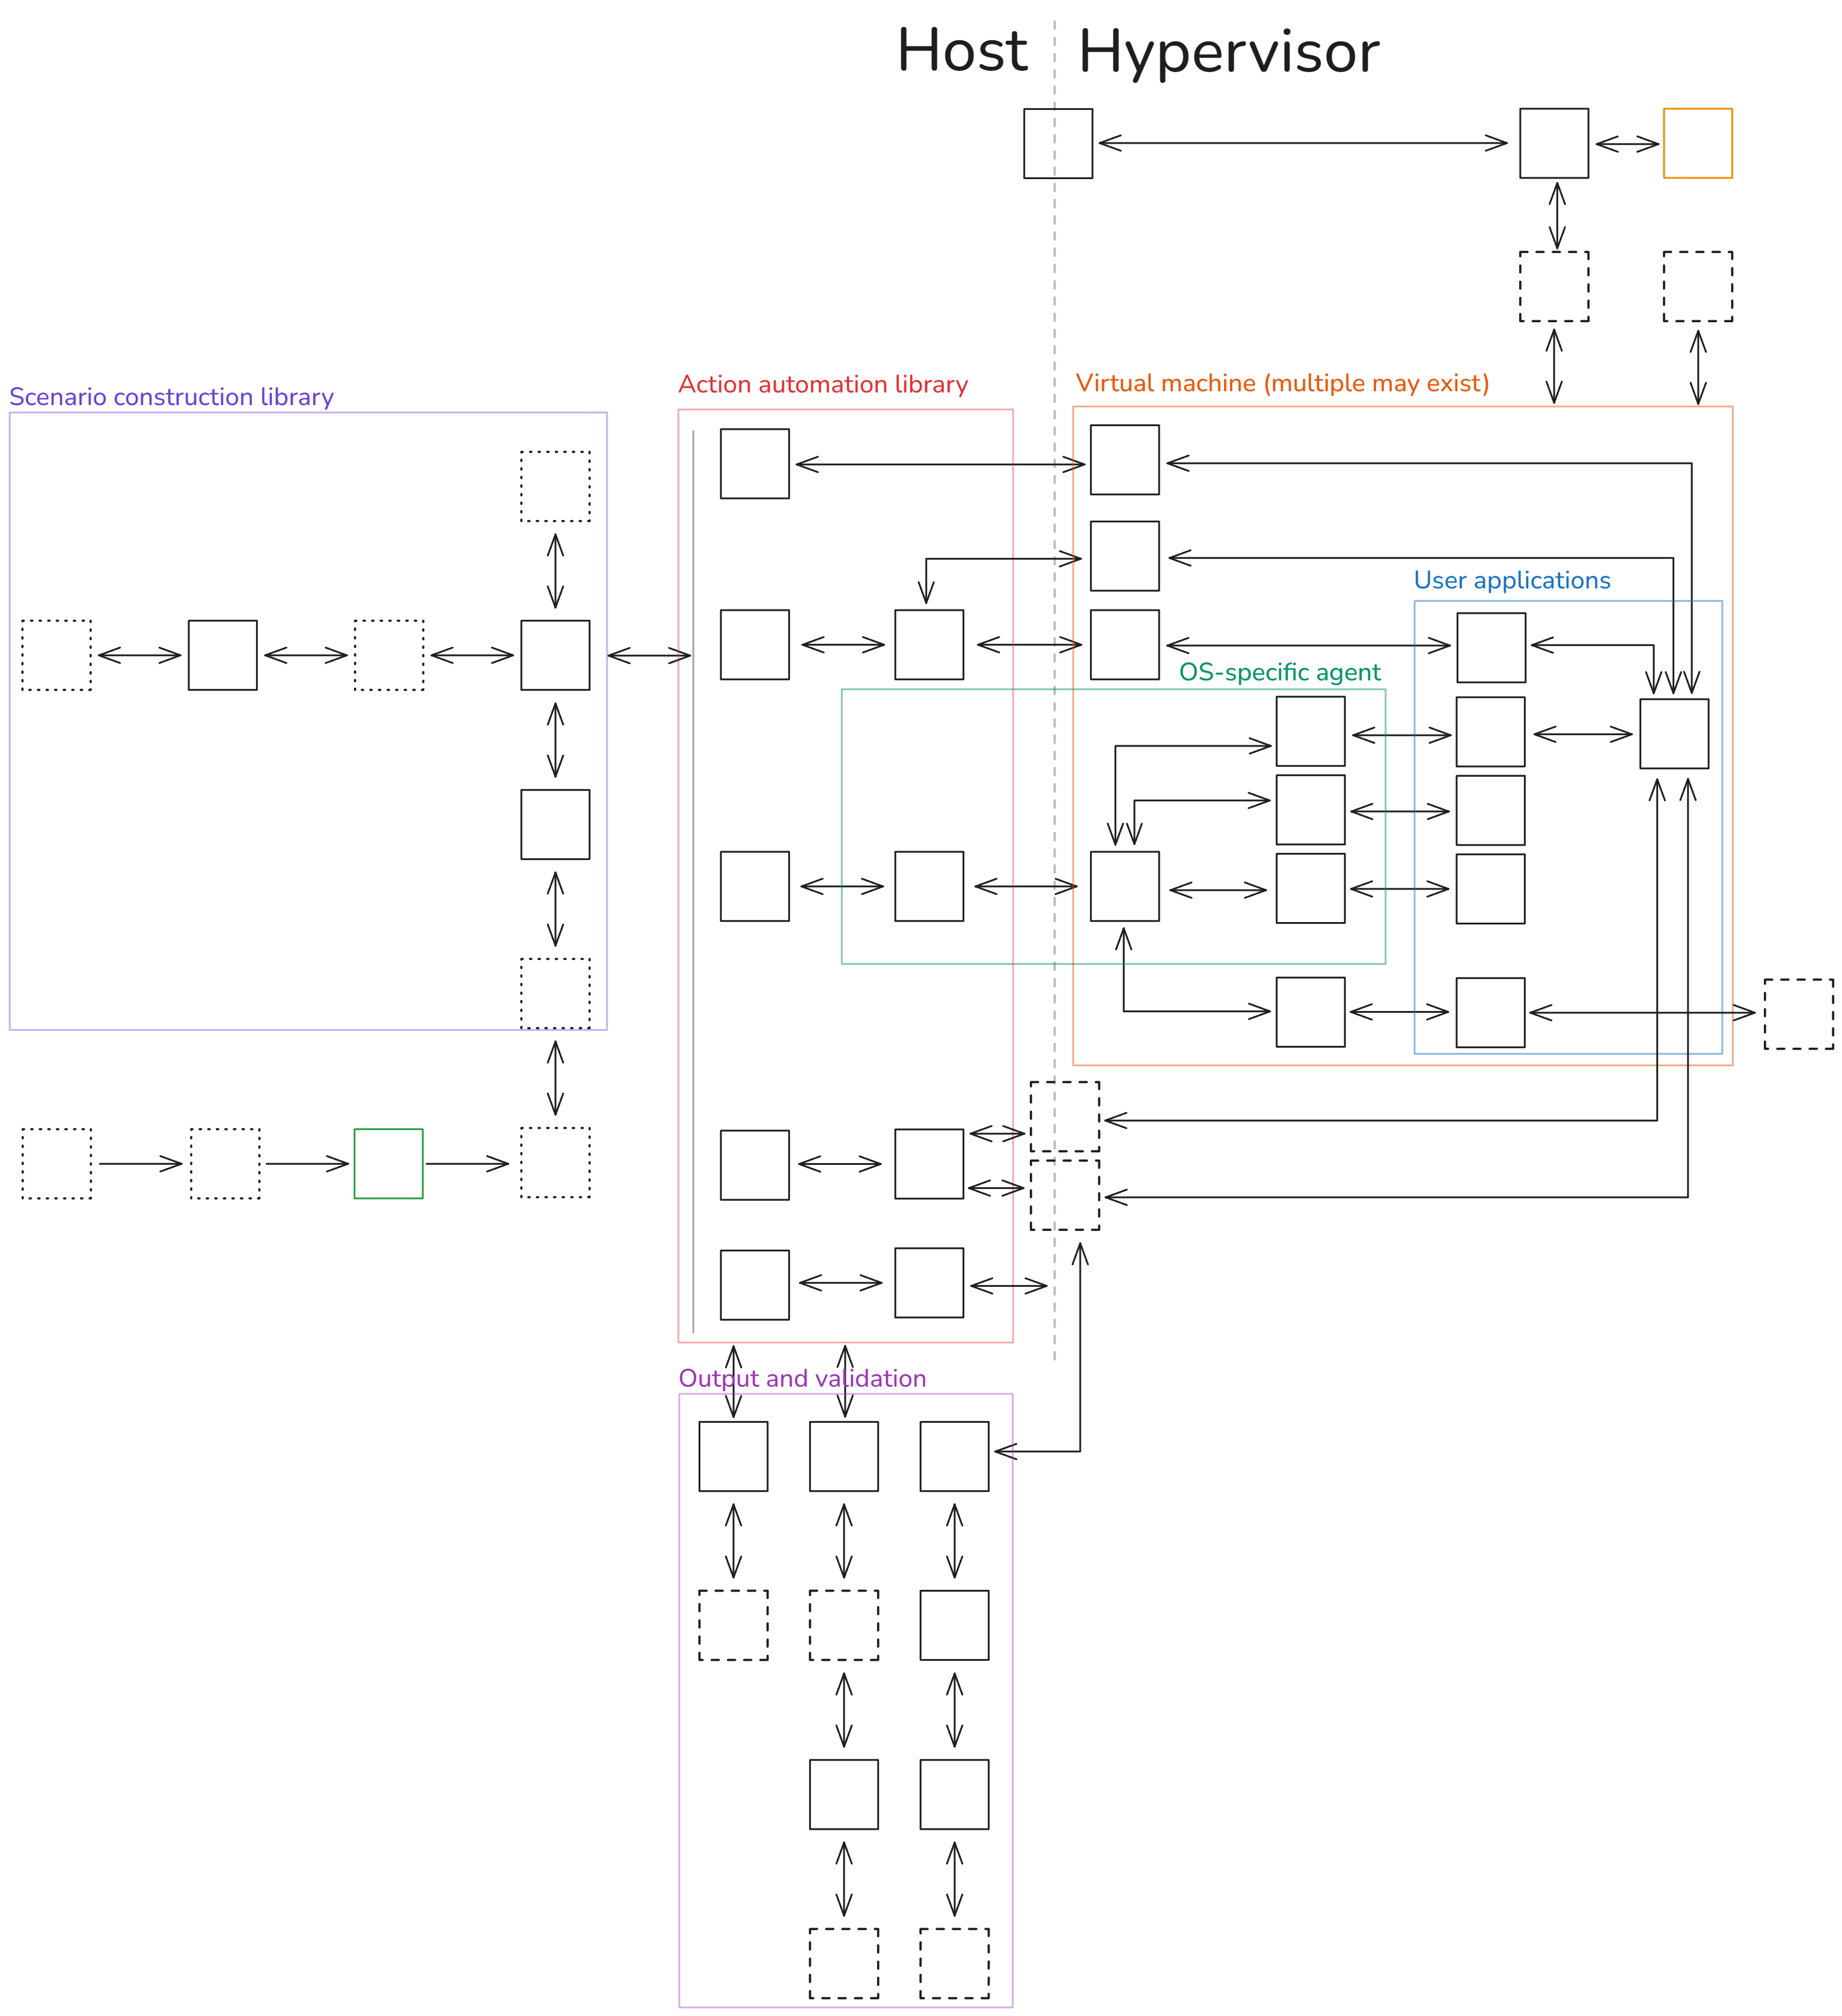
\includegraphics[width=1\linewidth]{mini-architecture-full.png}
\caption{Complete diagram of AKF modules without
labels}\label{fig:mini-full}
\end{figure}

The action automation library, described throughout \autoref{chapter-four}, is depicted in \autoref{fig:architecture-full-b}.

\begin{figure}[h]
\centering
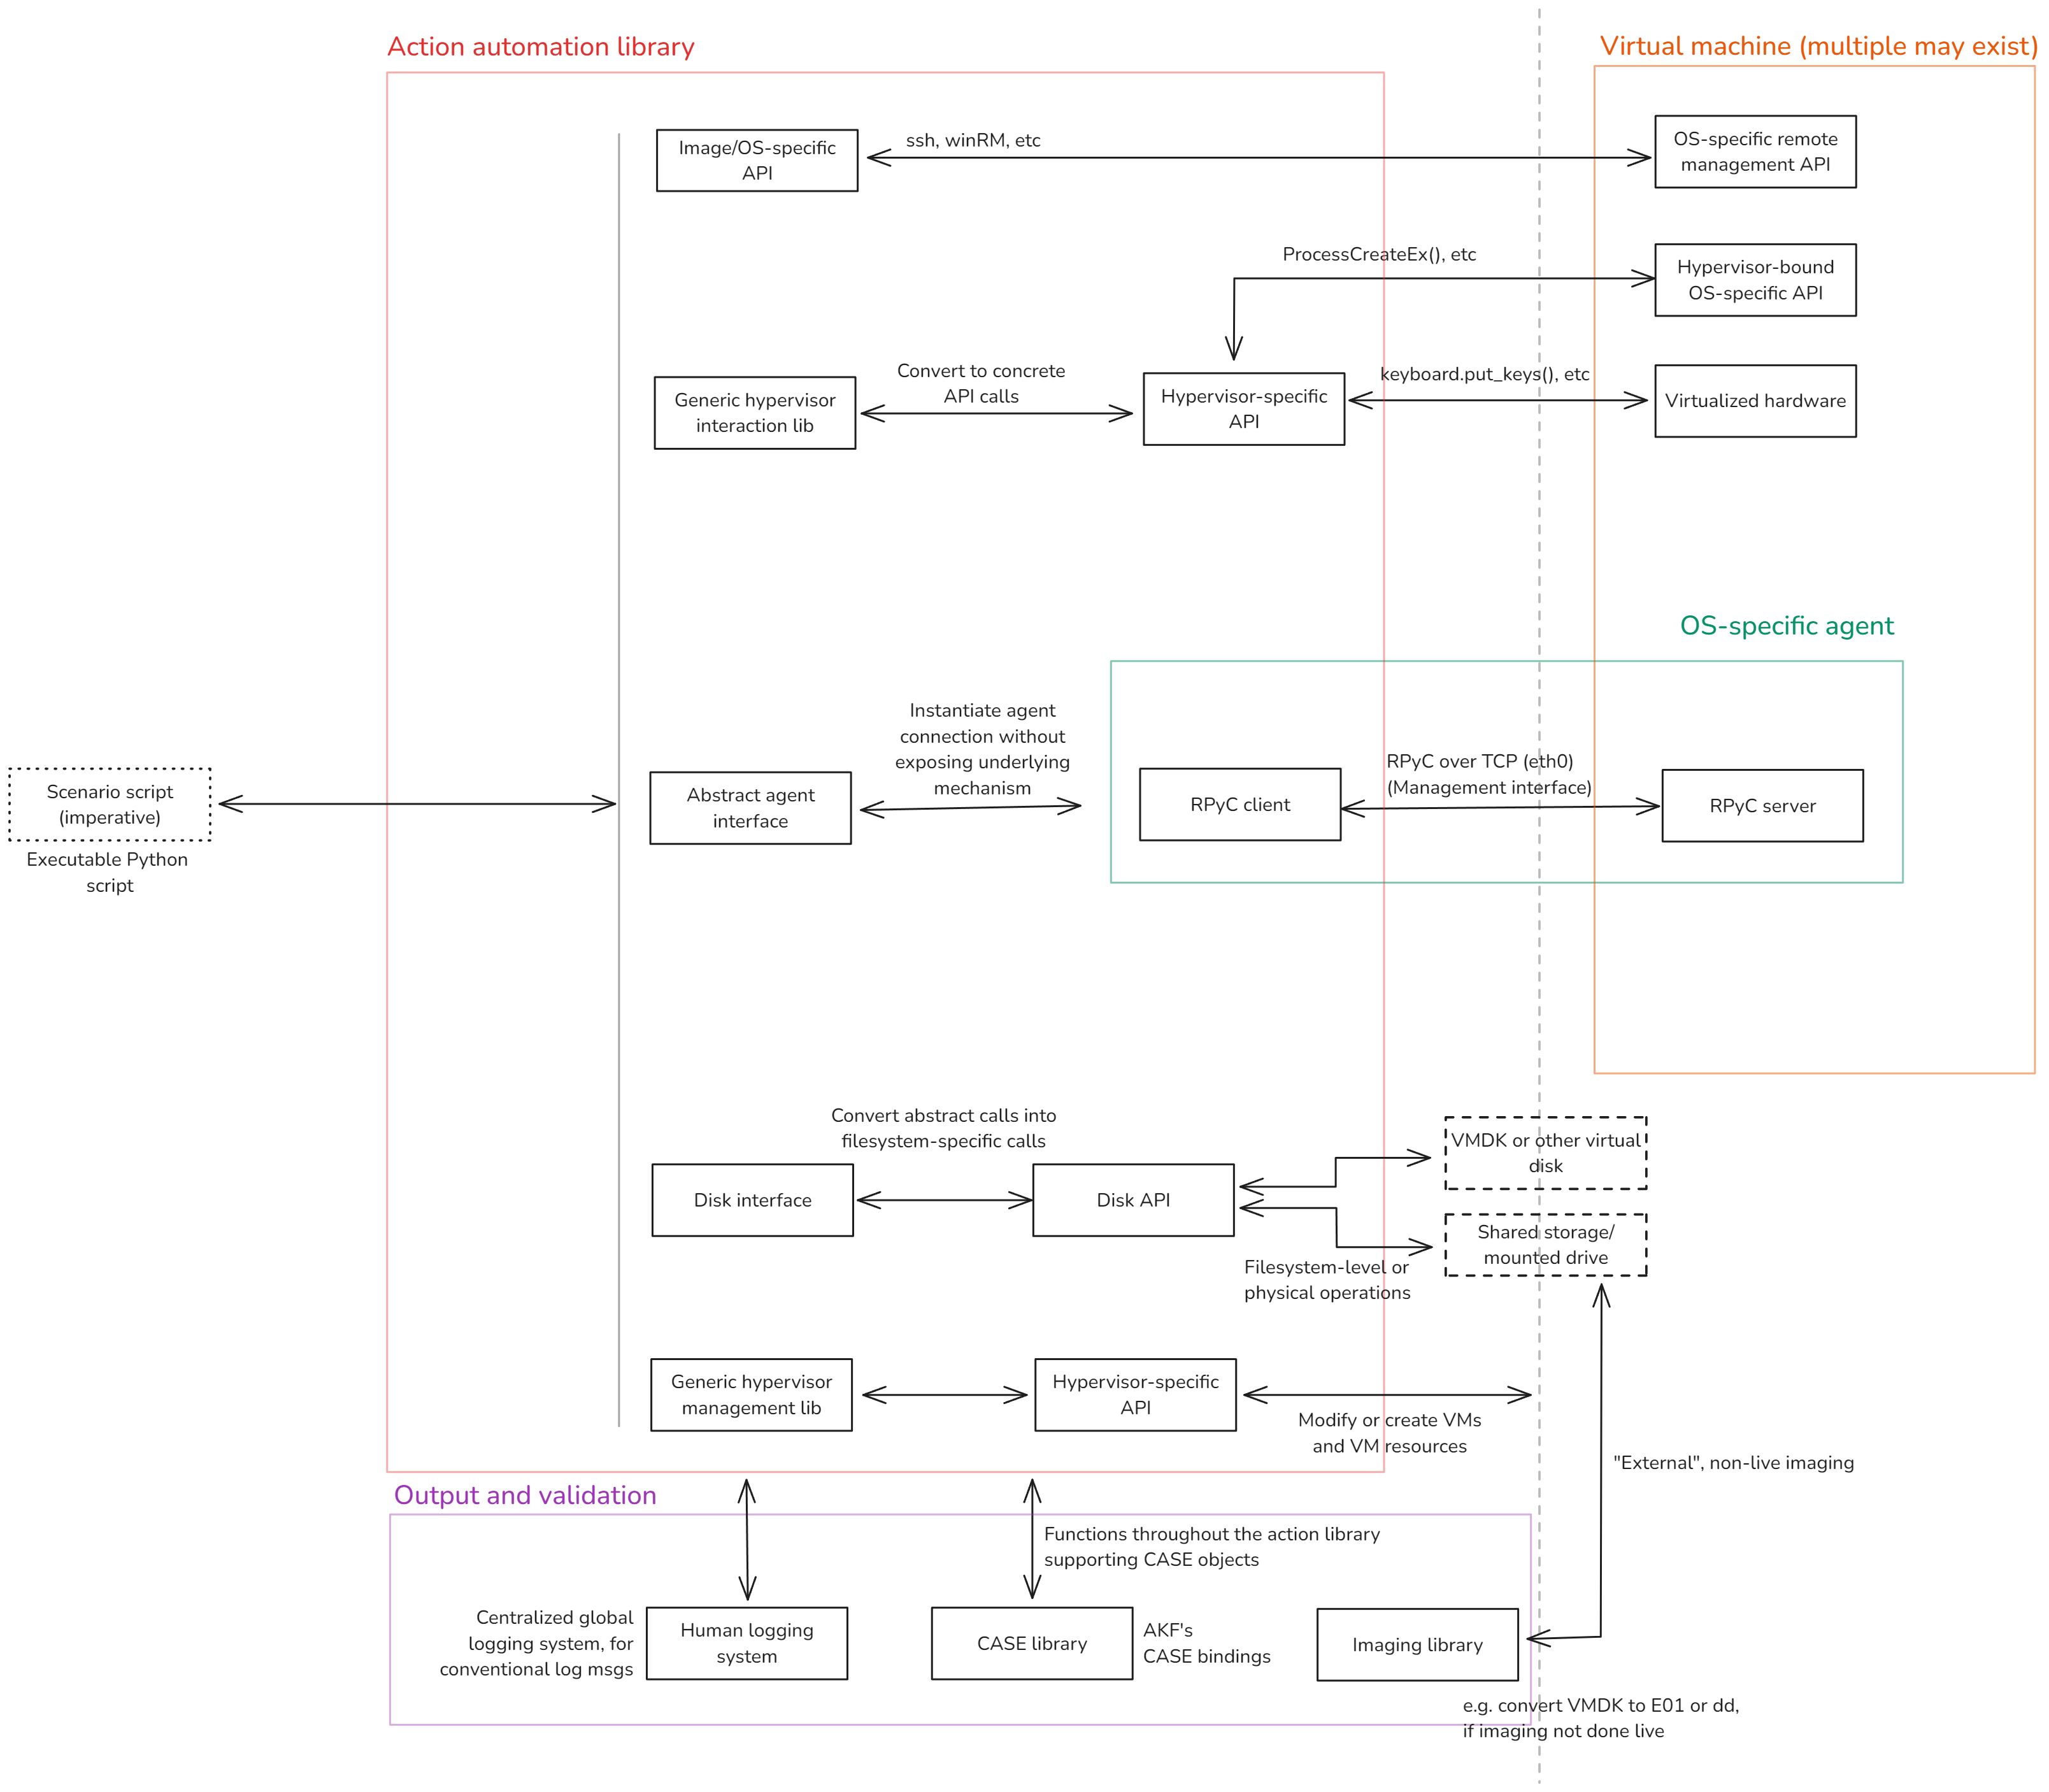
\includegraphics[width=1\linewidth]{architecture-full-b.png}
\caption{Detailed diagram of \passthrough{\lstinline!akflib!} and
related modules}\label{fig:architecture-full-b}
\end{figure}

The virtualized environment and its agent, also described throughout
\autoref{chapter-four}, is depicted in
\autoref{fig:architecture-full-d}. Note that some elements depicted in
this figure are described in \autoref{chapter-five} and
\autoref{chapter-six}.

\begin{figure}[h]
\centering
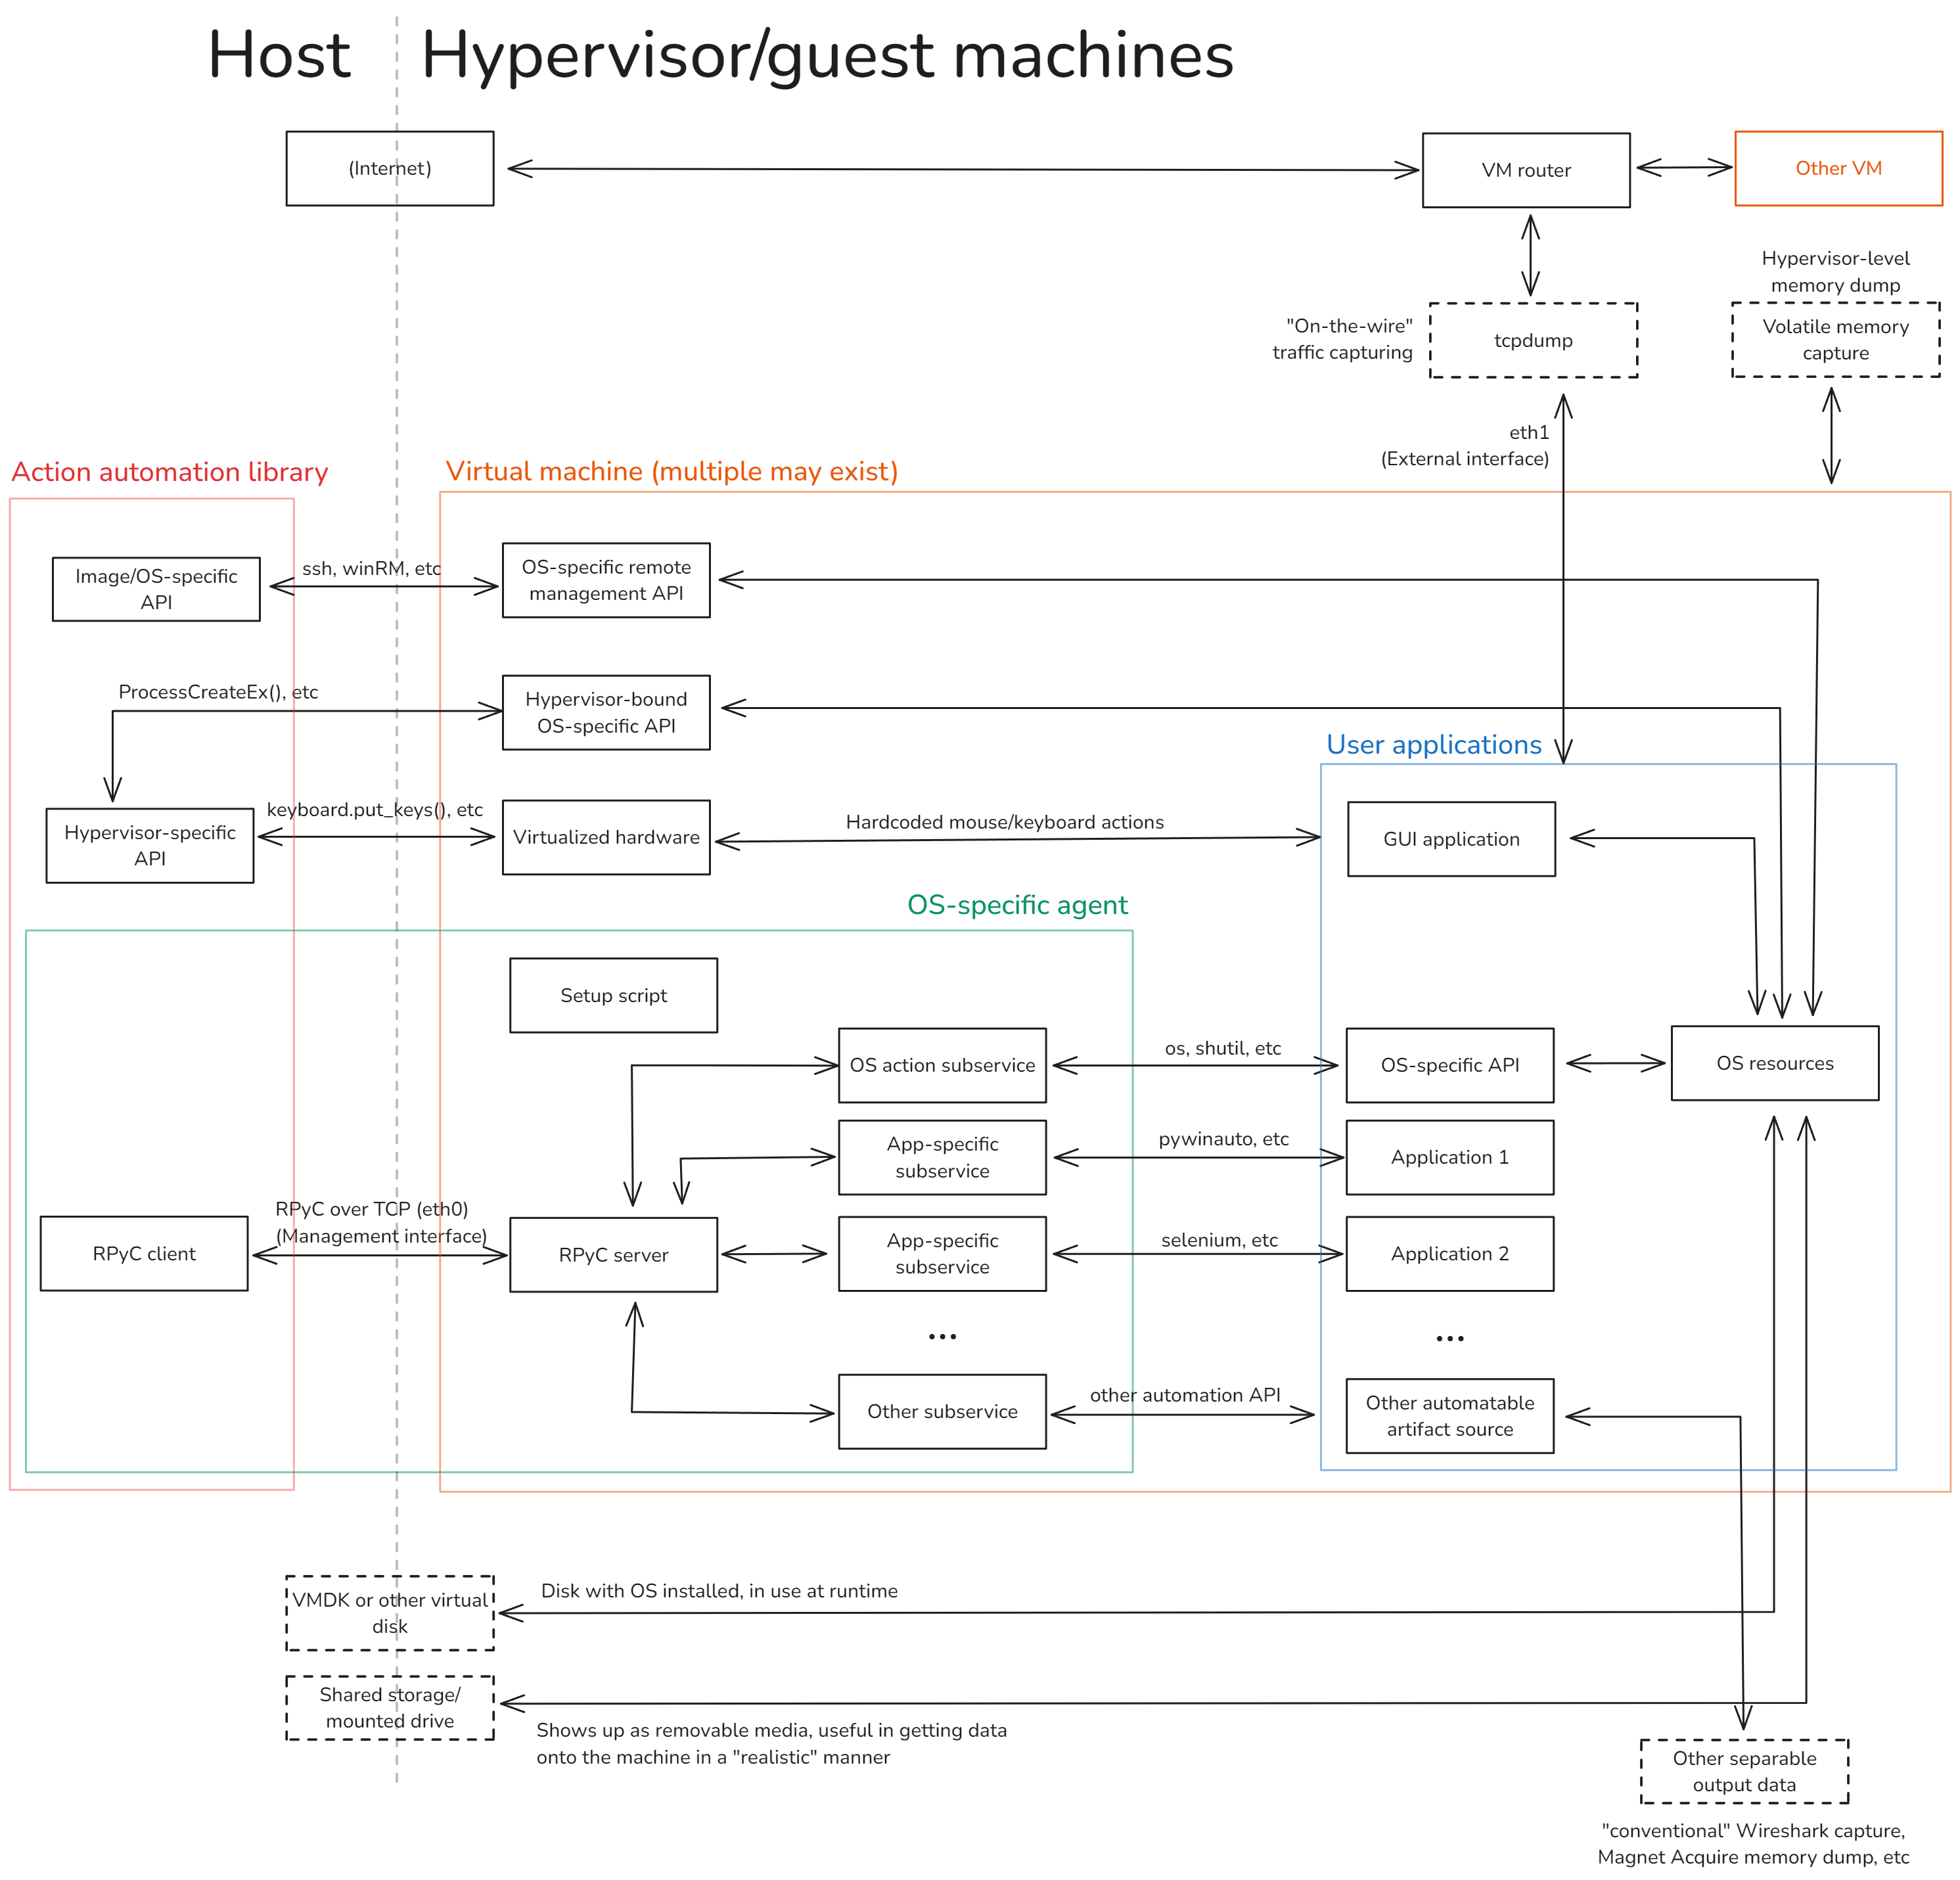
\includegraphics[width=1\linewidth]{architecture-full-d.png}
\caption{Detailed diagram of AKF's virtualized
environment}\label{fig:architecture-full-d}
\end{figure}

The output and validation library, described throughout \autoref{chapter-five}, is depicted in
\autoref{fig:architecture-full-c}. Note that this is distinct from
\autoref{fig:output-full}, which includes various virtual machine
outputs due to their role in the chapter's discussion.

\begin{figure}[h]
\centering
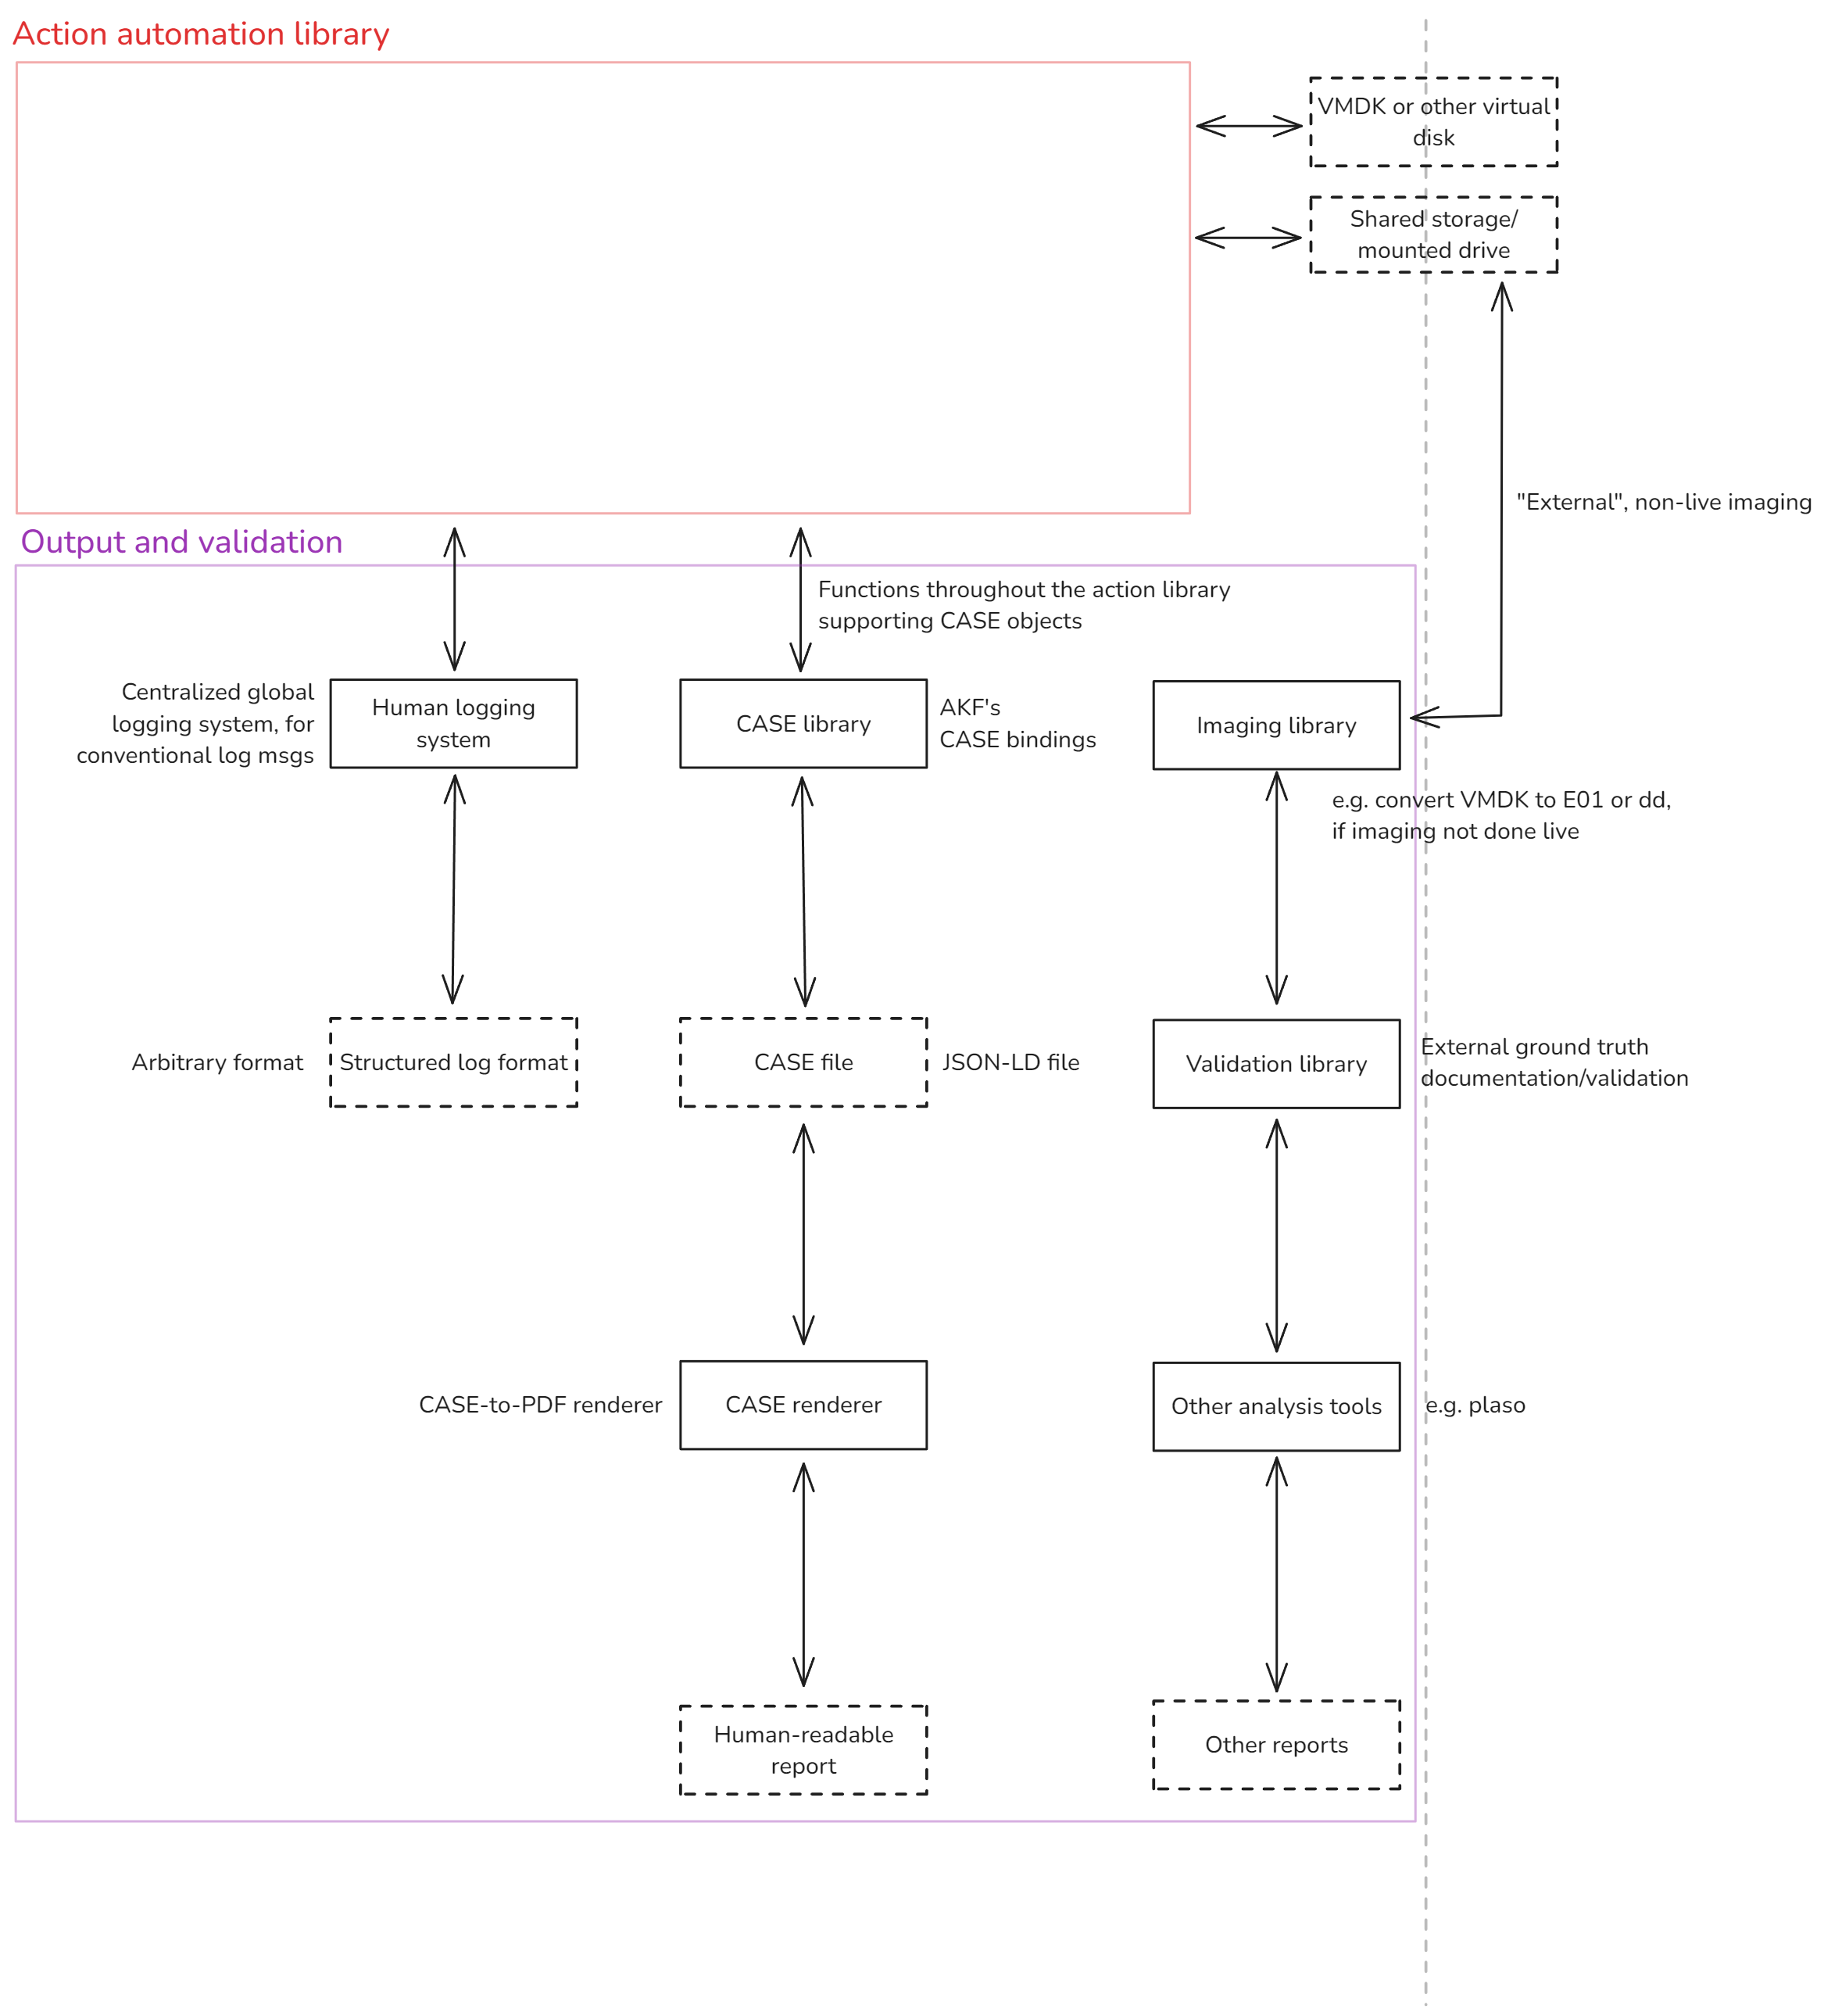
\includegraphics[width=1\linewidth]{architecture-full-c.png}
\caption{Detailed diagram of AKF modules responsible for output and
validation}\label{fig:architecture-full-c}
\end{figure}

Finally, modules related to scenario construction, as described in
\autoref{chapter-six}, are depicted in
\autoref{fig:architecture-full-a}.

\begin{figure}[h]
\centering
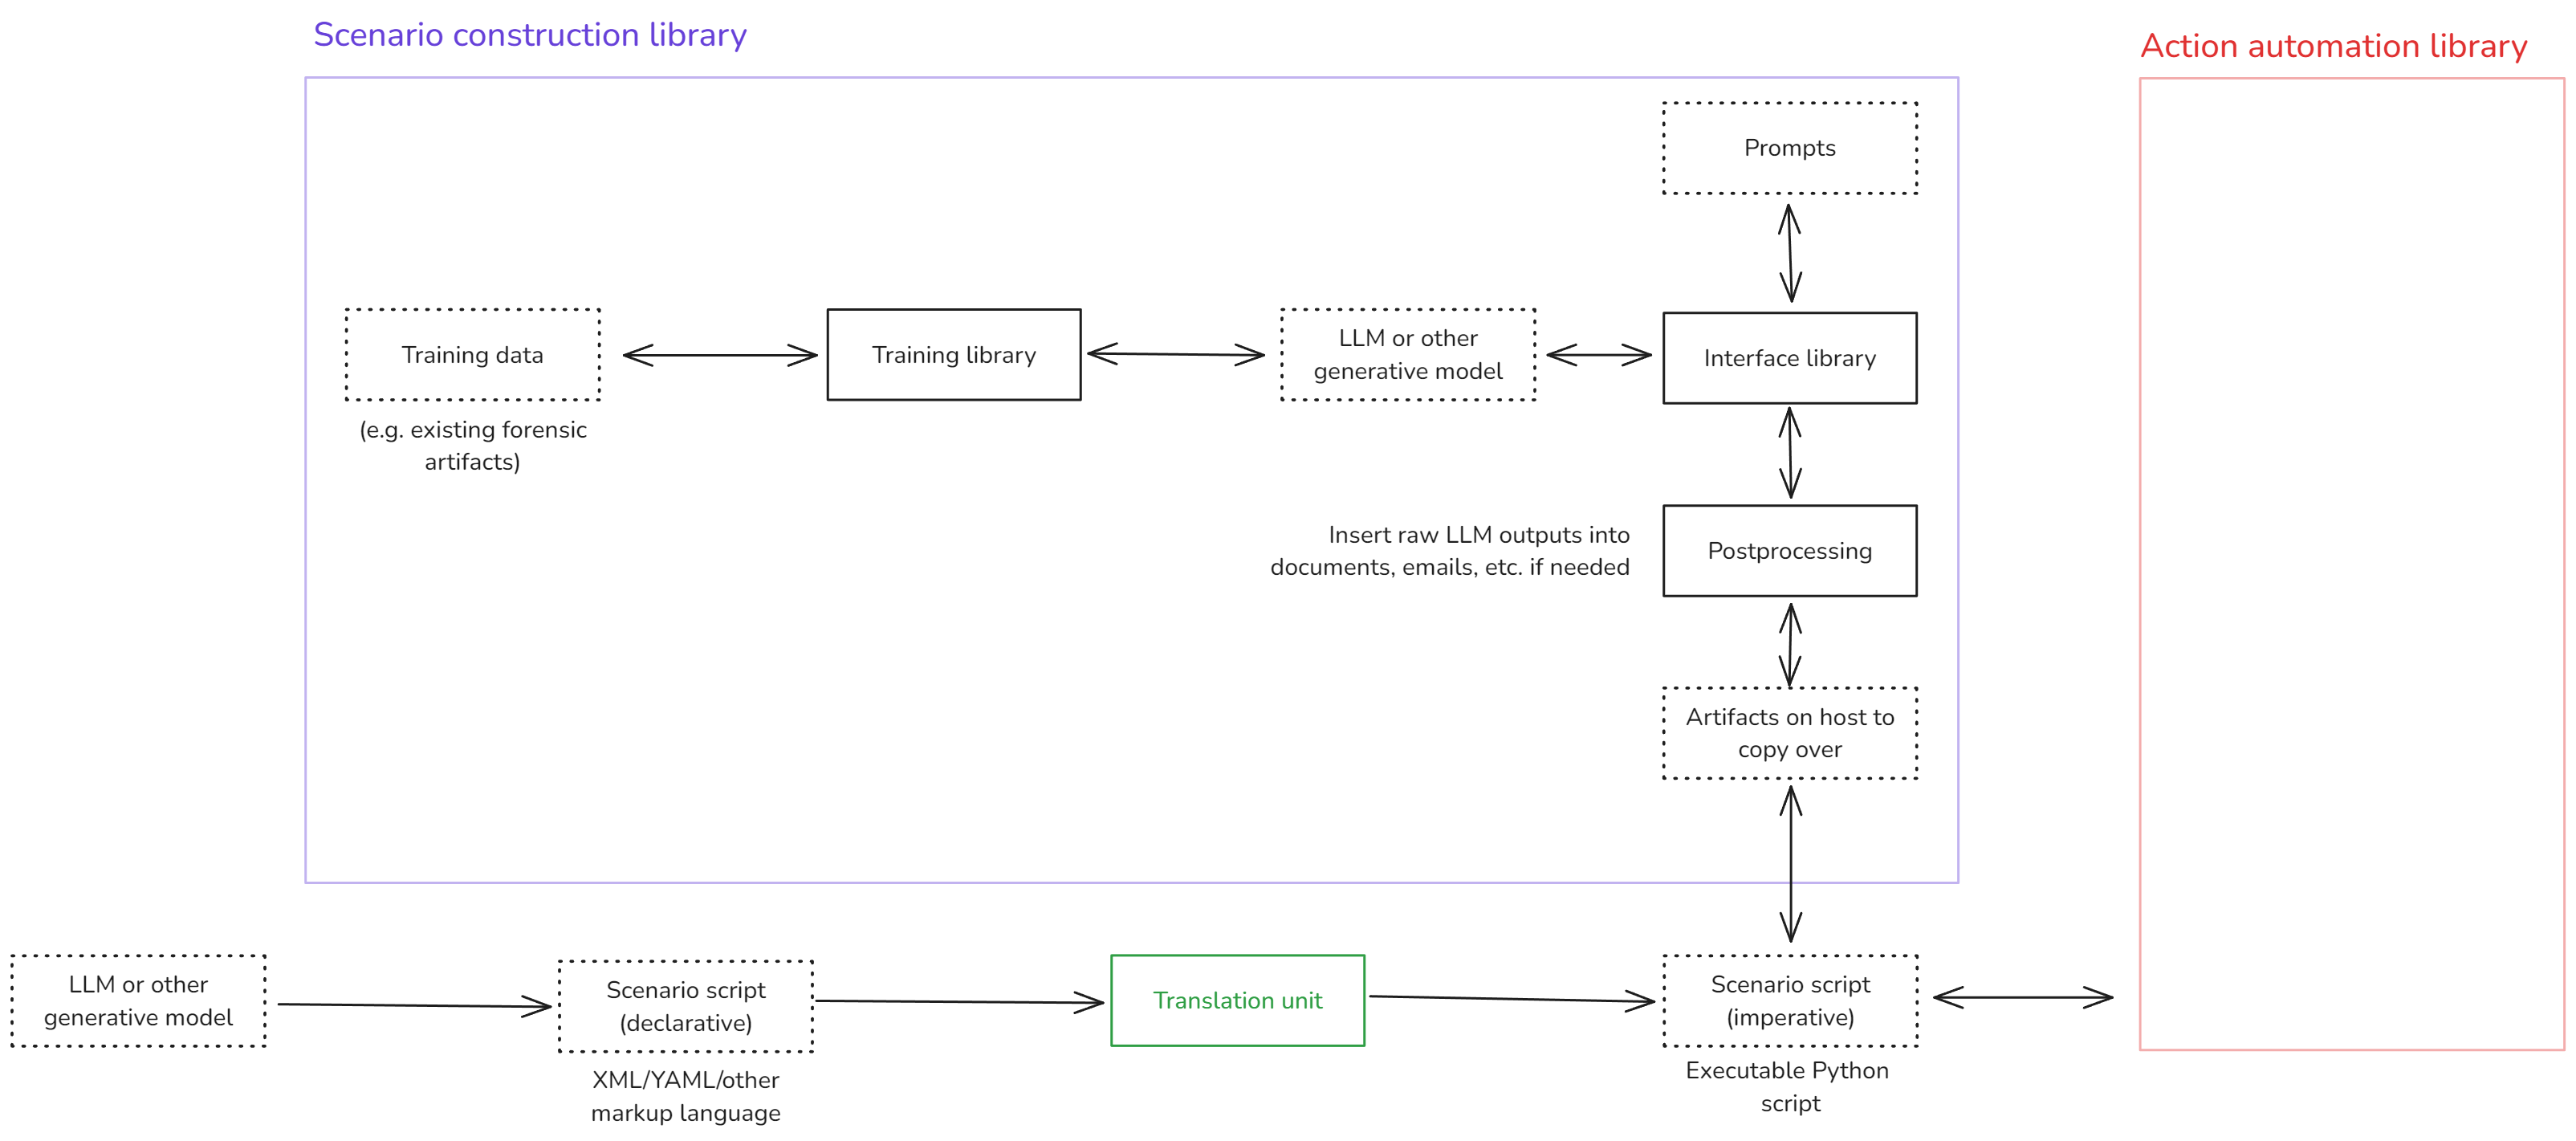
\includegraphics[width=1\linewidth]{architecture-full-a.png}
\caption{Detailed diagram of AKF modules related to scenario
construction}\label{fig:architecture-full-a}
\end{figure}

\chapter{Code samples}\label{appendix-b}

\section{Code repositories}\label{code-repositories}

The complete implementation of AKF is available on GitHub at the
following locations:

\begin{itemize}
\tightlist
\item
  Core libraries (\passthrough{\lstinline!akflib!}):
  \url{https://github.com/lgactna/akflib}
\item
  The AKF agent for Windows (\passthrough{\lstinline!akf\_windows!}):
  \url{https://github.com/lgactna/akf-windows}
\item
  Standalone CASE/UCO 2.0 bindings for Python
  (\passthrough{\lstinline!caselib!}):
  \url{https://github.com/lgactna/CASE-pydantic}
\end{itemize}

The \passthrough{\lstinline!akf\_windows!} repository contains a sample
declarative script utilizing every implemented declarative module,
demonstrating nearly all existing AKF functionality. It also contains an
equivalent imperative script that was generated using
\passthrough{\lstinline!akf-translate!}. Both scripts, and some of their
outputs, can be found in the \passthrough{\lstinline!./scenarios!}
folder.

\section{Comparison of ForTrace and AKF
agents}\label{comparison-of-fortrace-and-akf-agents}

Invoking commands in ForTrace
\cite{gobelForTraceHolisticForensic2022} is straightforward; at the
network level, commands are performed by issuing a simple string to the
agent running on the target VM. For example, invoking a command to add a
new user to the VM can be seen in \autoref{lst:b.2.a}:

\begin{lstlisting}[label={lst:b.2.a}, caption={Creating a new user through ForTrace agent commands}, language=Python]
# From Demo.py
guest = virtual_machine_monitor1.create_guest(guest_name=imagename, platform="windows")

# Wait for the VM to connect to the VMM
guest.waitTillAgentIsConnected()
# create userManagement object
userManagement_obj = guest.application("userManagement", {})

# Add different users
logger.info("Adding user1")
try:
    userManagement_obj.addUser("user1", "password")
    while userManagement_obj.is_busy is True:
        time.sleep(1)
except Exception as e:
    print("An error occured: ")
    print(e)
time.sleep(5)
\end{lstlisting}

The agent's main loop, which receives and interprets these commands, is
also straightforward. A simplified version of the main loop is depicted
in \autoref{lst:b.2.b}:

\begin{lstlisting}[label={lst:b.2.b}, caption={Simplified ForTrace agent entry point}, language=Python]
def main():
    # create logger
    logger = create_logger('guestAgent', logging.INFO)

    logger.info("create Agent")
    a = Agent(operating_system=platform.system().lower(), logger=logger)
    logger.info("connect to fortrace controller: %s:%i" % (fortrace_CONTROLLER_IP, fortrace_CONTROLLER_PORT))
    a.connect(fortrace_CONTROLLER_IP, fortrace_CONTROLLER_PORT)

    # let all network interfaces come up
    time.sleep(15)

    # inform fortrace controller about network configuration
    a.register()

    # wait for commands
    while 1:
        time.sleep(1)
        a.receiveCommands()
\end{lstlisting}

When the \passthrough{\lstinline!Agent!} is instantiated, it binds a TCP
socket to the configured port and IP address, where it expects the
server (the VMM) to issue commands.
\passthrough{\lstinline!Agent.receiveCommands()!} executes commands by
reading the socket, parsing the received content, and then invoking
\passthrough{\lstinline!Agent.do\_command()!}, which converts the
command message into a specific Python function call with arguments.

The server, or ``virtual machine monitor'' (VMM), issues commands over
TCP to a running instance of the agent on the VM. Each module under
\passthrough{\lstinline!fortrace.application!} can be thought of as a
coherent group of commands associated with a particular user application
(such as Firefox or Thunderbird). Recall from \autoref{lst:b.2.a} how we
found our \passthrough{\lstinline!userManagement!} application and
invoked \passthrough{\lstinline!addUser!}; a simplified snippet is
depicted in \autoref{lst:b.2.c}:

\begin{lstlisting}[label={lst:b.2.c}, caption={Minimal ForTrace application API usage}, language=Python]
userManagement_obj = guest.application("userManagement", {})
userManagement_obj.addUser("user1", "password")
\end{lstlisting}

At a high level, the \passthrough{\lstinline!application()!} call
attempts to import
\passthrough{\lstinline!fortrace.application.\{application\_name\}!}.
Although not enforced by a higher-level interface, each of these modules
contains subclasses of the following four classes (defined in
\passthrough{\lstinline!fortrace.application.application!}) at minimum,
with additional helper classes for OS-specific functionality or other
modularity as needed:

\begin{itemize}
\tightlist
\item
  \passthrough{\lstinline!ApplicationVmmSide!}: Contains one function
  for each command implemented in
  \passthrough{\lstinline!ApplicationGuestSide!}. Each function builds a
  message that will be interpreted and acted upon by the corresponding
  \passthrough{\lstinline!ApplicationGuestSideCommands!} class.
\item
  \passthrough{\lstinline!ApplicationVmmSideCommands!}: Accepts and
  interprets module-specific messages returned by the agent, which may
  be used to update the remote state as tracked by the host.
\item
  \passthrough{\lstinline!ApplicationGuestSide!}: Implements the actual
  application-specific functionality for the agent, providing one
  function for each available command.
\item
  \passthrough{\lstinline!ApplicationGuestSideCommands!}: Interprets
  commands and arguments, calling the respective function in the
  corresponding \passthrough{\lstinline!ApplicationGuestSide!} subclass.
  This allows the actual dispatch of commands to be delegated to this
  class, which is free to choose how actions are performed (such as the
  use of threading and multiprocessing) as well as any module-wide state
  it may need to maintain.
\end{itemize}

This naming convention is intentional, as individual modules dictate the
name of the module in camelcase. For example,
\passthrough{\lstinline!fortrace.application.userManagement!} contains
\passthrough{\lstinline!UserManagementVmmSide!},
\passthrough{\lstinline!UserManagementVmmSideCommands!}, and so on.
Discovering and getting handles to these classes is performed through
string manipulation of the relevant application's module name, as shown
in \autoref{lst:b.2.d} (an abridged version of the
\passthrough{\lstinline!Agent.do\_command()!} method):

\begin{lstlisting}[label={lst:b.2.d}, caption={Demonstration of ForTrace agent module discovery and command execution}, language=Python]
def do_command(self, command):
    com = command.split(" ")
    package = com[0]
    module = com[1]

    # load class moduleGuestSide and moduleGuestSideCommands
    name = "fortrace." + package + "." + module
    self.logger.debug("module to load: " + name)
    mod = __import__(name, fromlist=[''])
    self.logger.debug("module '" + module + "' will be loaded via __import__")
    class_commands = getattr(mod, module[0].upper() + module[1:] + 'GuestSideCommands')
    
    class_commands.commands(self, app_obj, " ".join(com[1:]))
\end{lstlisting}

In the example above,
\passthrough{\lstinline!UserManagementGuestSide.addUser()!} contains the
code to execute on the guest when \passthrough{\lstinline!addUser()!} is
called, such as adding the registry keys needed for a user to be
created. On the other hand,
\passthrough{\lstinline!UserManagementVmmSide.addUser()!} contains the
code to send a message over TCP that the agent will understand,
eventually leading to the execution of the agent's version of
\passthrough{\lstinline!addUser()!}.

More precisely, the \passthrough{\lstinline!ApplicationVmmSide!}
subclass effectively serves as the API for calling the associated
functions in the \passthrough{\lstinline!ApplicationGuestSide!} class
running on the virtual machine. This subclass, along with the complete
agent-side code, is stored in a single file. For example, the API and
code for opening a Firefox browser window can be seen in
\autoref{lst:b.2.e}:

\begin{lstlisting}[label={lst:b.2.e}, caption={Sample ForTrace agent API implementation}, language=Python]
class WebBrowserFirefoxVmmSide(ApplicationVmmSide):
    def open(self, url):
        """Sends a command to open a webBrowserFirefox on the associated guest.

        @param url: Website to open.
        """
        try:
            self.logger.info("function: WebBrowserFirefoxVmmSide::open")
            self.url = url
            self.window_id = self.guest_obj.current_window_id
            self.guest_obj.send(
                "application " + "webBrowserFirefox " + str(self.window_id) + " open " + self.webBrowserFirefox + " " + self.url)

            self.guest_obj.current_window_id += 1
        except Exception as e:
            raise Exception("error WebBrowserFirefoxVmmSide::open: " + str(e))

# Example usage:
browser = WebBrowserFirefoxVmmSide()
browser.open("google.com")
\end{lstlisting}

Calling the \passthrough{\lstinline!open()!} command from the host sends
a structured message to the agent, generally of the form seen in
\autoref{lst:b.2.f}:

\begin{lstlisting}[label={lst:b.2.f}, caption={Sample ForTrace agent protocol message}, ]
application webBrowserFirefox <window id> open Firefox <url>
\end{lstlisting}

Upon receiving this message, the agent's main loop will search for the
\passthrough{\lstinline!webBrowserFirefox!} module and import its
corresponding \passthrough{\lstinline!ApplicationGuestSideCommands!}
subclass. After any state management, the subclass will then search for
a function called \passthrough{\lstinline!open!} in its corresponding
\passthrough{\lstinline!ApplicationGuestSide!} class, as implemented in
\autoref{lst:b.2.g}:

\begin{lstlisting}[label={lst:b.2.g}, caption={Corresponding ForTrace agent-side call }, language=Python]
class WebBrowserFirefoxGuestSide(ApplicationGuestSide):
    def open(self, args):
        # docstring omitted
        try:
            arguments = args.split(" ")
            web_browser = arguments[0]
            url = arguments[1]

            if len(arguments) > 2:
                self.timeout = arguments[2]
            else:
                self.timeout = 30

            self.logger.info(self.module_name + "GuestSide::open")
            self.last_driven_url = url
            self.logger.debug("URL to call: " + url)

            self.logger.info("open url: " + url)

            self.helper.run_firefox()  # start ff session

            retval = self.helper.navigate_to_url(url)  # browse to the specified url
            if not retval:
                self.logger.warning("could not open url")

            self.agent_object.send("application " + self.module_name + " " + str(self.window_id) + " opened")

            self.agent_object.send("application " + self.module_name + " " + str(self.window_id) + " ready")
            self.window_is_crushed = False
        except Exception as e:
            # Some logging/teardown...
            self.window_is_crushed = True
            self.agent_object.send("application " + self.module_name + " " + str(self.window_id) + " error")
\end{lstlisting}

As described in \autoref{the-akf-agent}, this is achieved in AKF using RPyC services, which are analogous
to the \passthrough{\lstinline!ApplicationGuestSideCommands!} and
\passthrough{\lstinline!ApplicationGuestSide!} classes of individual
ForTrace modules. In addition to providing the RPyC services themselves,
agents also implement an API to call these services using typed
functions.

For example, suppose we wanted to implement functionality similar to the
ForTrace code above, allowing users to navigate to a webpage. An
equivalent RPyC service and its corresponding API may be implemented as
seen in \autoref{lst:b.2.h}:

\begin{lstlisting}[label={lst:b.2.h}, caption={Minimal reimplementation of ForTrace module as an RPyC service}, language=Python]
# Server-side code
class ChromiumService(AKFService):
    def exposed_set_browser(
        self, browser_type: Literal["msedge", "chrome"], profile: str = "Default"
    ) -> BrowserContext:
        # Various setup code...
        self.browser = chromium.launch_persistent_context(
            headless=False,
            user_data_dir=profile_path,
            channel=browser_type,
            args=[f"--profile-directory={profile}"],
        )

        return self.browser

# Client-side API
class ChromiumServiceAPI(WindowsServiceAPI):
    def __init__(self, host: str, port: int) -> None:
        """
        Initialize the API with an RPyC connection to the service.
        """
        self.rpyc_conn = rpyc.connect(
            host,
            port,
            config={"sync_request_timeout": None},
        )

    def set_browser(
        self, browser_type: Literal["msedge", "chrome"], profile: str = "Default"
    ) -> BrowserContext:
        self.browser = self.rpyc_conn.root.set_browser(browser_type, profile)
        return self.browser
\end{lstlisting}

Implementing support for a particular service on the client-side API is
as simple as calling an untyped function
\passthrough{\lstinline!rpyc\_conn.root.set\_browser()!}. By wrapping it
around a typed function,
\passthrough{\lstinline!ChromiumServiceAPI.set\_browser()!}, users
regain the ability to use code completion and static linting tools.

\section{CASE Python bindings}\label{case-python-bindings}

As described in \autoref{case-and-python-bindings}, CASE is defined using Turtle, allowing objects to be
written in a human-readable text format. For example, the following set
of triples in \autoref{lst:b.3.a} describes an object called
\passthrough{\lstinline!ApplicationFacet!} with two properties,
\passthrough{\lstinline!numberOfLaunches!} and
\passthrough{\lstinline!applicationIdentifier!}:

\begin{lstlisting}[label={lst:b.3.a}, caption={Example CASE object definition for applications \cite{UcoProjectUCO2025}}, ]
observable:ApplicationFacet
    a
        owl:Class ,
        sh:NodeShape
        ;
    rdfs:subClassOf core:Facet ;
    rdfs:label "ApplicationFacet"@en ;
    rdfs:comment "An application facet is a grouping of characteristics unique to a particular software program designed for end users."@en ;
    sh:property
        [
            sh:datatype xsd:integer ;
            sh:maxCount "1"^^xsd:integer ;
            sh:nodeKind sh:Literal ;
            sh:path observable:numberOfLaunches ;
        ] ,
        [
            sh:datatype xsd:string ;
            sh:maxCount "1"^^xsd:integer ;
            sh:nodeKind sh:Literal ;
            sh:path observable:applicationIdentifier ;
        ] ,
        ...
        ;
    sh:targetClass observable:ApplicationFacet ;
    .
\end{lstlisting}

An instance of an \passthrough{\lstinline!Application!} object may thus
be represented in the JSON-LD format using the
\passthrough{\lstinline!ApplicationFacet!} as seen in
\autoref{lst:b.3.b}, including some attributes omitted from the example
in \autoref{lst:b.3.a}:

\begin{lstlisting}[label={lst:b.3.b}, caption={Instantiated CASE application object as JSON-LD }, ]
{
    "@id": "kb:dcec8d09-a8bc-4b7c-93ab-16c7b363d48b",
    "@type": "uco-observable:Application",
    "uco-core:hasFacet": [
        {
            "@id": "kb:68004de9-1139-405f-aea7-2c05f3a84709",
            "@type": "uco-observable:ApplicationFacet",
            "uco-observable:numberOfLaunches": 12,
            "uco-observable:applicationIdentifier": "test"
        },
    ]
}
\end{lstlisting}

The CASE project provides official Python bindings
\cite{CaseworkCASEMappingPython}. One notable implementation detail
is that it stores all object attributes in a dictionary after
instantiation. This can be seen in the example of an
\passthrough{\lstinline!ApplicationFacet!} in \autoref{lst:b.3.c} below.
Intuitive usage suggests that the
\passthrough{\lstinline!application\_identifier!} attribute is
accessible through the \passthrough{\lstinline!facet!} object, but it
must instead be accessed as a dictionary key with a non-intuitive name.

\begin{lstlisting}[label={lst:b.3.c}, caption={Sample usage of official CASE Python bindings \cite{CaseworkCASEMappingPython}}, language=Python]
facet = ApplicationFacet(application_identifier = "test", number_of_launches=3)

# These attributes do not exist
facet.application_identifier
facet.number_of_launches

# The number of launches must be accessed as a dictionary key, which
# does not return a simple integer; instead, it returns a
# dictionary
app_facet['uco-observable:numberOfLaunches']
# -> {"@type": "xsd:integer", "@value": "3"}
\end{lstlisting}

AKF's Pydantic-based bindings greatly simplify the declaration of
individual CASE objects while allowing typical attribute-based access.
For example, AKF's complete declaration of
\passthrough{\lstinline!ApplicationFacet!} is shown in
\autoref{lst:b.3.d}:

\begin{lstlisting}[label={lst:b.3.d}, caption={Example of Pydantic-based CASE object declaration used by AKF}, language=Python]
from typing import Optional

from uco import core

# ... Other object definitions in same file

class ApplicationFacet(core.Facet):
    installedVersionHistory: ApplicationVersion | list[ApplicationVersion] | None = []
    operatingSystem: ObservableObject | None = Field(
        default=None, json_schema_extra={"IRI": True}
    )
    numberOfLaunches: int | None = None
    applicationIdentifier: str | None = None
    version: str | None = None
\end{lstlisting}

This definition is only eight lines, which is 27 lines shorter than the
declaration of \passthrough{\lstinline!ApplicationFacet!} provided by
the CASE project's existing Python bindings (excluding the docstring).

A simple CASE bundle, representing the complete contents of a forensic
scenario, can be constructed and exported to JSON-LD using AKF libraries
as shown in \autoref{lst:b.3.e}:

\begin{lstlisting}[label={lst:b.3.e}, caption={Demonstration of bundle serialization using the AKF Python bindings for CASE}, language=Python]
from caselib import case, uco

bundle = uco.core.Bundle(
    description="An Example Case File",
    specVersion="UCO/CASE 2.0",
    tag="Sample artifacts",
)

url_object = uco.observable.ObservableObject()
url_facet = uco.observable.URLFacet(fullValue="www.docker.com/howto")
url_object.hasFacet.append(url_facet)
bundle.object.append(url_object)

with open("example.jsonld", "wt+") as f:
    data = bundle.model_dump(serialize_as_any=True)
    f.write(json.dumps(data, indent=2))
\end{lstlisting}

Although the UCO/CASE 2.0 Python bindings developed as part of AKF
significantly improve usability and flexibility over the existing CASE
bindings, several limitations of the library do not make it fully
compliant with the CASE ontology. In particular, the Python bindings aim
to keep object definitions as simple as possible, preferring native
Python types where possible. This means that some information from the
ontology is lost when converting them to their respective Python class.
Several examples include:

\begin{itemize}
\tightlist
\item
  \textbf{Datatypes}: Many XSD datatypes are not equivalent between the
  turtle files and Python bindings. For example, the arbitrary-precision
  \passthrough{\lstinline!xsd:decimal!} type is represented as a native
  Python float, but is also written out as a native JSON float on
  serialization to JSON-LD. The resulting datatype is
  \passthrough{\lstinline!xsd:float!}, which may cause information to be
  lost.
\item
  \textbf{Vocabularies}: Many CASE ``vocabularies'', a datatype in which
  a field's value should be chosen from a fixed set of values, are
  correctly converted to native Python string enumerations. However, the
  vocabulary datatype is not serialized, only the value; thus, the
  resulting JSON-LD makes no indication that the selected value is
  actually from the vocabulary datatype, even if the value itself is
  inside the vocabulary set. For example, if the string ``MD5'' is a
  member of the \passthrough{\lstinline!HashNameVocab!} datatype, our
  Python bindings serialize this as a standard
  \passthrough{\lstinline!xsd:string!}, not
  \passthrough{\lstinline!vocabulary:HashNameVocab!}.
\item
  \textbf{Field names}: Some fields of CASE objects, such as the
  \passthrough{\lstinline!from!} field of an email message, are reserved
  Python keywords that may not be used as the name of a variable. To
  solve this, we append an underscore to any fields that would violate
  this rule when automatically generating Pydantic classes from the
  Turtle RDF files. However, the original name of the field is not
  preserved when serializing objects; although the simplest fix is to
  remove trailing underscores when serializing, a more robust solution
  may be to attach the ``original'' name to the Pydantic field.
\item
  \textbf{Dangling references}: There are no built-in mechanisms to
  ensure that an object is serialized in its ``full'' form at least
  once; that is, a user could place references to an object identifier
  throughout the document without adding the object being referred to.
\end{itemize}

Additionally, one major feature of CASE/UCO is not currently supported.
CASE allows objects to be of multiple types at once, such as a disk
image marked as both an \passthrough{\lstinline!observable:File!} and an
\passthrough{\lstinline!observable:Image!}. Python types can inherit
from multiple types, but a single object may not be multiple types at
once; it might be necessary to create a ``wrapper'' type that
encompasses both types and correctly serializes these types as expected.

\section{Historical declarative
syntaxes}\label{historical-declarative-syntaxes}

While designing the declarative syntax for AKF, the syntaxes of D-FET
\cite{williamCloudbasedDigitalForensics2011}, SFX
\cite{russellForensicImageDescription2012}, and Yannikos et al.
\cite{yannikosDataCorporaDigital2014} were reviewed. For
completeness, brief examples of scenarios in each of these synthesizers
are included here. Notably, none of these works provide details on how
the parser of their declarative languages is implemented. Similarly, few
details are provided about the architecture and design of the code used
to carry out actions based on interpreted declarative instructions. This
lack of detail may be attributed to the fact that the scenario creation
enabled by these declarative syntaxes, rather than the syntaxes
themselves, was the primary focus of these works.

\textbf{D-FET} \cite{williamCloudbasedDigitalForensics2011} uses a
custom language that does not depend on any existing text-based
languages, as seen in the simple scenario in \autoref{lst:b.4.a}:

\begin{lstlisting}[label={lst:b.4.a}, caption={Sample D-FET declarative scenario without events \cite{williamCloudbasedDigitalForensics2011}}, ]
INSTANCE LOAD [Image=WINDOWS2003] 
MOUNT INSTANCE [Disk=STANDARDDISK] AS [Partition="c"] 
ACTIVITY LOAD [Number=12] [Type=JPEG IMAGES; Class=DRUGS] 
    INTO [Folder=USER FOLDER] 
    AT [Period=1 MINUTE] [Interval=INTERVAL] 
    FOR [User=Fred]
\end{lstlisting}

The scenario above will create an instance based on the WINDOWS2003
image from the Host Forensics Image library (which contains pre-created
images from OS installation discs). It will then load 12 JPEG images
from the ``DRUGS'' class of images using the ``STANDARDDISK'' disk
image. This appears to create a host with \emph{predefined}, but not
\emph{timed} activity -- the machine simply begins in this state rather
than simulating a user doing this over some period of time.

To generate timed activity that can be placed on a timeline, D-FET
allows users to add ``events.'' The sequence of events in
\autoref{lst:b.4.b} directs the synthesizer to log in as a user, delete
files, and log out.

\begin{lstlisting}[label={lst:b.4.b}, caption={Extension of the D-FET declarative scenario with events \cite{williamCloudbasedDigitalForensics2011}}, ]
INSTANCE LOAD [Image=WINDOWS2003] 
MOUNT INSTANCE [Disk=STANDARDDISK] AS [Partition="c"] 
ACTIVITY LOAD [Number=12] [Type=JPEG IMAGES; Class=DRUGS] 
    INTO [Folder=USER FOLDER] 
    AT [Period=1 MINUTE] [Interval=INTERVAL] 
    FOR [User=Fred]
ACTIVITY EVENT [Event=LOGIN; User=Fred] 
ACTIVITY EVENT [Event=DELETEFILE; User=Fred; File=JPEF IMAGES] 
ACTIVITY EVENT [Event=LOGOUT; User=Fred ]
\end{lstlisting}

\textbf{SFX} \cite{russellForensicImageDescription2012} uses an
XML-based language with tags and attributes that are easily readable ,
as shown in \autoref{lst:b.4.c}:

\begin{lstlisting}[label={lst:b.4.c}, caption={Sample SFX declarative scenario expressed as XML \cite{russellForensicImageDescription2012}}, language=XML]
<disk size="512M" alignment="cylinder" diskid="0x12345678">
    <partition index="p1" hidden="0" size="48M" type="vfat">
        <expand archive="part1.zip" />
        <copy from="fake.dat" to="/fake01.dat" />
        <copy from="fake.dat" to="/fake02.dat" />
        <delete from="/Thomas.jpg" />
    </partition>
    <partition index="p2" hidden="0" size="48M" type="ntfs">
        <base os="windows7x64" />
        <copy from="fake.dat" to="/fake03.dat" />
        <copy from="fake.dat" to="/fake04.dat" />
        <user username="Gordon">
            <browserhistory browser="firefox">
                <url link="[http://bbc.co.uk"](http://bbc.co.uk") time="13:14:00 1 Jan 2013" />
            </browserhistory>
        </user>
    </partition>
    <partition index="p3" hidden="1" size="64M" type="ntfs">
        <expand archive="part3.zip" />
        <copy from="fake.dat" to="/fake11.dat" />
        <copy from="fake.dat" to="/fake12.dat" />
        <delete from="/docs/image.exe" />
        <slackspace offset="20" file="/tomas.gif" message="This is a secret message" />
    </partition>
    <partition index="s1" hidden="0" size="144M" type="ext3">
        <base os="fedora15x64" />
        <expand archive="part2.tar" />
        <copy from="fake.dat" to="/tmp/fake01.dat" />
        <copy from="fake.dat" to="/tmp/fake02.dat" />
    </partition>
</disk>
\end{lstlisting}

Here, a user can define multiple partitions on a single disk, each with
a distinct filesystem that may or may not contain an underlying
operating system. SFX allows users to generate artifacts in multiple
ways, with each unique application- or OS-specific feature using a
distinct XML element name. Artifact generation features include copying
files to the guest machine in bulk, inserting files in the slack space
of an existing file, and using browser artifacts.

Finally, the work of Yannikos et al.
\cite{yannikosDataCorporaDigital2014} is particularly notable
because it appears to be fully GUI-based, expecting users to visually
construct Markov chains to define scenarios. An example scenario from
their publication can be seen in Figure \autoref{fig:yannikos-gui}:

\begin{figure}[h]
\centering
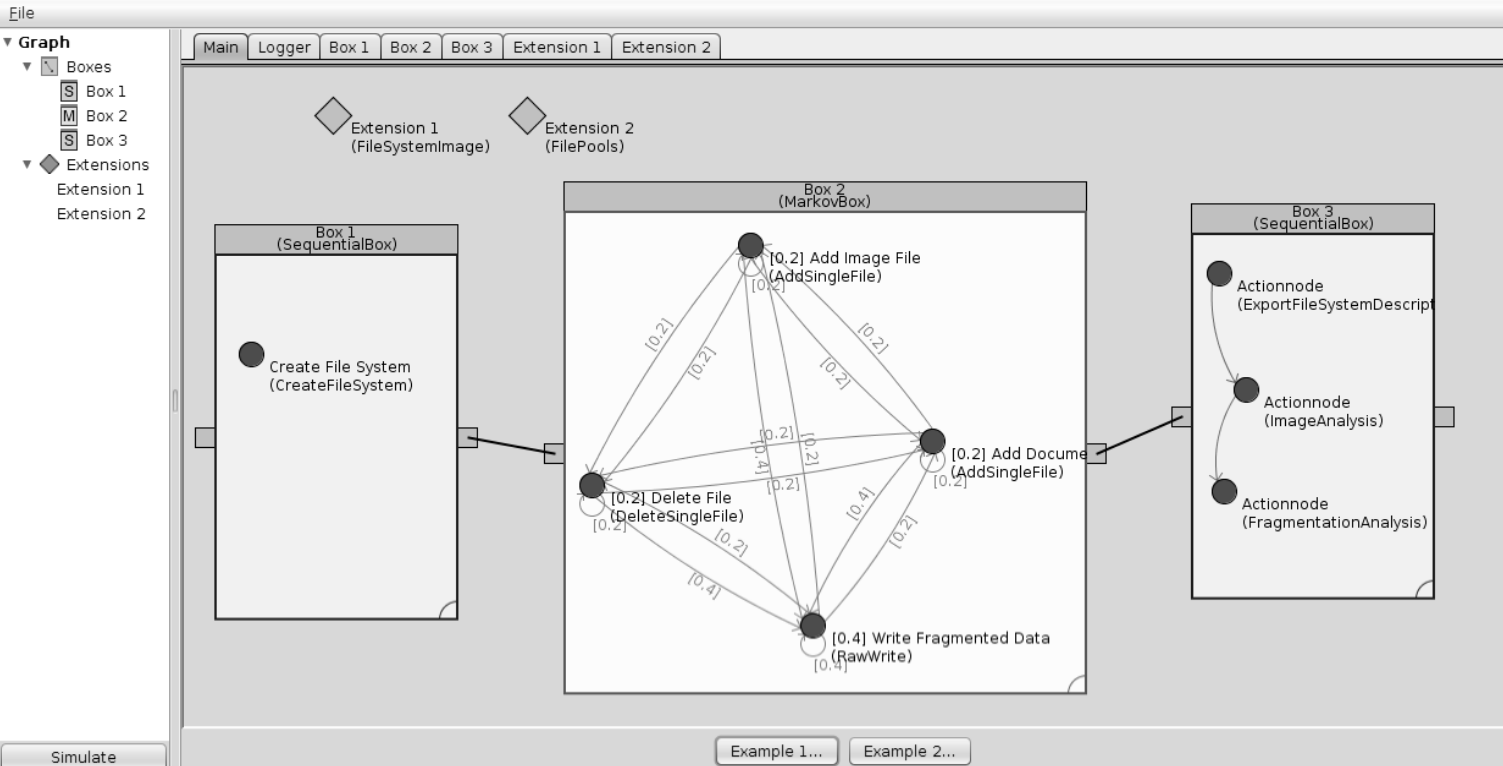
\includegraphics[width=1\linewidth]{yannikos.png}
\caption{GUI-based scenario declaration from Yannikos et al.
\cite{yannikosDataCorporaDigital2014}}\label{fig:yannikos-gui}
\end{figure}

Although details are relatively limited, each node appears to be a
distinct action that can be automated. Individual nodes accept
parameters that can be used to configure how their associated artifacts
are created. Each ``box'' encompasses a complete Markov chain, with
transitions from one box to another occurring after an unknown condition
is fulfilled. Finally, the diamonds outside the boxes, known as
extensions, are libraries that provide extra functionality during the
execution of the overall scenario.



\end{document}